\documentclass[11pt, a4paper]{report}
\usepackage{polski}
\usepackage[cp1250]{inputenc}
\usepackage{color}
\usepackage[table]{xcolor}
\usepackage{listings}
\usepackage{caption}
\usepackage{enumitem}
\usepackage{graphics}
\usepackage{epsfig}
\usepackage{rotating}
\usepackage{fancyhdr}
\usepackage{subfig}
\usepackage{url}
\usepackage{float}

\usepackage{booktabs}
\newcommand{\ra}[1]{\renewcommand{\arraystretch}{#1}}

\renewcommand{\abstractname}{Abstract}

\restylefloat{figure} 

\renewcommand{\figurename}{Rys.}
\renewcommand{\tablename}{Tab.}
\renewcommand{\lstlistlistingname}{Spis listing�w}


%% Define a new 'leo' style for the package that will use a smaller font.
\makeatletter
\def\url@leostyle{%
  \@ifundefined{selectfont}{\def\UrlFont{\sf}}{\def\UrlFont{\small\ttfamily}}}
\makeatother
%% Now actually use the newly defined style.
\urlstyle{leo}

\pagestyle{fancy}


\pagestyle{fancy}
\rhead{}
\lhead{\nouppercase{\leftmark}}



\lstdefinelanguage{apache}{
morekeywords={ServerAdmin, ServerName, ServerAlias, DocumentRoot, Options, AllowOverride, Order, ErrorLog, LogLevel, CustomLog, allow},
sensitive=false,
morestring=[b]"
}

\definecolor{bbb}{gray}{0.90}

\newcommand{\lstMikro}[1]
{\lstinline[breakatwhitespace=true, postbreak=\kern-3ex, basicstyle=\small\ttfamily,breaklines=true,language=bash,literate={\`}{}{0\discretionary{-}{}{}}]$#1$}

\lstset{
         basicstyle=\scriptsize\ttfamily, % Standardschrift
			numbers=left,
         numberstyle=\tiny,          % Stil der Zeilennummern
         %stepnumber=2,               % Abstand zwischen den Zeilennummern
         numbersep=5pt,              % Abstand der Nummern zum Text
         tabsize=2,                  % Groesse von Tabs
         extendedchars=true,         %
         breaklines=true,            % Zeilen werden Umgebrochen
         keywordstyle=\color{blue},
         stringstyle=\color{red}\ttfamily, % Farbe der String
         xleftmargin=17pt,
         framexleftmargin=17pt,
         framexrightmargin=6pt,
			framextopmargin=0pt,
         backgroundcolor=\color{bbb},
         showstringspaces=false     % Leerzeichen in Strings anzeigen ?        
 }

\floatstyle{ruled}
\newfloat{program}{thp}{lop}
\floatname{program}{Listing}

\DeclareCaptionFont{white}{\color{white}}
\DeclareCaptionFormat{listing}{\colorbox{gray}{\parbox{\textwidth}{#1#2#3}}}
\captionsetup[lstlisting]{format=listing,labelfont=white,textfont=white}

\makeatletter
\newcommand{\linia}{\rule{\linewidth}{0.4mm}}

% new itemize environment with itemsep parameter
\newenvironment{packed_item}[1][0]
  { \begin{itemize}
    % set spacing between items
    \addtolength{\itemsep}{#1\baselineskip}
    % set spacing between lines
    \addtolength{\baselineskip}{#1\baselineskip} }
  { \end{itemize} }


\renewcommand{\maketitle}{\begin{titlepage}

    \vspace*{1cm}

    \begin{center}\small
    Politechnika ��dzka\\
    Wydzia� Fizyki Technicznej i Matematyki Stosowanej\\
    Informatyka\\
    Systemy Informatyczne i Bazy Danych
    \end{center}

    \vspace{3cm}

    \noindent\linia

    \begin{center}

      \LARGE \textsc{\@title}

         \end{center}

     \linia

    \vspace{0.5cm}

    \begin{flushright}

    \textit{\small Autor:}\\

    \normalsize \textsc{\@author} \par

    \vspace{1cm}

     \textit{\small Opiekun:}\\

         dr in�. Anety Poniszewska - Mara�da
		
     \end{flushright}

    \vspace*{\stretch{6}}

    \begin{center}

    \@date

    \end{center}

  \end{titlepage}%

}

\makeatother

\title{Optymalizacja wydajno�ci aplikacji internetowych}
\author{�ukasz Adamczewski}
\begin{document}



\includepdf[pages={1}]{tytul.pdf}

    %podzi�kowania
    \newpage
    ~   %potrzebne dla \vfill
    \vfill
    {\sffamily
    \begin{flushright}
        \begin{tabular}{l}
        Chcia�bym w~tym miejscu podzi�kowa�:\\
        \\
        Narzeczonej Oliwii\\
        za wsparcie i wyrozumia�o�� podczas pisania pracy\\
        \\
        Rodzicom\\
        za pomoc w rozwijaniu pasji,\\dbaj�c o kondycje zdrowia psychicznego\\
			\\
        Pani promotor dr in�. Anecie Poniszewskiej - Mara�dzie\\
        za wnikliw� analiz� i pomoc podczas pisania pracy.\\
        \end{tabular}
    \end{flushright}
    }
    \vskip0.5in
    \thispagestyle{empty}
    \newpage
    %koniec podzi�kowa�

\tableofcontents


\chapter{Wst�p}

Niniejsza praca dyplomowa dotyczy zagadnie� in�ynierii oprogramowania oraz technologii baz danych wykorzystanych w dziedzinie \textit{e-commerce}. G��wny cel bada� stanowi przedstawienie realnych korzy�ci biznesowych wynikaj�cych z zastosowania szerokiego spektrum usprawnie� aplikacji internetowych. 

W tre�ci pracy przedstawiona jest analiza technik optymalizacji aplikacji internetowych z uwzgl�dnieniem wykonywanych po stronie serwera (\textit{server side}) oraz szeregu usprawnie� po stronie przegl�darki \textit{client side}. 
R�wnie istotny jest wyb�r metod daj�cych najlepsze rezultaty w �wietle obecnych technologii. Dodatkowo wa�ne jest wyr�nienie wszystkich po�rednich czynnik�w, kt�re mog� w jakimkolwiek stopniu wp�yn�� na dzia�anie aplikacji.\\

Do implementacji systemu wykorzystano technologie skryptowe PHP oraz Python. 
Pierwsza z nich pozwoli na szybkie przedstawienie obrazu typowej aplikacji e-commerce (olbrzymi odsetek takich aplikacji w internecie jest napisanych w�a�nie w tym j�zyku). Python z kolei pozwoli wykorzysta� zalety platformy Google Application Engine (GAE), kt�ra zapewnia skalowaln� architektur� do p�niejszych test�w.

Obserwacja zostanie przeprowadzona na przyk�adzie aplikacji z dziedziny \textit{e-commerce} - ksi�garni elektronicznej. Wyb�r takiej tematyki jest celowy, poniewa� najcz�ciej w�a�nie w takich aplikacjach wyst�puj� problemy natury optymalizacyjnej. Spowodowane jest to najcz�ciej konieczno�ci� obs�u�enia wielu klient�w, transakcji bazodanowych, czy przede wszystkim generowanie rozbudowanego wizualnie interfejsu u�ytkownika. Podczas generowania obraz�w, wykonywania kodu serwera, czy interpretowania rozbudowanych struktur dokumentu \textit{HTML}, czas oczekiwania na wynik mo�e si� zauwa�alnie wyd�u�y�.\\

Praca ma r�wnie� na celu prezentacj� narz�dzi badawczych umo�liwiaj�cych znalezienie w�skich garde� aplikacji. Tylko sukcesywne ��czenie r�nych narz�dzi oraz ci�g�e monitorowanie dzia�ania zapewni oprogramowaniu stabilno�� oraz wysok� dost�pno��.

\section{Problematyka i zakres pracy}

Wraz ze wzrostem popularno�ci Internetu jako medium informacyjnego, istotnym problemem sta�o si� obs�u�enie nap�ywaj�cego ruchu sieciowego ze strony u�ytkownik�w. Poj�cie czas to pieni�dz ma tutaj kluczowe znaczenie, poniewa� umiej�tno�� przetworzenia jak najwi�kszej ilo�ci u�ytkownik�w w jak najkr�tszym czasie b�dzie przek�ada�a si� na realne zyski.

Innym wa�nym problemem dotycz�cym stron jest zapewnienie wysokiej dost�pno�ci us�ugi, czyli wyeliminowanie do minimum wszelkiego rodzaju przerw wynikaj�cych z b��d�w aplikacji. Temat ten zwi�zany jest jednak g��wnie z odpowiedni� konfiguracj� sprz�tow� czyli wykorzystaniem r�wnolegle dzia�aj�cych instancji sprz�towych, kt�re b�d� wykorzystywane w celu zr�wnowa�enia ruchu, lub awaryjnie w wypadku uszkodzenia no�nika danych na jednym z urz�dze�.\\

W internecie istnieje stosunkowo du�o publikacji zwi�zanych z tematyk� optymalizacji aplikacji webowych, jednak�e w wi�kszo�ci wypadk�w omawiany jest tylko nik�y procent wszystkich zagadnie�. 
Zazwyczaj pomijane s� aspekty zwi�zane z kodem po stronie klienta, a tak�e studium narz�dzi i metod badawczych. Najpopularniejsze na rynku s� publikacje dotycz�ce optymalizacji samego kodu lub zapyta� bazodanowych w zale�no�ci od u�ytego j�zyka aplikacji lub bazy danych.\\

Praca ma na celu przedstawienie mo�liwie najszerszego wachlarzu technik optymalizacji. 
Nale�y przy tym zaznaczy�, �e statystycznie tylko 20\% czasu przetwarzania strony przez przegl�dark�, jest po�wi�cane na oczekiwanie na odpowied� serwera. Implikuje to olbrzymie znaczenie optymalizacji kodu po stronie klienta w celu znacznego przyspieszenia odpowiedzi. 
Nie bez znaczenia s� te� czynniki takie jak lokalizacja geograficzna strony oraz konfiguracja serwera.\\

Obecnie Internet przesta� ju� by� tylko wojskowym eksperymentem, czy zaledwie miejscem na prezentacje w�asnej strony domowej. Wyewoluowa� on do medium globalnej komunikacji z gigantyczn� ilo�ci� klient�w docelowych. Wi�kszo�� firm, instytucji czy organizacji rz�dowych czuje si� w obowi�zku posiadania i utrzymywania strony internetowej, zazwyczaj spe�niaj�cej okre�lone cele biznesowe. Pokazuje to jak bardzo powszechnym narz�dziem codziennego u�ytku jest dzisiaj globalna paj�czyna.\\

Ze wzgl�du na niekwestionowan� popularno�� j�zyka PHP oraz jego olbrzymi� prostot� - w stosunkowo kr�tkim czasie od powstania j�zyka, zacz�y pojawia� si� proste strony, nast�pnie aplikacje internetowe a ko�cz�c na portalach i us�ugach sieciowych. J�zyk PHP sta� si� narz�dziem na tyle uniwersalnym, �e zagadnienia modelowane przy jego u�yciu, mo�na z powodzeniem przenie�� na inne platformy takie jak \textit{Java Enterprise} czy \textit{.NET}. W sieci istnieje ponadto wiele gotowych implementacji system�w e-commerce: sklep�w (np. Magento), system�w CRM (SugarCRM) czy np. platforma edukacyjna Moodle b�d�ca cz�ci� infrastruktury edukacyjnej Politechniki ��dzkiej np. dla Wydzia�u FTIMS. Wymienione przyk�ady zosta�y w ca�o�ci zaimplementowane w j�zyku PHP, a o ich popularno�ci �wiadcz� miliony �ci�gni�� i wdr��e�.\\

Jedn� z wad gotowych rozwi�za� jest fakt, �e nie zawsze s� one dostosowane do wszystkich stawianych przed projektem wymaga�. Powoduje to, �e, projekt docelowy w rezultacie otrzyma wi�cej funkcjonalno�ci ni� jest to wymagane. Z drugiej jednak strony mo�liwe jest, �e gotowe rozwi�zanie b�dzie wymaga�o szeregu usprawnie� lub dodania nowych funkcjonalno�ci. W wi�kszo�ci wypadk�w, rozwi�zania gotowe nie s� jednak od pocz�tku dostosowane do bardziej zaawansowanych zastosowa� lub wymaga� wydajno�ciowych. Dlatego wa�ne jest by wykorzystuj�c istniej�ce narz�dzia wyskalowa� aplikacje do konkretnych potrzeb lub przewidzie� przysz�e obci��enie.\\

Projektowana w ramach pracy aplikacja stanowi studium przypadku analizy wydajno�ciowej aplikacji dzia�aj�cej w �ci�le okre�lonej architekturze. W ramach analizy om�wione zostan� nast�puj�ce zagadnienia:
\begin{packed_item}[-0,2]
	\item metody badawcze
    \item dob�r odpowiedniej technologii,
	 \item wyb�r w�a�ciwej architektury sprz�towej,
    \item projekt i optymalizacja bazy danych,
	 \item optymalizacja kodu klienta,
	 \item rozproszenie us�ug
\end{packed_item}


\section{Za�o�enia wst�pne} 

Tre�� pracy dyplomowej stanowi wypadkow� informacji zawartych w dokumentacjach dotycz�cych u�ytych technologii, jak r�wnie� wiedzy autora zdobytej podczas implementacji wielu zr�nicowanych aplikacji internetowych. Bardzo istotne dla publikacji by�y r�wnie� informacje pochodz�ce ze sprawdzonych �r�de� takich jak np. oficjalny blog programistyczny Yahoo. Serwis Yahoo ze wzgl�du na olbrzymie do�wiadczenie w kwestii skalowania aplikacji internetowych postanowi� podzieli� si� t� wiedz� na �amach swoich stron internetowych oraz kilku specjalistycznych ksi��ek.\\

W kolejnych rozdzia�ach omawiane b�d� kolejne etapy drogi, jak� pokonuje ��danie od rozpocz�cia do zwr�cenia i zinterpretowania przez przegl�dark� u�ytkownika. Cz�sto kolejne etapy s� prawie niezauwa�alne ze wzgl�du na ma�e r�nice czasowe, jednak podczas wnikliwej analizy ka�dy z etap�w trzeba rozpatrywa� indywidualnie.\\

Analiza wydajno�ciowa przeprowadzana w wypadku prostych aplikacji, kt�re nie b�d� w przysz�o�ci podlega�y intensywnemu obci��eniu nie ma w zasadzie sensu. Publikacja zyskuje na warto�ci w wypadku kiedy projekt jest bardziej rozbudowany, a my potrzebujemy szybkiego i rzetelnego sposobu na wykrycie potencjalnych element�w do optymalizacji.


\section{Uk�ad pracy}
\label{sec:uklad-pracy}

Praca zosta�a podzielona na nast�puj�ce rozdzia�y:\\
\begin{itemize}
    \item \textbf{Rozdzia� pierwszy} opisuje narz�dzia badawcze, a tak�e wyja�nia teori� dzia�ania aplikacji opartych o protok� HTTP
	\item \textbf{W drugim rozdziale} przedstawiono wymagania stawiane przed aplikacj� oraz jej budow�.
	\item \textbf{Trzeci rozdzia�} dotyczy optymalizacji zwi�zanych z wyborem odpowiedniej architektury.
	\item \textbf{Rozdzia� czwarty} dotyczy optymalizacji zwi�zanej z implementacj� aplikacji
	\item \textbf{Rozdzia� pi�ty} dotyczy optymalizacji kodu klienckiego
	\item \textbf{Rozdzia� sz�sty} metody rozproszenia aplikacji i us�ug
	\item \textbf{Rozdzia� si�dmy} podsumowanie i wnioski ko�cowe
	
\end{itemize}

\chapter{Analiza jako�ciowa i wydajno�ciowa aplikacji}

Projektuj�c aplikacje, ju� w fazie projektowej, nale�y my�le� o zapewnieniu wysokiej wydajno�ci, a tak�e o potencjalnych problemach, kt�re mog� si� pojawi� po wdro�eniu oprogramowania. W celu zapewnienia tworzonej aplikacji najwy�szej skuteczno�ci pracy, nale�y wzi�� pod uwag� wiele cech, w�r�d kt�rych najwa�niejsze zdefiniowane s� poni�ej.

\begin{description}
\item[Skalowalno�� (ang. \textit{Scalability})] cecha aplikacji, okre�lana jako zdolno�� do wzrostu wydajno�ci aplikacji wraz ze zwi�kszeniem ilo�ci dost�pnych zasob�w sprz�towych (serwery WWW, bazy danych, wydajniejsze procesory).

\item[Niezawodno�� (ang. \textit{High availability})] stanowi projekt, jak i odpowiedni� implementacje systemu, zapewniaj�ca okre�lony poziom ci�g�o�ci wykonywania operacji w czasie. Polega to na zapewnieniu jak najwi�kszej dost�pno�ci us�ugi.

\item[Wydajno�� (ang. \textit{Performance})] przek�ada si� na mo�liwo�� szybkiego wykonywania kodu aplikacji oraz utrzymaniu czasu odpowiedzi aplikacji na stosownym poziomie.
\end{description}

Cz�sto skalowalno�� jest mylona z wydajno�ci�, jednak przek�adaj�c to na bardziej �yciowy przyk�ad, wydajno�� aplikacji mo�na por�wna� do szybkiego samochodu. Z drugiej strony, bez zapewnienia odpowiednich dr�g, ten szybki samoch�d lub ich grupa, nie jest w stanie rozwin�� maksymalnej pr�dko�ci. W najgorszym wypadku mo�e nawet utkwi� w korku, blokowany przez inne pojazdy. 
Skalowalno�� jest wi�c zapewnieniem \textbf{odpowiedniej infrastruktury} gwarantuj�cej w�a�ciwy rozrost systemu.\\

W celu zapewnienia mo�liwie najlepszej jako�ci tworzonej aplikacji, nale�y stale monitorowa� aktualny poziom wydajno�ci aplikacji. Nale�y jednak mie� na uwadze, �e na wydajno�� aplikacji sk�ada si� czas przetwarzania poszczeg�lnych w�z��w systemu. Nale�y wi�c testowa� ka�de z nich osobnymi metodami, om�wionymi w dalszej cz�ci pracy.

Szukaj�c przyczyn b��d�w, warto rozpocz�� analiz� od najbardziej og�lnego komponentu czyli serwera WWW odpowiedzialnego za wysy�anie odpowiedzi na ��danie u�ytkownika. Nast�pnie nale�y dokona� dekompozycji, wyr�niaj�c kolejne w�z�y systemu, takie jak dalsze instancje serwera WWW czy serwery bazodanowe.

\section{Analiza wydajno�ci serwera WWW}

Zadaniem serwera WWW jest wys�anie do inicjatora ��dania wyniku przetwarzania zasobu okre�lonego adresem URL. W najprostszym wypadku, analiza wydajno�ci serwera, polega na odpytaniu go o okre�lony zas�b i zmierzenie czasu od rozpocz�cia tej akcji, do odebrania rezultatu. Taki proces mo�ma prze�ledzi� i przeanalizowa� w wi�kszo�ci popularnych przegl�darek np. Google Chrome, kt�re jest wyposa�one w wiele przydatnych narz�dzi analitycznych (Rys. \ref{fig:rys1_chrome}).

\begin{figure}[htbp]
\caption{Analiza czasu wykonywania strony http://ftims.edu.p.lodz.pl// wykonana w przegl�darce Google Chrome}
\label{fig:rys1_chrome}
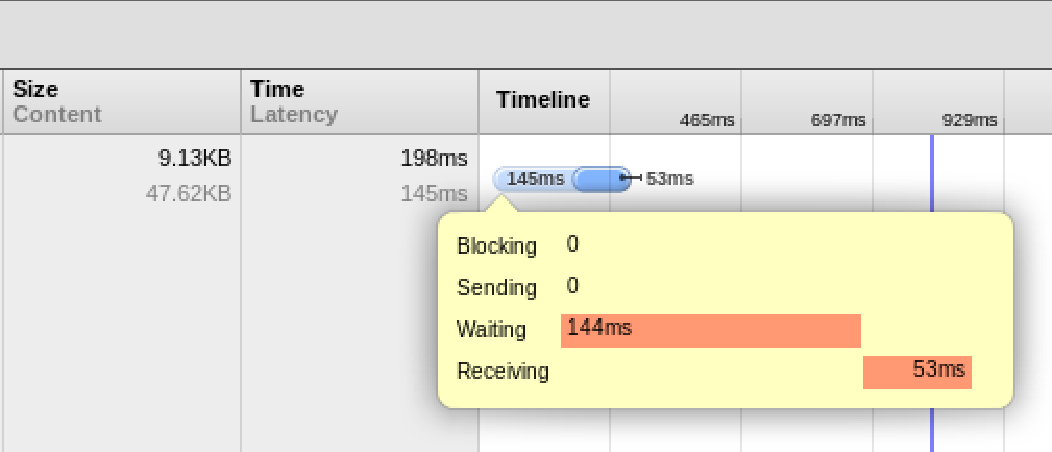
\includegraphics[scale=0.71]{rys1_chrome.pdf}
\end{figure}

Taki spos�b analizy, jest jednak przydatny jedynie w wypadku znacznych problem�w z wydajno�ci� aplikacji, poniewa� testowanie czasu odpowiedzi dla pojedynczego u�ytkownika, wykonuj�cego pojedyncze ��danie, nie jest w �adnym stopniu miarodajne.\\

W celu zapewnienia bardziej rzetelnego testu, nale�y skorzysta� z dedykowanych rozwi�za� takich jak \texttt{ab} oraz \texttt{siege}. 
S� to typowe narz�dzia przeznaczone do sprawdzania jak dobrze serwer radzi sobie z obs�ug� bardziej z�o�onego ruchu sieciowego. 
Przyk�adowo, dla wcze�niej u�ytej strony, mo�na zasymulowa� ruch r�wny wykonaniu 10 jednoczesnych ��da� przez 10 niezale�nych u�ytkownik�w. 
W tym celu nale�y wyda� komend� \lstinline{ab -n 10 -c 10 http://ftims.edu.p.lodz.pl/}. Rezultat dzia�ania komendy widoczny jest na listingu \ref{listing:ab}.

\begin{lstlisting}[caption=Analiza strony z wykorzystaniem narz�dzia \texttt{ab}, label=listing:ab]
Server Software:        Apache/2.2.14
Server Hostname:        ftims.edu.p.lodz.pl
Server Port:            80

Document Path:          /
Document Length:        48759 bytes

Concurrency Level:      10
Time taken for tests:   0.695 seconds
Complete requests:      10
Failed requests:        0
Write errors:           0
Total transferred:      492510 bytes
HTML transferred:       487590 bytes
Requests per second:    14.38 [#/sec] (mean)
Time per request:       695.270 [ms] (mean)
Time per request:       69.527 [ms] (mean, across all concurrent requests)
Transfer rate:          691.77 [Kbytes/sec] received

Connection Times (ms)
              min  mean[+/-sd] median   max
Connect:       52   63   7.4     63      74
Processing:   300  503  90.9    532     632
Waiting:      127  233  62.8    235     381
Total:        354  565  92.9    593     695

Percentage of the requests served within a certain time (ms)
  50%    593
  66%    612
  75%    625
  80%    628
  90%    695
  95%    695
  98%    695
  99%    695
 100%    695 (longest request)

\end{lstlisting}

Jak mo�na wywnioskowa� z powy�szych danych, narz�dzie wykonuje wiele przydatnych analiz, a tak�e wy�wietla informacje o badanym zasobie. 
Wida� przede wszystkim, �e czas oczekiwania na stron� przy 10 u�ytkownikach jest prawie trzykrotnie d�u�szy, ni� podczas jednego ��dania wykonanego w przegl�darce (\ref{fig:rys1_chrome}). 

Oczywi�cie na wyniki pomiar�w ma tak�e wp�yw pr�dko�� po��czenia internetowego, dlatego w celu pomini�cia dodatkowych czynnik�w, testy docelowej aplikacji b�d� wykonywane przede wszystkim na lokalnym serwerze. 
Najbardziej miarodajn� jednostk� okre�laj�c� wydajno�� aplikacji w wypadku narz�dzia \textit{ab} jest liczba zapyta� na sekund� (\textit{req/s}). 
Okre�la ona maksymaln� ilo�� ��da� w jednostce czasu, jak� aplikacja jest w stanie obs�u�y�. Oczywi�cie im wi�ksza warto��, tym lepsza og�lna wydolno�� aplikacji.\\

Na rysunku \ref{fig:rys2_http_lifecycle} przedstawiono cykl �ycia ��dania od u�ytkownika je inicjuj�cego, ko�cz�c na odebraniu odpowiedzi serwera. Jak mo�na zauwa�y� ��danie przebywa stosunkowo d�ug� drog�, nim trafi do faktycznej aplikacji. Wynikiem tego s� dodatkowe op�nienia zale�ne od stopnia skomplikowania architektury trzech pierwszych w�z��w. 
Dlatego te� nale�y mie� na uwadze, �e problemy z szybko�ci� dzia�ania aplikacji nie musz� le�e� wy��cznie po stronie aplikacji lub serwera. 
Do najbardziej popularnych nale��: niska przepustowo�� ��cza internetowego klienta, wolny serwer DNS, daleka lokalizacja geograficzna serwera WWW, �le skonfigurowany router lub bardzo obci��ona sie� lokalna.

\begin{figure}[htbp]
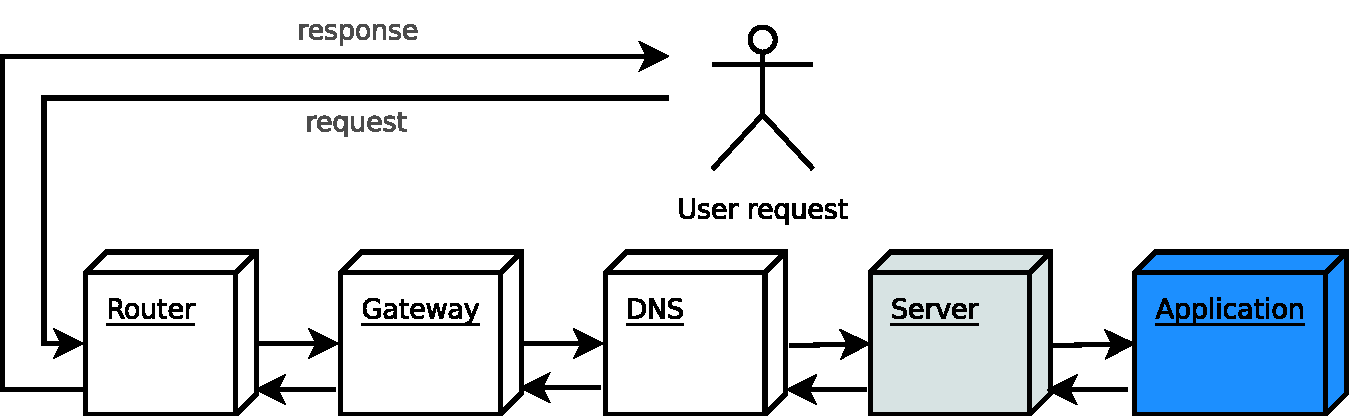
\includegraphics[scale=0.55]{fig_request.pdf}
\caption{Cykl �ycia ��dania}
\label{fig:rys2_http_lifecycle}
\end{figure}

Nawi�zuj�c do listingu \ref{listing:ab}, warto�ciami zwi�zanymi ze wspomnianymi w poprzednim akapicie w�z�ami s� \texttt{Connect} oraz \texttt{Waiting}, czyli odpowiednio czas oczekiwania na po��czenie z zasobem i czas pobierania odpowiedzi z zasobu. Istnieje 5 g��wnych czynnik�w wp�ywaj�cych na czas odpowiedzi serwera.

\begin{description}

\item[Po�o�enie geograficzne i problemy z sieci� komputerow�.]

Nie bez znaczenia dla czasu odpowiedzi, jaki u�ytkownik odczuwa jest te� lokalizacja serwer�w stron. Je�li serwery s� zlokalizowane w USA, a u�ytkownicy odwiedzaj�cy stron� s� np. z Europy, dystans jaki musi pokona� ��danie od momentu dotarcia do zasobu, oczekiwania, a� do jego pobrania jest nie wsp�miernie wi�kszy ni� w wypadku stron hostowanych dla tego samego po�o�enia geograficznego. 
Stopie� op�nienia jest zazwyczaj uzale�niony od ilo�ci router�w, serwer�w po�rednich, a nawet ocean�w, kt�re pokonuje ��danie od punktu pocz�tkowego do odbiorcy i z powrotem.

\item[Wielko�� dokumentu odpowiedzi serwera.] Zale�no�� mi�dzy wielko�ci� dokumentu, a czasem odpowiedzi serwera jest oczywista, �atwo wi�c sprawdzi�, �e im wi�kszy dokument trzeba pobra�, tym wi�cej czasu potrzeba na zako�czenie tego procesu.

\item[Wykonywanie kodu aplikacji.] Najcz�stsza przyczyna wolnego dzia�ania aplikacji wynika w�a�nie z braku optymalizacji kodu klienta. D�ugi czas wykonywania kodu aplikacji implikuje, d�ugi czas ��czny oczekiwania na odpowied� serwera. Problem ten zostanie szczeg�owiej poruszony w rozdziale \ref{cha:optymalizacja_aplikacji}.

\item[Rodzaj u�ytej przegl�darki.] Nie bez znaczenia dla og�lnego czasu �adowania strony jest r�wnie� rodzaj u�ytej przegl�darki. Cz�sto wbudowane w przegl�dark� wewn�trzne mechanizmy buforowania zasob�w pozwalaj� w znaczny spos�b zredukowa� ilo�� zapyta� wysy�anych do serwera. Dotyczy to zw�aszcza danych statycznych takich jak arkusze CSS, pliki JavaScript czy zasoby graficzne, kt�re nie zmieniaj� si� zbyt cz�sto. 

\item[Konfiguracja serwera WWW.] W zale�no�ci od u�ytej technologii, istnieje wiele r�nych serwer�w HTTP. W�r�d najcz�ciej u�ywanych, prym wiedzie serwer HTTP \textit{Apache}. 
Dla rozwi�za� napisanych w technologii Java cz�sto wykorzystywane s� serwery \textit{GlassFish}, \textit{Tomcat}, \textit{Jetty}. W wi�kszo�ci wypadk�w zaraz po instalacji, oprogramowanie serwera nie nadaje si� jeszcze do wykorzystania w produkcji. 
Nale�y wywa�y� ustawienia serwera do bie��cych potrzeb, poniewa� w wi�kszo�ci wypadk�w domy�lne ustawienia mog� znacznie obni�y� og�ln� wydajno��. 
Innym wa�nym dzia�aniem jest dostosowywanie serwera do konkretnych zastosowa� - do serwowania plik�w statycznych lepszym rozwi�zaniem jest wykorzystanie bardziej oszcz�dnego pami�ciowo i operacyjnie serwera \textit{Ngnix}, natomiast do bardziej zaawansowanych zastosowa�, w tym wykonywanie kodu aplikacji, serwera Apache lub osobnej instancji serwera \textit{Ngnix}.

\end{description}

Administratorzy serwer�w WWW maj� bezpo�redni dost�p do statystyk odwiedzalno�ci stron, przez co pozwala to zaobserwowa� pewne trendy odwiedzin u�ytkownik�w. 
Cz�sto jest tak, �e dane zasoby s� du�o intensywniej odpytywane przez u�ytkownik�w np. w czasie 10 minut stron� odwiedza 100 u�ytkownik�w. 
�atwo to sobie wyobrazi� np. w wypadku premiery jakiej� nowej gry, lub publikacji wynik�w egzaminu na uczelni. 
Taki periodyczny, lecz bardzo wzmo�ony ruch mo�e powodowa� pewne trudne do ustalenia problemy z dzia�aniem aplikacji. Dlatego te� tw�rcy narz�dzia \texttt{ab}, zaimplementowali r�wnie� mo�liwo�� test�w czasowych (ang. \textit{timed tests}). W ten spos�b mo�na zasymulowa� jak strona b�dzie si� zachowywa�a r�wnie� w takich nag�ych wypadkach.\\

Wydaj�c komend� \lstinline{ab -c 10 -t 30 http://ftims.edu.p.lodz.pl/}, mo�na sprawdzi�, jak zachowa si� aplikacja odwiedzana przez 10 u�ytkownik�w jednocze�nie w czasie 30 sekund. Ta komenda pozbawiona jest parametru \textit{-t ilo�� ��da�}, oznacza to �e symulacja zako�czy si� po 30 sekundach lub po osi�gni�ciu limitu 50 000 ��da�.

\begin{lstlisting}[caption=Test obci��enia czasowego, label=listing:ab_2]
Benchmarking ftims.edu.p.lodz.pl (be patient)
Finished 504 requests

Server Software:        Apache/2.2.14
Server Hostname:        ftims.edu.p.lodz.pl
Server Port:            80

Document Path:          /
Document Length:        48759 bytes

Concurrency Level:      10
Time taken for tests:   40.180 seconds
Complete requests:      504
Failed requests:        0
Write errors:           0
Total transferred:      24822504 bytes
HTML transferred:       24574536 bytes
Requests per second:    12.54 [#/sec] (mean)
Time per request:       797.213 [ms] (mean)
Time per request:       79.721 [ms] (mean, across all requests)
Transfer rate:          603.31 [Kbytes/sec] received

Connection Times (ms)
              min  mean[+/-sd] median   max
Connect:       48   65  14.3     61     145
Processing:   284  436 288.9    376    2957
Waiting:      119  199 281.5    151    2660
Total:        333  500 287.8    439    3007

Percentage of the requests served within a certain time (ms)
  50%    439
  66%    458
  75%    477
  80%    493
  90%    563
  95%    666
  98%   1420
  99%   2142
 100%   3007 (longest request)

\end{lstlisting}

Listing \ref{listing:ab_2} przedstawia wynik test�w czasowych. Najwa�niejsz� informacj� z punktu widzenia optymalizacji jest ilo�� ��da� na sekund�, kt�ra w tym wypadku wynosi \texttt{12.54}. Narz�dzie \texttt{ab} pozwala r�wnie� zdiagnozowa� potencjalne b��dy aplikacji pod wp�ywem zbyt du�ego ruchu. 
Pola takie jak \texttt{Failed requests} oraz \texttt{Write errors} u�atwiaj� okre�lenie prawid�owo�ci wykonywania ��da�. W powy�szym przyk�adzie, warto�ci s� akceptowalne (�redni czas ��dania to 0.5 sekundy), co najwa�niejsze nie wyst�puj� b��dy na poziomie serwera WWW i z du�ym prawdopodobie�stwem r�wnie� na poziomie aplikacji. Oczywi�cie zauwa�alny jest spadek wydajno�ci, w por�wnaniu z pierwszym testem, co prawda warto�ci �rednie s� zbli�one, jednak wida� wi�ksze rozbie�no�ci mi�dzy warto�ciami minimalnymi a maksymalnymi. Najd�u�sze zapytanie zaj�o ponad 3 sekundy. 

W dokumentacji aplikacji \texttt{ab}, mo�na znale�� informacj�, �e niekt�re serwery mog� blokowa� wysy�ane przez niego nag��wki HTTP. 
W tym celu mo�na wykorzysta� prze��cznik umo�liwiaj�cy podanie si� za inn� przegl�dark�. 
Np. chc�c zasymulowa� odwiedziny przy u�yciu przegl�darki Chrome nale�y wykona� poni�sz� komend�.
\lstinline{ab -n 100 -c 5 -H "Mozilla/5.0 (Windows; U; Windows NT 5.1; en-US) AppleWebKit/534.2 (KHTML, like Gecko) Chrome/6.0.447.0 Safari/534.2" http://www.example.com}.\\

Pomimo wielu zalet wynikaj�cych z korzystania z narz�dzia \texttt{ab}, istnieje jedna zasadnicza wada. Aplikacja nie daje mo�liwo�ci przetestowania pewnego scenariusza lub jest to bardzo niewygodne, a przypadku aplikacji z wykorzystaniem technologii \textit{JavaScript} i \textit{AJAX} wr�cz niewykonalne.

Dlatego te� na prze�omie lat wyspecjalizowa�y si� bardziej zaawansowane narz�dzia przeznaczone do prze�ledzenia logicznej kolejno�ci dzia�a� wykonywanych na stronie (pewnego przypadku u�ycia) i wykonywanie analiz w�a�nie w ramach logicznego zbioru akcji. W ten spos�b mo�liwe jest przeprowadzenie tzw. \textit{test�w funkcjonalnych}, a tak�e sprawdzenie w jakim stopniu s� one wra�liwe na zwi�kszony ruch sieciowy. 

Jednym z przyk�ad�w takiego narz�dzia o naprawd� olbrzymich mo�liwo�ciach jest \textit{Apache JMeter}. Z jego pomoc� mo�liwe jest nagranie pewnego ci�gu akcji wykonanych przy pomocy przegl�darki, a nast�pnie przeprowadzenie ci�gu analiz i test�w na tak wyodr�bnionym zbiorze. Tabela \ref{table:1_jmeter} pokazuje wynik dzia�ania przyk�adowego scenariusza polegaj�cego na symulowaniu wej�cia na stron� \texttt{http://www.wp.pl}, a nast�pnie klikni�ciu jednego z link�w wiadomo�ci, po czym klikni�ciu na kolejny link z dost�pnych na bie��cej stronie. Ostatnim elementem �a�cucha akcji jest wys�anie komentarza do artyku�u. JMeter podobnie jak \texttt{ab} umo�liwia wykonywanie r�wnoleg�ych po��cze� u�ytkownik�w okre�lanych jako w�tki (\textit{threads}).\\

W zdefiniowanym przypadku u�ycia 5 u�ytkownik�w wykonuje jednocze�nie t� logik� 500 razy. Na zako�czenie dane mo�liwe s� do wyeksportowania do formatu \textit{CSV} lub wy�wietlone bezpo�rednio na ekranie. JMeter jest narz�dziem bardzo rozbudowanym, przez co idealnie nadaje si� do testowania zaawansowanych scenariuszy zar�wno pod k�tem poprawno�ci dzia�ania, jak r�wnie� og�lnej wydajno�ci.

\begin{table}\centering
\ra{1.3}
\begin{tabular}{@{}rrrrcrrrcrrr@{}}\toprule
URL & �rednia & Min & Max & B��d (\%) & Req/Min \\
\bottomrule
..14543704,wiadomosc.html & 2299 & 415 & 94329 & 2.2 & 43.7 \\  
...1028235,wiadomosci.html & 2485 & 335 & 94434 & 2.8 & 43.7 \\  
...14545325,wiadomosc.html & 2023 & 394 & 94285 & 1.8 & 43.7 \\  
\bottomrule
\textbf{��cznie} & \textbf{2269} & \textbf{335} & \textbf{94434} & \textbf{2.27} & \textbf{131.1} \\  
\end{tabular}
\caption{Tabela z rezultatem dzia�ania aplikacji JMeter}
\label{table:1_jmeter}
\end{table}

\section{Analiza wydajno�ci frontendu}

W poprzednim podrozdziale zosta�a om�wiona tematyka testowania czasu dzia�ania zasob�w serwowanych przez serwer WWW. Wykorzystuj�c wspomniane wcze�niej narz�dzia mo�na jednoznacznie ustali� czy aplikacja funkcjonuje w spos�b prawid�owy, czy nie wyst�puj� b��dy w pracy serwera oraz jak dobrze oprogramowanie radzi sobie ze wzmo�onym obci��eniem.

Wydawa� by si� mog�o, �e problem testowania wydajno�ci aplikacji zosta� jednoznacznie om�wiony.
Nic bardziej mylnego, jedynie w idealnym �wiecie, strona WWW sk�ada�a by si� wy��cznie z tekstu, a u�ytkownicy do przegl�dania Internetu, korzystaliby wy��cznie z terminali.\\


Wsp�czesny u�ytkownik internetu, do przegl�dania jego zasob�w wykorzystuje przegl�dark� internetow�, zdoln� do wy�wietlania zar�wno tekstu, jak i medi�w wszelakiego typu. Dlatego  te�, dla wi�kszej precyzji, konieczne jest wyszczeg�lnienie kluczowego komponentu oprogramowania, jakim jest \textit{front-end} aplikacji. 

W przypadku aplikacji internetowych, \textit{front-end} to graficzny interfejs s�u��ca do komunikacji u�ytkownika ze stron� i prezentacji danych opracowanych przez zaplecze systemu (back-end) w spos�b przyst�pny i zrozumia�y.\\
 
Odpowiednia optymalizacja \textit{front-endu} jest o tyle wa�na, �e jest to pierwsza technologia z jak� u�ytkownik ma kontakt w momencie korzystania z  aplikacji webowej \cite{book:proPHP}.

Frontend realizuje  przetwarzanie i analiz� wyniku odpowiedzi serwera, przy czym obowi�zuj�cym j�zykiem komunikacji jest j�zyk HTML (\textit{HiperText Markup Language }). Od kilku lat w wyniku rozwoju trendu WEB 2.0, istotnym zabiegiem, projektowanych aplikacji, staje si� przeniesienie cz�ci logiki na stron� przegl�darki (frontendu). Cienkie do tej pory aplikacje webowe (\textit{thin client}), zaczynaj�  - dzi�ki zdobycz� technologicznym takim jak \textit{AJAX} realizuj� znacznie szerszy zakres funkcjonalny ni� dotychczas. Oznacza to, �e przetwarzanie danych mo�e mie� miejsce wykorzystuj�c przegl�dark� internetow� i j�zyk JavaScript. Dlatego te� kolejnym istotnym elementem analizy wydajno�ciowej staje si� analiza \textit{frontendu}.\\


Na podstawie bada� firmy Juniper, stwierdzono, �e �redni czas, jaki u�ytkownik jest w stanie poczeka� na za�adowanie strony to zaledwie 4 sekundy. Nie warto wi�c traci� potencjalnych klient�w strony, tylko i wy��cznie z powodu braku optymalizacji po stronie przegl�darki.

W�r�d istniej�cych na rynku rozwi�za� s�u��cych do analizy po stronie klienta, najpopularniejszymi s� te, kt�re s� wbudowane bezpo�rednio w interfejs przegl�darki internetowej (jest to przecie� najbardziej intuicyjne podej�cie). Jednym z pierwszych rozwi�za� tego typu by�a wtyczka \texttt{Firebug} napisana dla przegl�darki Firefox. Jest to obecnie najbardziej zaawansowane narz�dzie tego typu, rywalizuj�ce jednocze�nie z natywnymi dodatkami deweloperskimi dla przegl�darki Chrome.\\

Interfejs Firebuga pozwala na szczeg�ow� inspekcj� kodu HTML wraz z mo�liwo�ci� dynamicznej operacji na w�z�ach DOM dokumentu HTML. Nie mniej wa�nymi narz�dziami s�: mo�liwo�� wykonywania i debugowania kodu JavaScript na stronie, inspekcja zwi�zanego z dokumentem HTML obiektu DOM, edycja i rewizja kodu JavaScript oraz narz�dzie do monitorowania ruchu sieciowego wykonywanego przez aplikacj�.

Ten ostatni modu� pe�ni podobn� rol� do narz�dzia \texttt{ab}, jednak wy�wietla wszystkie zasoby, kt�re maj� bezpo�rednie powi�zanie z bie��cym dokumentem HTML. Omawiane wcze�niej narz�dzia pokazywa�y jedynie czas renderowania dokumentu HTML, jednak nale�y mie� na uwadze, �e strona internetowa sk�ada si� z wielu r�nych zasob�w, w�r�d kt�rych nie spos�b pomin��: grafik, arkuszy CSS, kodu JavaScript, aplet�w Java czy obiekt�w Adobe Flash.

Ka�da strona mo�e zawiera� zr�nicowan� ilo�� takich zasob�w, dlatego na ��czny czas �adowania strony sk�ada si� zar�wno czas oczekiwania na dokument HTML, jak r�wnie� czas konieczny na pobranie ka�dego z powi�zanych z nim zasob�w. 

Nawi�zuj�c do \cite{book:yahoo} istniej zasada, kt�ra m�wi, �e tylko 10-20\% czasu odpowiedzi jest sp�dzane na oczekiwanie dokumentu HTML, natomiast pozosta�e 80-90\% to czas na pobieranie pozosta�ych zasob�w i �adowanie zawarto�ci DOM.

Rysunek \ref{fig:ruch_sieciowy} jest najlepszym przyk�adem tej zasady. Strona wykonuje 32 zapytania do serwera, z czego tylko jedno to ��danie dokumentu HTML. Pobranie tego dokumentu zaj�o oko�o 400ms, tymczasem ��czny czas wczytywania strony wyni�s� \textbf{3.21 sekundy}. Oznacza to, �e generowanie dokumentu zaj�o zaledwie \textbf{12\%} ��cznego czasu oczekiwania. 

Na podstawie danych z Firebuga �atwo stwierdzi� pewne nieprawid�owo�ci, bowiem w ramach strony wczytywane s� 2 stosunkowo du�e (1,1 MB) dokumenty graficzne, kt�re prawdopodobnie nie zosta�y wymiarowane do odpowiednich rozmiar�w. \texttt{Firebug} stanowi, wi�c cenne narz�dzie przy diagnostyce \textit{frontendu} strony. Narz�dzie sstaje si� jeszcze przydatniejszy przy pojawianiu si� element�w dynamicznych JavaScript, poniewa� pozwala �ledzi� zar�wno aktualnie wykonywany kod, jak r�wnie� nas�uchiwa� zapyta� asynchronicznych wykonywanych przez AJAX. Narz�dzie to mo�e by� r�wnie� przydatne podczas �ledzenia zmian dokonywanych w dokumencie HTML, za pomoc� narz�dzia inspekcji, umo�liwia bowiem zbadanie ka�dego w�z�a.

\begin{figure}[hbtp]
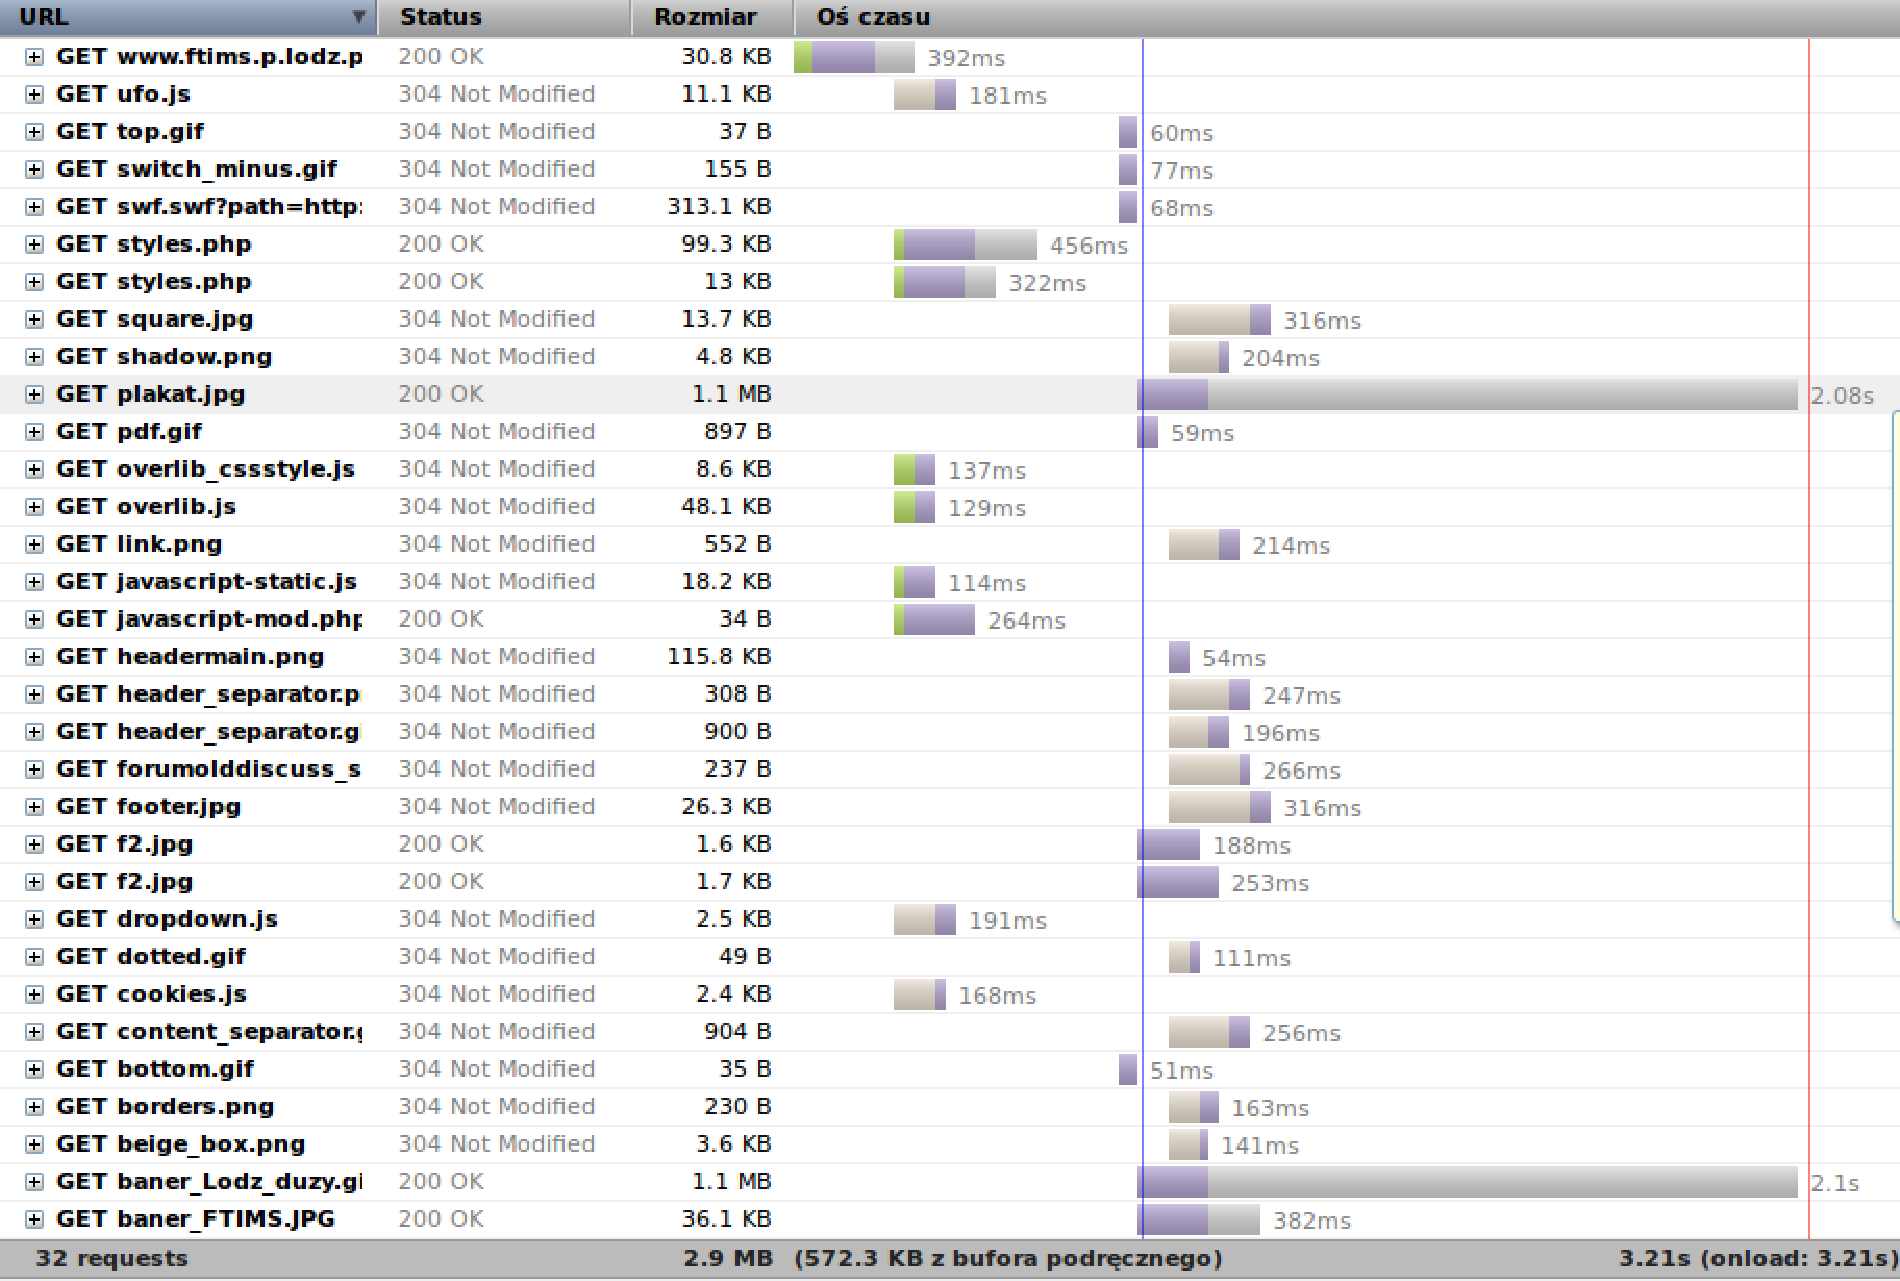
\includegraphics[scale=0.45]{rys3_firebug.pdf}
\caption{Analiza ruchu sieciowego na stronie http://ftims.p.lodz.pl}
\label{fig:ruch_sieciowy}
\end{figure}

\section{Analiza wydajno�ci bazy danych}

Bardzo cz�sto og�lna wydajno�� aplikacji uzale�niona jest od szybko�ci operacji odczytu / zapisu bazy danych. W pewnym momencie tw�rcy aplikacji zaczynaj� oczekiwa� od niej wi�kszej wydajno�ci. Nale�y jednak zada� pytanie co nale�y tak naprawd� optymalizowa�? Konkretne zapytanie? Schemat bazy? Czy mo�e sprz�t na kt�rym baza danych pracuje? Jedynym sposobem na znalezienie jednoznacznej odpowiedzi, jest zmierzenie pracy wykonywanej przez baz�  i sprawdzenie wydajno�ci pod wp�ywem r�nych czynnik�w \cite{book:mysql}.

Bazy danych ewoluowa�y na przestrzeni kilkunastu lat, pocz�tkowo by�y to po prostu pliki o okre�lonej strukturze, jednak wraz ze wzrostem wymaga� zacz�to stosowa� r�wnoleg�y dost�p do danych, a tak�e dbaj�c o sp�jno�� danych, zaimplementowano system transakcji.

Obecnie wida� specjalizacji baz danych do konkretnych zastosowa�, pomimo dominacji na rynku baz relacyjnych opartych o standard \textit{SQL 93}, zacz�to r�wnie� torowa� drog� nowym rozwi�zaniom takim jak \textit{NoSQL} czyli bazy danych o nieuporz�dkowanej strukturze, pozbawionych �ci�le zdefiniowanych schemat�w, zyskuj�c wi�ksz� elastyczno��. Dodatkowo w okre�lonych zastosowaniach tego typu bazy danych okazuj� si� du�o szybsze ni� bazy relacyjne. Szybko�� ta jest tym wi�ksza, im wi�ksza jest przechowywana kolekcja danych. S� to, wi�c bazy wysoce skalowalne, cho� mniej sp�jne ni� standardowe.\\

W�r�d system�w bazodanowych wykorzystywanych w aplikacji e-commerce, bardzo du�� popularno�ci� cieszy si� oprogramowania MySQL. Pomimo du�o mniejszych mo�liwo�ci ni� np. komercyjne rozwi�zania Oracle czy MS SQL Server, omawiana baza danych jest elastyczna i �atwo zaadaptowa� j� do w�asnych potrzeb. Od czasu wprowadzenia zgodno�ci ze standardem ACID, MySQL zacz�� by� szeroko wykorzystywany w e-biznesie. 

\begin{figure}[hbtp]
\center
\caption{Schemat architektury MySQL}
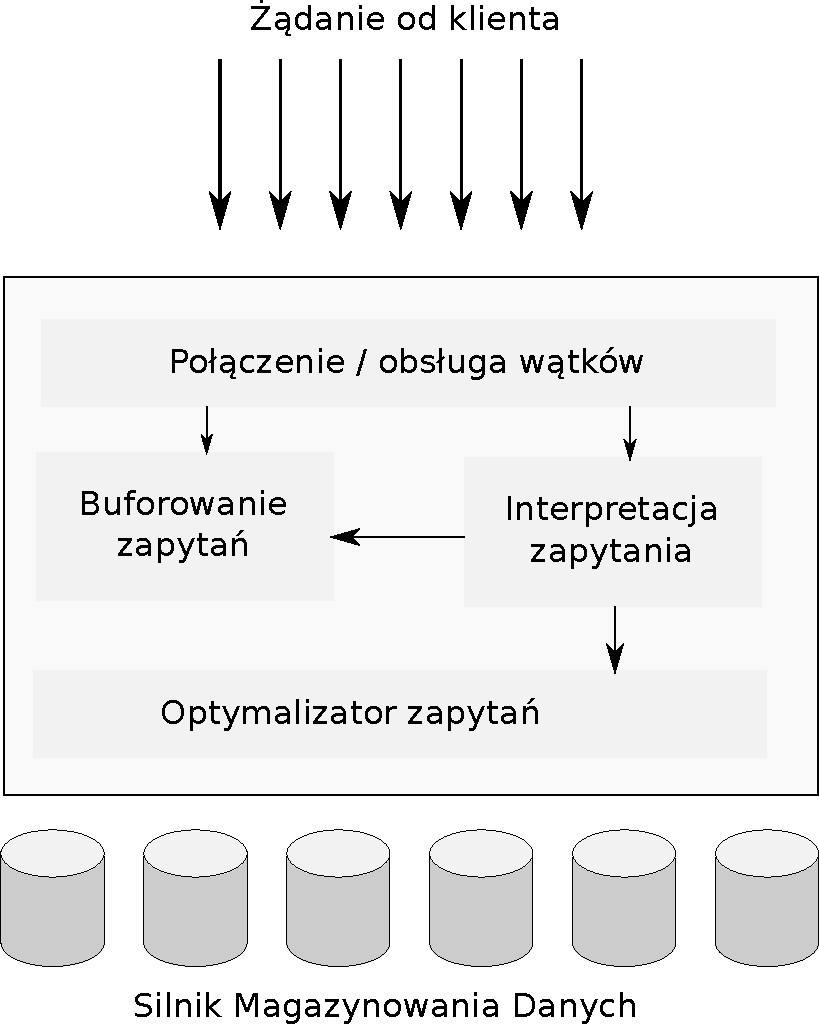
\includegraphics[scale=0.5]{baza.pdf}
\label{fig:mysql_schemat}
\end{figure}

Rysunek \ref{fig:mysql_schemat} przedstawia, jak wygl�da architektura systemu baz danych MySQL, z punktu widzenia funkcjonalny komponent�w \cite{book:proPHP}[str. 26]. Pierwsza warstwa zawiera us�ugi, kt�re wbrew pozorom nie s� unikalne tylko dla omawianego oprogramowania. S� to us�ugi  charakterystyczne dla wi�kszo�ci narz�dzi w architekturze sieciowej. Wyr�niono wi�c obs�ug� po��czenia, uwierzytelnianie itd.
Druga warstwa wprowadza wiele zmian i komponent�w specyficznych dla MySQL'a. Wyr�niamy wi�c komponenty odpowiedzialne za parsowanie zapyta�, a tak�e ich optymalizacj�, buforowanie oraz kod odpowiedzialny za implementacje wbudowanych funkcji (np. data, czas, funkcje matematyczne i kryptograficzne). Ka�da funkcjonalno�� oferowana przez kt�rykolwiek z silnik�w sk�adowania danych (\textit{storage engine}), ma tu swoje miejsce (np. procedury u�ytkownika, wyzwalacze oraz widoki).

Trzecia warstwa wyr�nia wszystkie silniki sk�adowania, kt�re odpowiedzialne s� bezpo�rednio za przechowywanie i pobieranie danych w MySQL'u. Ka�dy z silnik�w, ma r�ne zastosowania (podobnie jak r�ne systemy plik�w w systemach operacyjnych). Komunikacja z ka�dym z nich odbywa si� wykorzystuj�c wewn�trzne API. Wspomniany interfejs ukrywa r�nice w specyfice ka�dego z mechanizm�w, przez co zapytania s� bardziej abstrakcyjne i prostsze w u�yciu dla u�ytkownika ko�cowego. Podobnie jak w wypadku serwer�w WWW, mi�dzy mechanizmem sk�adowania a serwerem MySQL wyst�puje zale�no��: ��danie - odpowied�. Oznacza to, �e serwer wysy�a ��danie i oczekuje na odpowied�.

Najlepsz� strategi� optymalizacji, jest szukanie miejsc aplikacji, kt�re dzia�aj� najwolniej. Utworzono nast�puj�cy schemat bazy danych (rys. \ref{fig:baza_danych_test}). Na podstawie rysunku wida� zale�no�� studenta, kt�ry przynale�y do 1 profilu (nauczyciela), kt�ry z kolei nale�y do organizacji. Podobnie student mo�e nale�e� do jednego z istniej�cych kampus�w.

\begin{figure}[hbtp]
\center
\caption{Schemat testowej bazy danych}
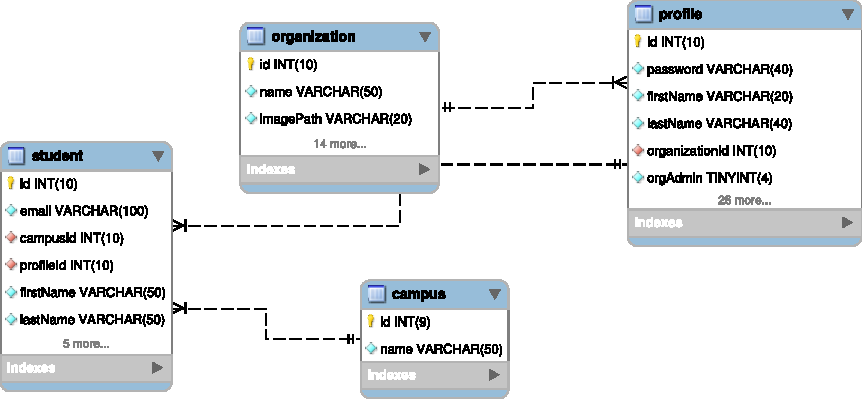
\includegraphics[scale=1]{baza_test.pdf}
\label{fig:baza_danych_test}
\end{figure}

Jak zachowa si� baza danych przy pr�bie stworzenia alfabetycznego indeksu student�w, kt�rych nazwiska zaczynaj� si� na dan� liter� (listing \ref{listing:sql})?

\begin{lstlisting}[language=sql, caption=Zapytanie do wy�wietlenia menu ksi��ki adresowej uczni�w, label=listing:sql]
SELECT left(s.lastName, 1) letter, COUNT(s.id) students
FROM student s 
WHERE s.lastName > 'A'
GROUP BY letter
\end{lstlisting}

Rezultat dzia�ania zapytania SQL widoczny jest na listingu \ref{listing:sql_adresowa}. Jak wida�, zapytanie wykonuje si� w czasie 40 milisekund. Jest to dosy� kr�tko, ale wynika to z g�ownie z rozmiar�w kolekcji danych (20244 student�w). Wraz z rozrastaniem si� tej tabeli, czas potrzebny na wykonanie tego zapytania b�dzie si� systematycznie powi�ksza�. Dzieje si� tak, poniewa� tabela student�w nie posiada �adnego indeksu.

\begin{lstlisting}[caption=Wynik zapytania z listingu \ref{listing:sql}, label=listing:sql_adresowa]
+--------+----------+
| letter | students |
+--------+----------+
| A      |      999 |
| B      |     1749 |
| C      |      814 |
| D      |      670 |
| E      |      385 |
| F      |      918 |
| G      |     1599 |
| H      |      808 |
| I      |      245 |
| J      |      194 |
| K      |     1695 |
| L      |     1156 |
| M      |     1411 |
| N      |      492 |
| O      |      240 |
| P      |      686 |
| Q      |       14 |
| R      |     1259 |
| S      |     2662 |
| T      |      499 |
| U      |       57 |
| V      |      244 |
| W      |      698 |
| Y      |      316 |
| Z      |      400 |
+--------+----------+
25 rows in set (0.04 sec)

\end{lstlisting}

\subsubsection{Czym jest indeks?}

\textit{Indeks} jest struktur� danych przeznaczon� do pomocy systemowi baz danych w efektywnym pobieraniu informacji z tabel. S� one cz�sto wymagane dla zapewnienia dobrej wydajno�ci. Indeksy s� szczeg�lnie wa�ne w momencie kiedy baza danych si� rozrasta, poniewa� ilo�� element�w do przeszukiwania wierszowego ulega zwielokrotnieniu.

Podczas zwyk�ego wyszukiwania warto�ci w bazie danych, program musi przeszuka� ka�d� kolumn�, ka�dego wiersza w poszukiwaniu okre�lonej warto�ci. W wypadku indeks�w sprawa jest uproszczona poniewa� dysponujemy pewnym podzbiorem warto�ci np. z danej kolumny lub wyra�enia. W ten spos�b silnik bazy danych wie, �e dana warto�� znaleziona w okre�lonym indeksie powi�zana jest z okre�lonym rekordem, wi�c odpowied� jest b�yskawiczna.

Oczywi�cie wykorzystywanie indeks�w wi��e si� r�wnie� z pewn� zaj�to�ci� danych, poniewa� opr�cz danych w tabeli, trzeba dodatkowo przechowywa� dane indeks�w. Przeliczaj�c jedna zyski do strat, wi�kszo�� przemawia jednak za stosowaniem indeks�w.

\subsection{Optymalizacja table przy u�yciu indeks�w}

Optymalizacja zapyta� przy u�yciu indeks�w jest stosunkowo prosta i polega na stworzeniu indeksu, kt�ry najlepiej pasuje do wyszukiwanej zawarto�ci. W naszym wypadku potrzeba indeksu przechowuj�cy pierwsz� liter� nazwiska. Z drugiej strony sortowanie po nazwisku lub nawet wyszukiwanie po nim jest do�� cz�st� operacj� dlatego warto stworzy� kompletny indeks dla pola \texttt{lastName} tabeli student (\ref{fig:baza_danych_test}). Na podstawie wyniku uzyskanego w listingu \ref{listing:sql_adresowa2}, wida� znaczn� popraw� czasu wykonywania. Wszystkie zapytania wykorzystuj�ce kolumn� \texttt{lastName}, powinny wykonywa� si� zdecydowanie szybciej. 

\begin{lstlisting}[caption=Utworzenie indeksu na polu nazwiska dla tabeli student]
ALTER TABLE `student` ADD INDEX `lastName_idx`(`lastName`);
\end{lstlisting}

\begin{lstlisting}[caption=Wynik zapytania z listingu \ref{listing:sql} po optymalizacji indeksu, label=listing:sql_adresowa2]
+--------+----------+
| letter | students |
+--------+----------+
| A      |      999 |
| B      |     1749 |
| C      |      814 |
| D      |      670 |
| E      |      385 |
| F      |      918 |
| G      |     1599 |
| H      |      808 |
| I      |      245 |
| J      |      194 |
| K      |     1695 |
| L      |     1156 |
| M      |     1411 |
| N      |      492 |
| O      |      240 |
| P      |      686 |
| Q      |       14 |
| R      |     1259 |
| S      |     2662 |
| T      |      499 |
| U      |       57 |
| V      |      244 |
| W      |      698 |
| Y      |      316 |
| Z      |      400 |
+--------+----------+
25 rows in set (0.01 sec)

\end{lstlisting}

\subsubsection{Kolejno�� z��cze�}

Z��czenia (ang. \textit{joins}), s� operacj� spajaj�c� ze sob� dwie lub wi�cej tabel. Dopuszczalne s� ��czenia 2 r�nych tabel lub tej samej (\textit{self-joins}). U�ywanie z��cze� wynika w du�ej mierze z normalizacji bazy danych, a co za tym idzie usuni�cia nadmiarowo�ci z rekord�w tabel. Takie podej�cie w du�ej mierze poprawia sp�jno�� danych, ale r�wnie� mo�e pogorszy� w du�ej mierze wydajno�� zapyta�.\\

Standard ANSI wyr�nia 4 rodzaje z��cze�: INNER, OUTER, LEFT, RIGHT. W specjalnych okoliczno�ciach tabela mo�e by� r�wnie� po��czona sama ze sob�. Zasadnicza r�nica w specyfice polega na kryterium ��czenia - w wypadku \textit{INNER JOIN�W} wymagane jest istnienie odpowiadaj�cych sobie krotek po dw�ch stronach relacji, natomiast \textit{OUTER JOIN} wymaga spe�nienia tego kryterium przynajmniej na jednej ze strony relacji - odpowiednio lewej lub prawej. 

R�nice mi�dzy z��czeniami przek�adaj� si� r�wnie� na wydajno�� dzia�ania, najpopularniejsze ze z��cze� \textit{inner join'y} s� najszybsze, podczas, gdy pozosta�e przeznaczone s� do bardziej specyficznych zastosowa�.

Kolejny z przeprowadzanych test�w, b�dzie polega� na z��czeniu ze sob� student�w oraz profili, innymi s�owy wy�wietleniu wszystkich student�w przynale�nych do kt�rego� z profili. Wynik dzia�ania poszczeg�lnych test�w (listing \ref{listing:zapytania_profile}) zosta� zestawiony w tabeli \ref{table:3_sql}. Wyniki zapyta� stanowi� potwierdzenie og�lnie przyj�tych zasad optymalizacji zapyta�, \textit{inner join} okaza� si� najszybszym ze z��cze�, jednocze�nie wida�, �e kolejno�� wykonywania z��cze� r�wnie� ma wp�yw na wydajno��. Zazwyczaj powinno si� zaczyna� od tabeli, kt�ra posiada miej rekord�w (w tym wypadku tabela profile). Ogromna r�nica mi�dzy czasem wykonywania \textit{left joina} oraz \textit{right joina} w odwrotnej kolejno�ci ��czenia wynika z braku indeksu dla pola \texttt{profileId} tabeli \texttt{student}. Po dodaniu indeks�w wida� 10-krotn� popraw� szybko�ci wykonywania tego zapytania.\\

Przedstawione dotychczas przypadki by�y stosunkowo proste do naprawy, cz�sto jednak zapytania s� du�o bardziej rozbudowane i ci�kie do szybkiej dekompozycji. Warto wtedy skorzysta� z udost�pnianego przez MySQL narz�dzia \texttt{EXPLAIN}. Oferuje on pomoc w zakresie dekompozycji bardziej skomplikowanych zapyta�. Narz�dzie to pokazuje m.in wykorzystane klucze dla ��cze�, liczebno�� ��czonych tabel, proponowane usprawnienia indeks�w.

\begin{lstlisting}[caption=Kilka mo�liwych do wykorzystania zapyta�,label=listing:zapytania_profile]
SELECT SQL_NO_CACHE * FROM profile p inner join student s on s.profileId = p.id
SELECT SQL_NO_CACHE * FROM profile p left join student s on s.profileId = p.id
SELECT SQL_NO_CACHE * FROM profile p right join student s on s.profileId = p.id

SELECT SQL_NO_CACHE * FROM student s inner join profile p on s.profileId = p.id
SELECT SQL_NO_CACHE * FROM student s left join profile p on s.profileId = p.id
SELECT SQL_NO_CACHE * FROM student s right join profile p on s.profileId = p.id
\end{lstlisting}

\begin{table}\centering
\ra{1.3}
\begin{tabular}{@{}rrrrcrrrcrrr@{}}\toprule
Typ & Czas wykonywania [sec] & Ilo�� rekord�w \\
\bottomrule
\texttt{inner join student} & 0.2557 & 20244\\
\texttt{left join student}  & {\color{red}\textbf{5.2125 / 0.5635}} & 20463\\
\texttt{right join student} & 0.2634 & 20244\\
\bottomrule
\texttt{inner join profile} & 0.2726 & 20244\\
\texttt{left join profile}  & 0.3272 & 20463\\
\texttt{right join profile} & {\color{red}\textbf{5.2236 / 0.5704}} & 20463
\end{tabular}
\caption{Tabela z rezultatem dzia�ania poszczeg�lnych zapyta�}
\label{table:3_sql}
\end{table}

Jednym z zapyta�, kt�re mo�e stanowi� potencjalny problem w analizie jest zapytanie zaczerpni�te z istniej�cej aplikacji opartej o przedstawiony na rysunku \ref{fig:baza_danych_test} schemat bazy danych. Przedstawione na listingu \ref{listing:sql_dlugie} zapytanie s�u�y do pokazania warto�ci sum w poszczeg�lnych aktywno�ciach takich jak programy studenckie, praktyki, ilo�� student�w itp. Zapytanie to jest wykonywane w kontek�cie okre�lonego roku szkolnego, a tak�e konkretnej organizacji - wy�wietla warto�ci dla podleg�ych kampus�w.

\begin{lstlisting}[caption=Bardziej rozbudowane zapytanie SQL, language=SQL, label=listing:sql_dlugie]
SELECT
c.id, c.name,

(select count(s5.id)
from student s5
inner join profile p2 on p2.id = s5.profileId
left join profileCampus pc2 on pc2.profileId = p2.id
left join organizationCampus oc2 on oc2.organizationId = p2.organizationId    
       where (oc2.campusId = c.id or pc2.campusId = c.id)) as students,

ifnull((select count(sip.id)
from student s3
inner join studentIntensiveProgram sip on sip.studentId = s3.id
inner join profile p2 on p2.id = s3.profileId
left join profileCampus pc2 on pc2.profileId = p2.id
left join organizationCampus oc2 on oc2.organizationId = p2.organizationId    
where (oc2.campusId = c.id or pc2.campusId = c.id)
),0) as programs,

ifnull((select round(SUM(classes*1 + 1on1*3 + shabbaton*5 + socialEvents*0.5 + shabbosMeals*2)) 
from student s2
INNER JOIN `reportStudentAttendance` AS `r1` ON r1.studentId = s2.id 
INNER JOIN `report` AS `ra` ON ra.id = r1.reportId and ((ra.month >= 9 and ra.year = 2011) 
      or (ra.month <=8 and ra.year = 2012))
where s2.campusId = c.id
group by s2.campusId ), 0) as score,

(select ifnull(sum(datediff("2012-08-30", sy.startDate) BETWEEN 30 and 90 
      and sy.startDate between "2011-09-01" and "2012-08-30"),0)
from student s4
inner join studentYeshiva sy on sy.studentId = s4.id
where s4.campusId = c.id) as yeshiva_1_3,

(select ifnull(sum(datediff("2012-08-30", sy.startDate) BETWEEN 91 and 180 
      and sy.startDate between "2011-09-01" and "2012-08-30"),0)
from student s4
inner join studentYeshiva sy on sy.studentId = s4.id
where s4.campusId = c.id) as yeshiva_4_6,

(select ifnull(sum(datediff("2012-08-30", sy.startDate) > 181 
      and sy.startDate between "2011-09-01" and "2012-08-30"),0)
from student s4
inner join studentYeshiva sy on sy.studentId = s4.id
where s4.campusId = c.id) as yeshiva_6,

ifnull((select count(DISTINCT s1.id)
from student s1
inner join profile p2 on p2.id = s1.profileId
left join profileCampus pc2 on pc2.profileId = p2.id
left join organizationCampus oc2 on oc2.organizationId = p2.organizationId    
where (oc2.campusId = c.id or pc2.campusId = c.id) and
(case 
      when s1.beganSo = "spring/2011" then "2011-01-01"
      when s1.beganSo = "summer/2011" then "2011-05-01"
      when s1.beganSo = "fall/2011" then "2011-09-01"
      else "2012-08-30"
end >= "2011-09-01" and right(s1.beganSo, 4) >= 2011 and s1.beganSo != "before")
),0) AS `so`
,

ifnull((select SUM(classes)
from student s2
INNER JOIN `reportStudentAttendance` AS `r1` ON r1.studentId = s2.id 
INNER JOIN `report` AS `ra` ON ra.id = r1.reportId and ((ra.month >= 9 and ra.year = 2011) 
      or (ra.month <=8 and ra.year = 2012))
where s2.campusId = c.id
group by s2.campusId ), 0) as classes,

ifnull((select SUM(1on1)
from student s2
INNER JOIN `reportStudentAttendance` AS `r1` ON r1.studentId = s2.id 
INNER JOIN `report` AS `ra` ON ra.id = r1.reportId and ((ra.month >= 9 and ra.year = 2011) 
      or (ra.month <=8 and ra.year = 2012))
where s2.campusId = c.id
group by s2.campusId ), 0) as 1on1,

ifnull((select SUM(shabbaton)
from student s2
INNER JOIN `reportStudentAttendance` AS `r1` ON r1.studentId = s2.id 
INNER JOIN `report` AS `ra` ON ra.id = r1.reportId and ((ra.month >= 9 and ra.year = 2011) 
      or (ra.month <=8 and ra.year = 2012))
where s2.campusId = c.id
group by s2.campusId ), 0) as shabbaton,

ifnull((select SUM(socialEvents)
from student s2
INNER JOIN `reportStudentAttendance` AS `r1` ON r1.studentId = s2.id 
INNER JOIN `report` AS `ra` ON ra.id = r1.reportId and ((ra.month >= 9 and ra.year = 2011) 
      or (ra.month <=8 and ra.year = 2012))
where s2.campusId = c.id
group by s2.campusId ), 0) as socialEvents,

ifnull((select SUM(shabbosMeals)
from student s2
INNER JOIN `reportStudentAttendance` AS `r1` ON r1.studentId = s2.id 
INNER JOIN `report` AS `ra` ON ra.id = r1.reportId and ((ra.month >= 9 and ra.year = 2011) 
      or (ra.month <=8 and ra.year = 2012))
where s2.campusId = c.id
group by s2.campusId ), 0) as shabbosMeals

from campus c
left join organizationCampus oc on oc.campusId = c.id
left join profileCampus pc on pc.campusId = c.id
left join profile p on pc.profileId = p.id and p.organizationId = oc.organizationId
where oc.organizationId = 1 or p.organizationId = 1
group by c.id
\end{lstlisting}
\chapter{Wymagania i budowa aplikacji}

Nie spos�b rozpocz�� implementacji rozwi�zania, bez kompletnego opisu wymaga� i zaplanowania budowy aplikacji. Jest to jeszcze wa�niejsze, kiedy celem jest stworzenie wydajnej aplikacji.

Aplikacja powinna spe�nia� wszystkie oczekiwane cele biznesowe, jak r�wnie� zapewnia� prawid�owe funkcjonowanie bez wzgl�du na aktualnie panuj�ce obci��enie. Aplikacja demonstracyjna b�dzie ksi�garni� internetow�, oferuj�c� wiele typowych funkcji, charakterystycznych dla tej bran�y.

G��wnym celem tworzonego oprogramowania jest odpowiednie wywa�enie pracy wykonanej po stronie serwera, jak r�wnie� po stronie przegl�darki. Dlatego te� du�y nacisk pracy zosta� po�o�ony na utworzenie us�ug, udost�pniaj�cych interfejs dost�powy do bazy danych. W ten spos�b wykorzystuj�c architektur� REST kod JavaScript mo�e dokonywa� modyfikacji modelu, przy znikomym udziale serwera WWW.


\section{Zakres funkcjonalny}

Projektowana aplikacja stanowi wirtualn� ksi�garni�. Podobnie, jak w wypadku jej realnego odpowiednika, zapewnia mo�liwo�� przegl�dania zasob�w, podzielonych na kategorie lub oznaczonych okre�lonymi s�owami kluczowymi. W odr�nieniu od prawdziwej ksi�garni, w internetowych aplikacjach konieczne jest zdefiniowanie pewnej to�samo�ci, kt�ra b�dzie p�niej podstaw� do zakupu ksi��ki lub sprawdzenia stanu zam�wienia.

Dlatego te� istotne jest stworzenie sp�jnego systemu uwierzytelniania, zapewniaj�cego zar�wno bezpiecze�stwo, jak r�wnie� �atwo�� ewentualnego przypomnienia zapomnianego has�a.

Poniewa� oferta ksi��kowa ci�gle si� zmienia, na rynek trafiaj� nowe ksi��ki, a nawet tworz� si� nowe gatunki, istotn� rol� w tworzonej aplikacji stanowi wsp�istnienie zar�wno cz�ci przeznaczonej dla zwyk�ego u�ytkownika, jak r�wnie� cz�ci administracyjnej (\textit{back-end}). Sekcja ta powinna by� r�wnie� zabezpieczona przed potencjalnym w�amaniem lub z�o�liwym atakiem ze strony intruz�w.

Poniewa� obecnie w dobie ery WEB 2.0 strony oferuj� du�o wi�ksz� interakcj�, ni� by�o to mo�liwe na pocz�tku ery Internetu, projektowana aplikacja daje r�wnie� mo�liwo�� oceny i komentowania istniej�cych zbior�w. Jest to bardzo wa�ne z punktu widzenia biznesu i sprzeda�y, poniewa� popularno�� i przychylne noty z pewno�ci� nap�dz� ch�tnych do kupna.

Wymagania podzielono na cz�� administracyjn� i cz�� u�ytkownika, natomiast zbi�r funkcjonalno�ci przedstawiony jest w tabeli \ref{table:2_funkcje}.\\

\begin{table*}\centering
\caption{Tabela z wykazem funkcjonalno�ci stworzonej aplikacji ksi�garni internetowej}
\ra{1.3}
\begin{tabular}{@{}rrrrcrrrcrrr@{}}\toprule
Cz�� Administracyjna & Sekcja u�ytkownika  \\
\bottomrule

Dodawanie ksi��ek & Rejestracja\\
Edycja ksi��ek & Edycja i podgl�d konta\\
Usuwanie ksi��ek & Ocenianie ksi��ek\\
Moderacja wpis�w & Komentowanie ksi��ek\\
Dodawanie kategorii & Przegl�danie kategorii\\
Dodawanie plik�w do ksi��ek & Pobieranie streszcze� ksi��ek\\
Nadzorowanie kont u�ytkownik�w & Wyszukiwanie ksi��ek w wyszukiwarce\\

\end{tabular}
\label{table:2_funkcje}
\end{table*}

Rysunek \ref{fig:usecase} przedstawia przypadki u�ycia wyszczeg�lnione dla tworzonej aplikacji. Warto nadmieni�, �e wi�kszo�� akcji u�ytkownika wymaga wcze�niejszego zalogowania, a na pocz�tku rejestracji konta w wypadku u�ytkownika ksi�garni.

\begin{figure}[htbp]
\caption{Przypadki u�ycia stworzonej aplikacji}
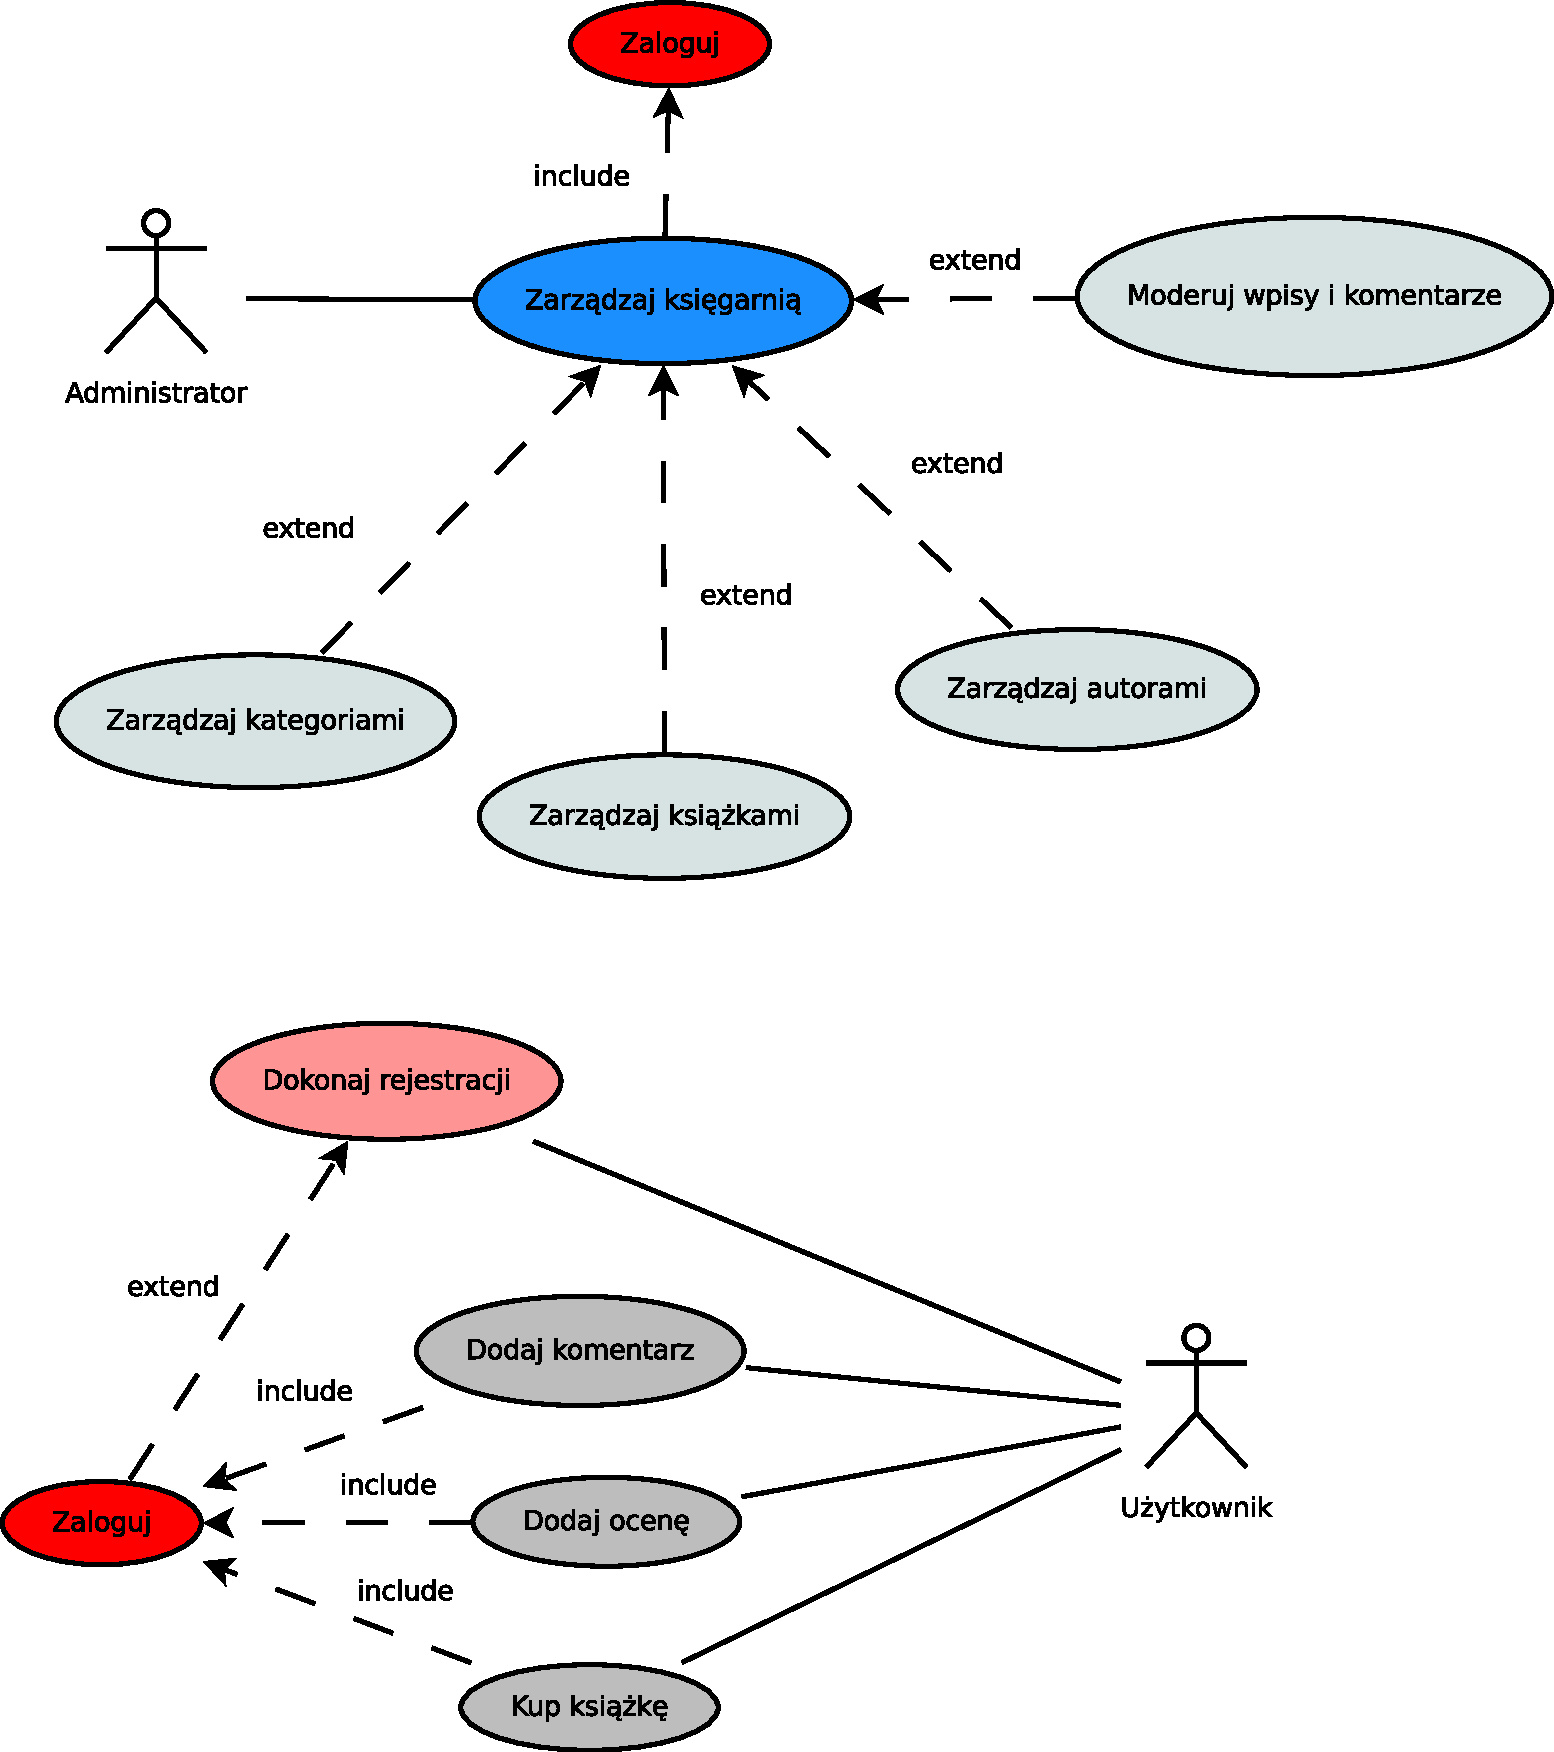
\includegraphics[scale=0.4]{usecase.pdf}
\label{fig:usecase}
\end{figure}


Aplikacja powinna w jak najwi�kszym stopniu odci��a� serwer WWW od niepotrzebnych zapyta�. W tym celu akcje usuwania, oceniania i komentowania ksi��ek b�d� realizowane przez kod JavaScript. Dodatkowo, cz�� walidacji danych b�dzie w pierwszej fazie wykonywana r�wnie� przy u�yciu \textit{front-endu}. Dopiero w wypadku wy��czenia wykonywania skrypt�w, wys�ane zostanie ��danie do sprawdzenia przez serwer. Takie podej�cie powinno znacznie zredukowa� obci��enie na przyk�ad podczas rejestracji u�ytkownik�w, poniewa� serwer wykonuje tylko minimum swojej pracy (\textit{Lazy Loading}).

Nale�y jednak mie� na uwadze bezpiecze�stwo oprogramowania, dlatego nie nale�y polega� w 100\% na walidacji wykonywanej przez JavaScript, poniewa� u�ytkownik mo�e bez problemu wy��czy� dzia�anie skrypt�w. Dlatego te� podczas tworzenia tego typu rozwi�za�, walidacja po stronie klienta powinna i�� zawsze w parze z walidacj� po stronie serwera.

Ze wzgl�du na konserwacj� i rozw�j tworzonej aplikacji, jest ona zarz�dzana przy pomocy systemu kontroli wersji \textit{git} w ramach serwisu \textit{http://github.com}. W ten spos�b tworzony kod jest pod �cis�� kontrol�, mo�e by� potem rozwijany przez wi�cej ni� jednego programisty, eliminuj�c konflikty podczas pracy na wsp�lnych zasobach.

Aplikacja wykorzystuje j�zyk HTML5, kt�ry staje si� powoli standardem tworzenia kodu po stronie klienta. Zawiera bowiem wiele nowoczesnych mechanizm�w i udogodnie� w stosunku do poprzedniej wersji na przyk�ad \textit{HTML4} oraz \textit{XHTML 1.0}. Maj�c na uwadze prawid�owe funkcjonowanie w poszczeg�lnych przegl�darkach i r�n� implementacj� nowego standardu, aplikacja wykorzystuje dodatek \texttt{HTML5} \texttt{Boilerplate} oraz 
\texttt{Twitter Bootstrap} jako metod� na otrzymanie podobnych rezultat�w w szerokiej gamie urz�dze� (w tym urz�dzenia mobilne). Jednocze�nie komponenty wchodz�ce w sk�ad \texttt{Twitter Bootstrap} umo�liwiaj� �atwe tworzenie komponent�w interfejsu u�ytkownika z ju� istniej�cych element�w.\\

Dost�p do danych w aplikacji mo�liwy jest dzi�ki \textit{webserwisom} udost�pniaj�cych pewien interfejs dost�powy. W ten spos�b szczeg�y implementacyjne s� ukryte, a u�ytkownik wykorzystuje tylko te funkcjonalno�ci, kt�re s� mu faktycznie potrzebne. W celu uproszczenia implementacji \textit{webserwis�w} wykorzystano rozszerzenie Piston dla frameworka \textit{Django}.

Projektowana aplikacja wykorzystuje technologi� AJAX (ang. \textit{Asynchronous
JavaScript and XML} - \textit{asynchroniczny JavaScript i XML} ), dzi�ki czemu mo�liwa jest symulacja zachowania aplikacji desktopowej. Reakcja na akcje u�ytkownika nast�puje bez potrzeby prze�adowania strony. Pozwala to na du�� oszcz�dno�� przepustowo�ci i czasu koniecznego do przetworzenia
ca�ej strony. Dzi�ki zastosowaniu frameworka \textit{jQuery} dla j�zyka JavaScript, mo�liwe jest stosowanie bardziej przyjaznego interfejsu u�ytkownika, przy jednoczesnym zapewnieniu kompatybilno�ci wstecz z istniej�cymi wersjami przegl�darek internetowych. Dzi�ki zaimplementowanym \textit{webserwisom}, zwracaj�cym dane w formacie \textit{JSON}, przetwarzanie i wy�wietlanie danych mo�e by� wykonane w�a�nie po stronie klienta z u�yciem \textit{JavaScript} i wbudowanych mechanizm�w przetwarzania ��da�.

\section{Budowa aplikacji}

Zaprojektowana aplikacja sk�ada si� tak naprawd� z dw�ch niezale�nych podaplikacji, jedna z nich hostowana jest wykorzystuj�c us�ug� \textit{Google Application Engine}, kt�ra zostanie om�wiona w rozdziale \ref{cha:architektura}. Aplikacja ta b�dzie udost�pnia�a us�ugi oparte o architektur� \textit{REST} (ang. \textit{Representation State Transfer}). B�dzie zawiera�a r�wnie� panel administracyjny do zarz�dzania ksi�garni�. Jest ona napisana w j�zyku \textit{Python}, wykorzystuj�c framework \textit{Django}, a tak�e wtyczk� \textit{Piston}, umo�liwiaj�c� proste wystawienie webserwis�w na podstawie modelu bazy danych.

Druga aplikacja b�dzie zawiera�a zakres funkcjonalny zwyk�ego u�ytkownika, natomiast wszystkie dane b�dzie pobiera�a przy u�yciu udost�pnionych przez wcze�niej omawian� aplikacje \textit{webserwis�w}. Aplikacja ta b�dzie napisana w j�zyku PHP z wykorzystaniem frameworka \textit{symfony}.\\

Obydwie aplikacje wykorzystuj� wzorzec MVC do separacji warstw logiki, prezentacji i danych. Dodatkowo, wykorzystane frameworki s� stworzone do szybkiego tworzenia oprogramowania, dzi�ki za�o�eniom \textit{scaffoldingu} oraz konwencjom \textit{DRY} (ang. \textit{Don't repeat Yourself}) i \textit{KISS} (ang. \textit{Keep it simple stupid}).

Schemat budowy aplikacji przedstawia rysunek \ref{fig:budowa_aplikacji}. 
Ka�dy element w systemie posiada szereg zale�no�ci, kt�rych nieprawid�owe dzia�anie poci�ga wiele daleko id�cych konsekwencji. Dlatego istotne jest, by kod aplikacji by� sp�jny i posiada� modularn� budow�. Umo�liwi to �atwiejsze wykrywanie problematycznych aspekt�w aplikacji, istotnych dla prawid�owego dzia�ania ca�ego projektu. 

\begin{figure}[htbp]
\center
\caption{Diagram budowy aplikacji ksi�garni internetowej}
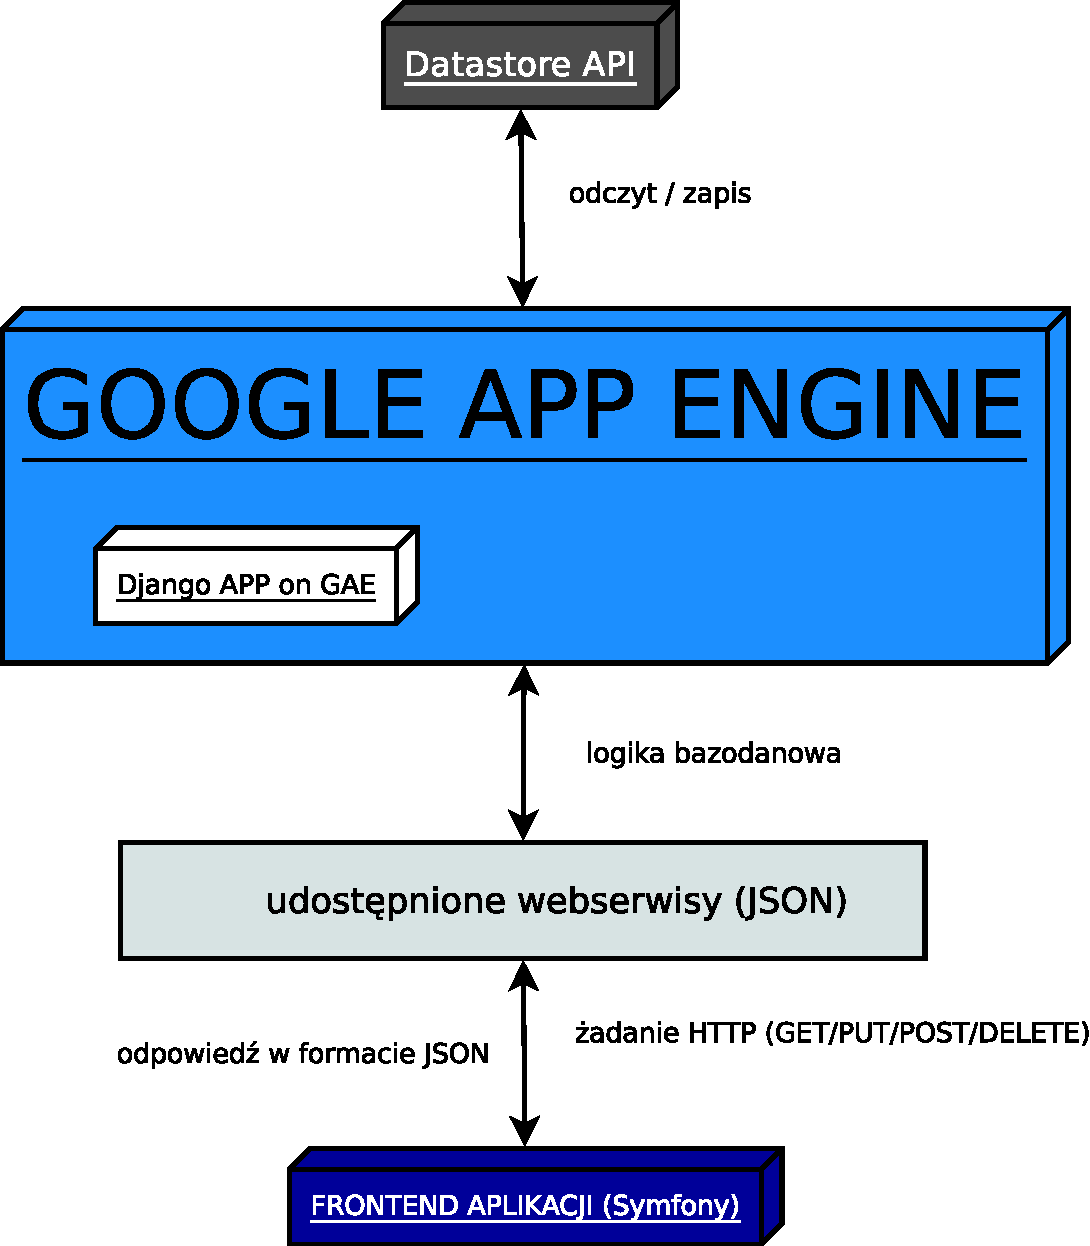
\includegraphics[scale=0.5]{diagram_aplikacji.pdf}
\label{fig:budowa_aplikacji}
\end{figure}


\section{Projekt bazy danych}

Rysunek \ref{fig:baza_danych} przedstawia projekt bazy danych wykorzystanej w ramach projektu. Diagram ERD przedstawia jednak baz� w podej�ciu relacyjnym, w p�niejszej cz�ci pracy pokazana zostanie baza NoSQL oraz proces de-normalizacji, kt�ry musia� zosta� dokonany. Na szcz�cie dzi�ki opisanemu w nast�pnym rozdziale frameworkowi \textit{Django-norel}, mo�liwe jest �atwe przechodzenie mi�dzy istniej�cymi implementacjami baz danych.

Baza zawiera ksi��ki, powi�zane z nimi s�owa kluczowe i kategorie. Ka�da ksi��ka ma swojego wydawc�. Dodatkowo, u�ytkownicy mog� komentowa� wybrane ksi��ki, ��cznie z wystawieniem oceny. Istotnym zamierzeniem projektowanego schematu by�a jak najwi�ksza optymalizacja u�ytych p�l. Na przyk�ad ocena w komentarzu ma warto�ci mi�dzy 1 a 5, wi�c wykorzystano typ danych \texttt{UNSIGNED INT(1) NOT NULL}, kt�ry przechowuje warto�ci od 0 do 255, bez sk�adowania warto�ci pustej. Do przechowywania has�a wykorzystano typ \texttt{CHAR(32)}, poniewa� w bazie przechowywana jest warto�� skr�tu has�a przy u�yciu algorytmu \textit{SHA1}.\\

Ze wzgl�du na pewne ograniczenia bazy \textit{Google Datastore}, konieczne by�o stworzenie pewnej nadmiarowo�ci w schemacie \texttt{book} oraz \texttt{category}. Poniewa� w \textit{GAE} nie funkcjonuj� \textit{z��czenia}, tabela \texttt{book} przechowuje list� identyfikator�w kategorii (\texttt{categories}) w celu imitacji zachowania dla relacji \textit{wiele do wielu}. Nale�y doda�, �e \textit{GAE}, posiada tym danych zdolny do przechowywania list wska�nik�w do poszczeg�lnych encji, jak r�wnie� liczb ca�kowitych i �a�cuch�w znakowych. Dodatkowo posiada metody do sprawdzania przynale�no�ci zadanych warto�ci do zbior�w opisanych przez te listy. Kolejnym elementem specyficznym dla tej platform s� pola zliczaj�ce - imituj�ce dzia�anie funkcji grupuj�cych. Pole \texttt{count} zawiera, wi�c informacj� o ilo�ci ksi��ek w danej kategorii. Podobne zastosowanie ma pole \texttt{average} tabeli \texttt{book}. Zawiera ono �redni� g�os�w wystawionych w komentarzach.

W celu osi�gni�cia zachowania funkcji grupuj�cych konieczne jest \textit{przeci��enie} metod zapisu dla obiekt�w reprezentuj�cych bazodanowe encje (Listing \ref{listing:model_overload}). 

\begin{lstlisting}[language=python, caption=Przeci��enie metody zapisu dla klas reprezentuj�cych encje \texttt{book} oraz \texttt{comment}, label=listing:model_overload]
class Comment(models.Model):
    
    def save(self, force_insert=False, force_update=False, using=None):
        
        comments = Comment.objects.filter(book = self.book)
        average = 0.00
         
        for comment in comments:
            average += comment.grade

        self.book.average = self.grade if not average else (average + float(self.grade)) / (comments.count() + 1)
        self.book.save()
        
        super(Comment, self).save()


class Book(models.Model):
    def save(self):
        
        if self.id is None:
            for category in self.categories:
                c = Category.objects.get(id = category)
                c.count = 1 if not c.count else c.count + 1
                c.save()
            
        super(Book, self).save()

\end{lstlisting}

Podczas projektowania nale�y mie� na uwadze specyfik� u�ycia poszczeg�lnych tabel. Dla tabel \texttt{kategorii} i \texttt{ksi��ek} dominowa� b�d� operacje odczytu, natomiast dla tabeli komentarzy operacje zapisu.

Poniewa� z za�o�enia dost�p do danych b�dzie realizowany poprzez udost�pnione us�ugi, rysunek \ref{fig:uslugi} przedstawia ich definicje, a tak�e metody komunikacji. W ten spos�b tylko za pomoc� odpowiednich metod HTTP (PUT - tworzenie, POST - tworzenie / aktualizacja, GET - pobieranie), mo�liwe jest wykonywanie odpowiedniej logiki.

\begin{figure}[htbp]
\caption{Us�ugi udost�pnione na platformie \textit{GAE} (\textit{Google Application Engine}) }
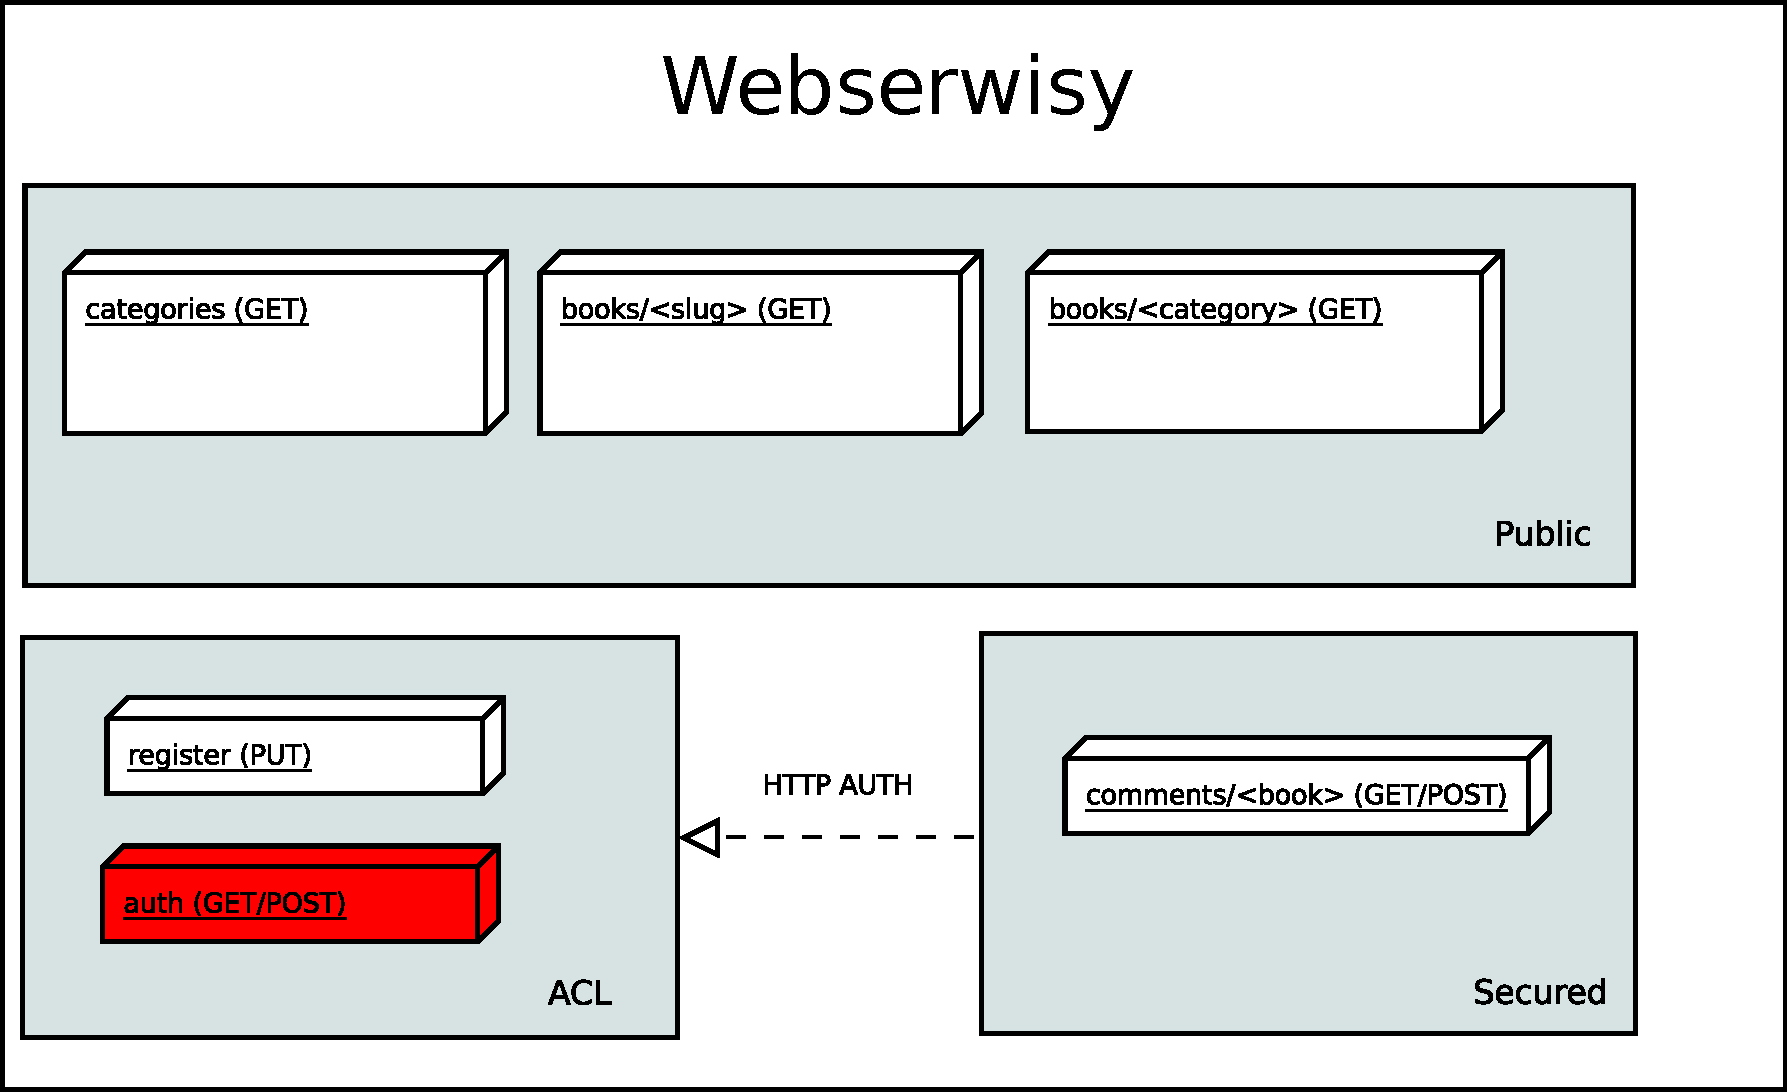
\includegraphics[scale=0.5]{serwice.pdf}
\label{fig:uslugi}
\end{figure}


\begin{sidewaysfigure}
\centering%
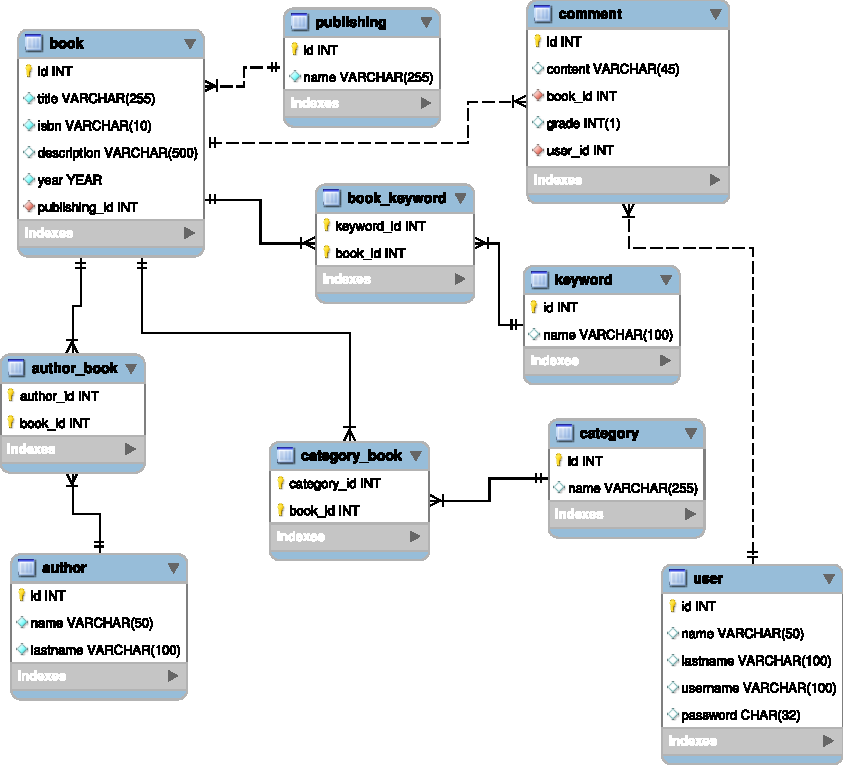
\includegraphics[scale=1]{db.pdf}
\caption{Projekt bazy danych aplikacji ksi�garni internetowej}
\label{fig:baza_danych}
\end{sidewaysfigure}
\chapter{Architektura aplikacji}
\label{cha:architektura}
Istotnym celem pracy jest zapewnienie mo�liwie najlepszej w danej chwili wydajno�ci. Twierdzenie to powinno by� prawdziwe r�wnie� w�wczas, kiedy aplikacja znajduje si� pod silnym ruchem sieciowym. Aby to zapewni�, konieczne jest wykorzystanie odpowiedniej architektury aplikacji.\\

Od kilku lat na rynku IT mo�na zaobserwowa� du�e zainteresowanie zwi�zane z chmurami obliczeniowymi (ang. \textit{Cloud Computing}). Jeszcze wi�ksze zamieszanie na rynku spowodowa�o udost�pnienie przez Google oraz Microsoft ich flagowych produkt�w znanych jako \textit{Google Application Engine} (GAE) oraz \textit{Windows Azure}. S� to us�ugi kwalifikowane jako \textit{PaaS}, czyli \textit{Platform as a Service}. Oznacza to, �e korzystaj�c z ich produkt�w otrzymujemy kompletne �rodowisko uruchomieniowe aplikacji oraz zaplecze technologiczne umo�liwiaj�ce uruchamianie aplikacji. W wypadku GAE mo�liwe jest programowanie aplikacji z wykorzystaniem udost�pnionego przez us�ug� zbioru bibliotek, napisanych w trzech j�zykach: Java, Python oraz Go. Nast�pnie przy pomocy udost�pnionych narz�dzi mo�liwe jest wdro�enie aplikacji (\textit{Deployment}).\\

Takie podej�cie do tworzenia aplikacji internetowych zyska�o olbrzymi� ilo�� zwolennik�w, poniewa� pozwoli�o na ca�kowite przeniesienie ci�aru zarz�dzania skomplikowan� infrastruktur� na producent�w rozwi�za� \textit{Paas}. Innym wa�nym powodem, dla kt�rego wielu ludzi zdecydowa�o si� na wykorzystanie nowych us�ug, jest mo�liwo�� konfiguracji architektury do w�asnych potrzeb, a tak�e (co by�o kluczowym powodem), do aktualnego obci��enia aplikacji.

Preferowanie \textit{cloud computingu} jest nap�dzanie przez wiele czynnik�w, w�r�d kt�rych nale�y wymieni� �atwo�� dost�pu - wszystko czego potrzeba to przegl�darka. Z drugiej strony r�wnie wa�na jest �atwo�� zarz�dzania - nie potrzeba etatu do do�wiadczonego administratora. Mo�liwo�ci chmur obliczeniowych s� docenianie tak�e przez dostawc�w us�ug ze wzgl�du na �atwe zarz�dzanie infrastruktur�, poniewa� centra danych posiadaj� jednorodny sprz�t i oprogramowanie, co wi�cej s� one pod kontrol� jednego kompetentnego podmiotu \cite{book:cloud2}.

\section{Rodzaje chmur}
\label{sec:rodzaje_chmur}

\begin{figure}[H]
\caption{Zestawienie rodzaj�w chmury ze wzgl�du na udost�pniane zasoby}
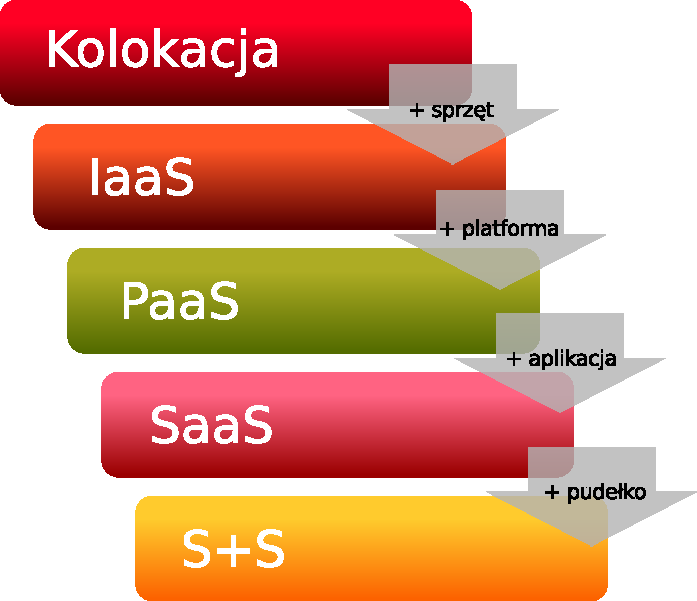
\includegraphics[scale=0.75]{chmura_model.pdf}
\label{fig:chmury}
\end{figure}

Najog�lniej chmury dziel� si� na \textit{prywatne} i \textit{publiczne}. Prywatne wchodz� w sk�ad cz�ci organizacji, ale jednoczesne stanowi� autonomiczn� us�ug�. Publiczne natomiast udost�pniane s� przez zewn�trznych dostawc�w us�ug \cite{book:cloud}.

Rysunek \ref{fig:chmury} pokazuje zasadnicze r�nice mi�dzy poszczeg�lnymi rodzajami chmur. Chmura oferowana przez \textit{Google Application Engine}, zapewnia wsparcie w zakresie architektury serwera, systemu plik�w, a tak�e systemu bazodanowego. Dodatkowo, \textit{GAE} udost�pnia r�wnie� mo�liwo�� korzystania z us�ug w tle oraz serwer�w mailowych, a tak�e wiele mniejszych us�ug takich jak wykonywanie ��da� do zewn�trznych us�ug. Nowo�ci� w fazie test�w jest tak�e mo�liwo��, rozdzielenie obci��enia na kilka wersji aplikacji (\textit{traffic splitting}).\\

Najprostszym i najstarszym rodzajem us�ug w "chmurze" jest \textit{Kolokacja}. Polega ona na dzier�awieniu miejsca w serwerowni, pr�du, klimatyzacji i po��czenia do Internetu. W gestii dzier�awcy jest zaopatrzenie si� w sprz�t, zabezpieczenia, system operacyjny ko�cz�c na oprogramowaniu i aplikacjach.

Bardziej rozbudowanym rodzajem chmury jest \textit{IaaS} (ang. Infrastructure as a Service), czyli rozszerzenie kolokacji o zapewnienie sprz�tu przez dostawc�. To dostawca udost�pnia sprz�t, niejednokrotnie r�wnie� zabezpieczenia. Zadaniem odbiorcy jest dostarczenie systemu operacyjnego, oprogramowania i aplikacji. Pewn� grup� us�ug, kwalifikowan� do tego zbioru, mog� by� serwery dedykowane, kt�re u wielu dostawc�w mo�na kupi� od dawna. Obecnie jednak zakres mo�liwo�ci serwer�w dedykowanych zosta� poszerzony, dzi�ki wykorzystaniu technologii wirtualizacji. Za jej spraw�, u�ytkownik otrzymuje funkcjonaln� maszyn� wirtualn�, kt�r� mo�e skonfigurowa� w dowolny spos�b wykorzystuj�c zdalny dost�p.

Jak wynika z zestawienia rodzaj�w chmur, us�uga \textit{PaaS}, a wraz z ni� r�wnie� \textit{GAE} oferuje du�o wi�cej ponad standardow� infrastruktur� sprz�tow�. U�ytkownik musi si� skupi� jedynie na dostarczeniu oprogramowania pracuj�cego w okre�lonym �rodowisku roboczym.

Polityk� chmur typu \textit{PaaS} jest p�acenie tylko za aktualne zu�ycie
zasob�w. Rozliczani jeste�my wiec, za moc obliczeniow� serwer�w i czas ich pracy, ilo�� zapyta� do bazy, a tak�e za bie��ce wykorzystanie dysku. Dodatkowo architektura dynamicznie zwi�ksza ilo�� zasob�w, jak r�wnie� instancji serwer�w aktualnie
wykorzystywanych, by jak najbardziej zmniejszy� czas odpowiedzi
strony (Rys. \ref{fig:komponentyCloud}). Ca�o�� mo�na dynamicznie kontrolowa� balansuj�c koszty do optymalnej szybko�ci dzia�ania aplikacji.

\begin{figure}[htbp]
\caption{Komponenty wchodz�ce w sk�ad architektury w chmurze}
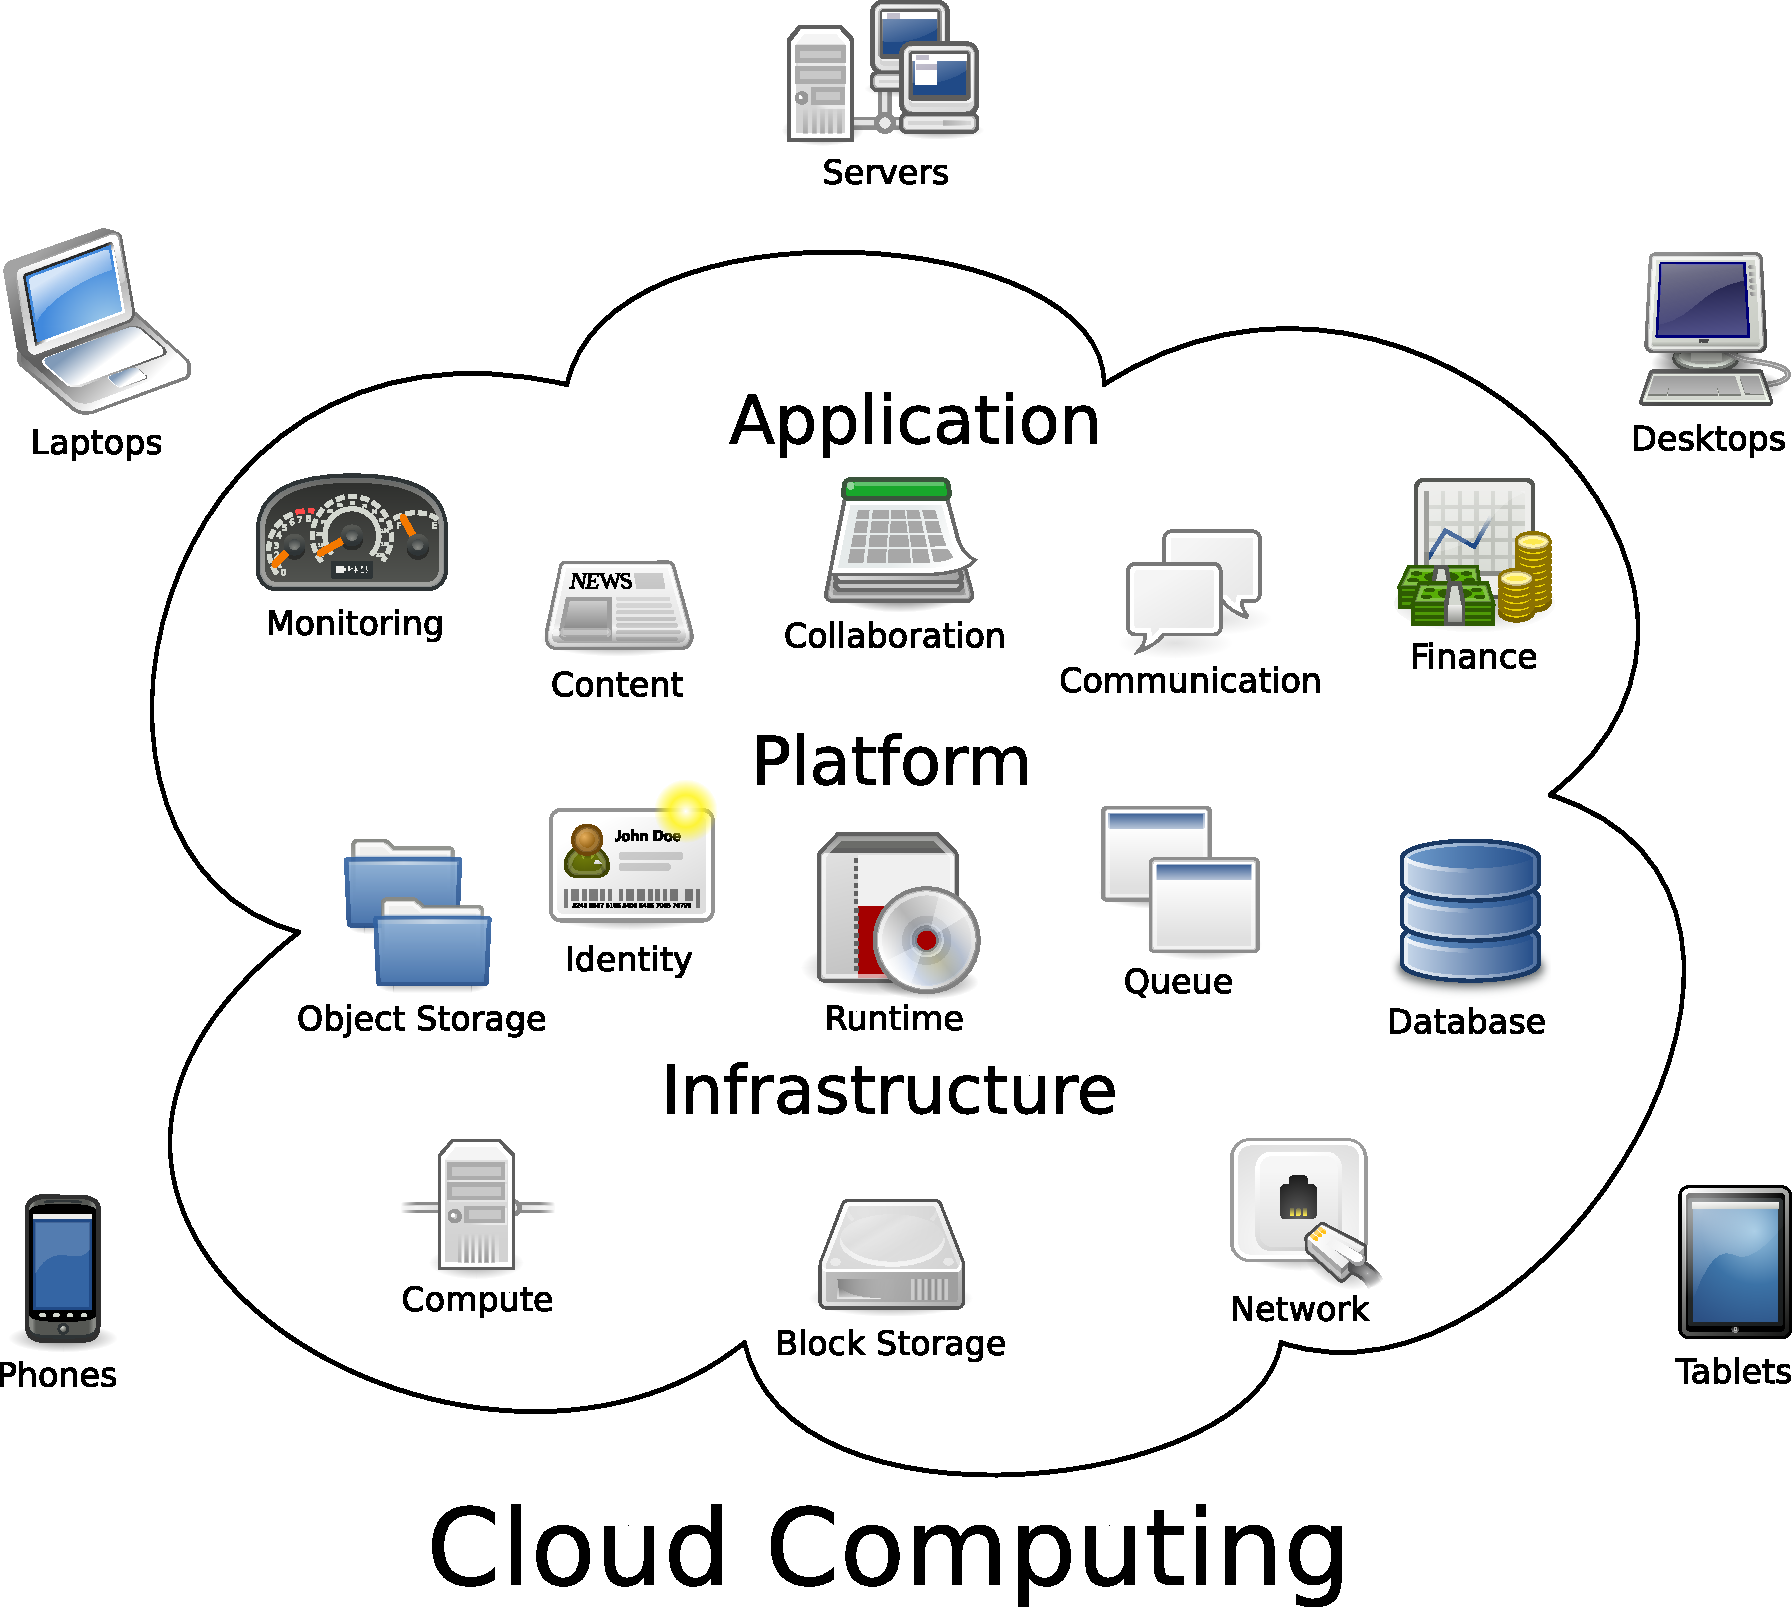
\includegraphics[scale=0.4]{Cloud_computing.pdf}
\label{fig:komponentyCloud}
\end{figure}


W wypadku GAE w ramach darmowych limit�w do dyspozycji dostajemy 28h instancji. Oznacza to, �e w wypadku pojedynczej najwolniejszej instancji b�dziemy mogli z niej korzysta� 28h (600Mhz), w wypadku szybszej instancji (1200Mhz) czas ten zostanie 2-krotnie zmniejszony. W wypadku najszybszej instancji (2400Mhz) czas ten ulega 4-krotnemu skr�ceniu. Do oceny u�ytkownika zostaje decyzja, z jakiej instancji chce korzysta� i oczywi�cie, jak bardzo ilo�� serwer�w b�dzie si� zwi�ksza�a przy nat�eniu ruchu. Je�li darmowa oferta GAE jest niewystarczaj�ca, w ka�dej chwili mo�na przej�� na opcj� p�atn�, w kt�rej okre�lamy tygodniowe / miesi�czne limity p�atno�ci. Jedn� z wa�nych zmian w por�wnaniu z normalnymi hostingami jest taryfikator operacji bazodanowych. Wyr�niono ceny za odczyt i zapis do bazy, odpowiednio 0.10\$ za 100,0000 operacji zapisu i 0.07\$ za podobn� ilo�� operacji odczytu. System liczenia operacji zapisu opera si� na dodatkowych operacjach, zwi�zanych z indeksowaniem danych. Przyk�adowo pobranie pojedynczego rekordu z bazy to koszt jednego odczytu, ale wykonanie zapytania zwracaj�cego 20 rezultat�w to koszt 21 operacji odczytu. W wypadku zapisu do bazy nowej encji oznacza to 2 operacji zapisu + 2 operacje zapisu na ka�dy indeks dla pola + 1 zapis dla warto�ci indeksu z�o�onego.

Rysunek \ref{fig:gae_dashboard} przedstawia pogl�dowy widok bie��cych statystyk aplikacji, udost�pnianych przez GAE. U�ytkownik ma dost�p do stan�w bie��cych limit�w, a tak�e szczeg�owych wykres�w wydajno�ci aplikacji okre�lanych na podstawie r�nych czynnik�w (zaj�to�� pami�ci, ilo�� operacji na sekund�, wykorzystanie instancji serwer�w). Bardzo przydatny jest r�wnie� wykres bie��cej aktywno�ci aplikacji. W ten spos�b mo�na szybko oceni�, czy aplikacja jest obecnie pod du�ym obci��eniem, a tak�e por�wna�, czy na przyk�ad wdro�one zmiany poprawi�y jej wydajno��.

\begin{figure}[htbp]
\caption{Wygl�d panelu statystyk w ramach us�ugi \textit{GAE}}
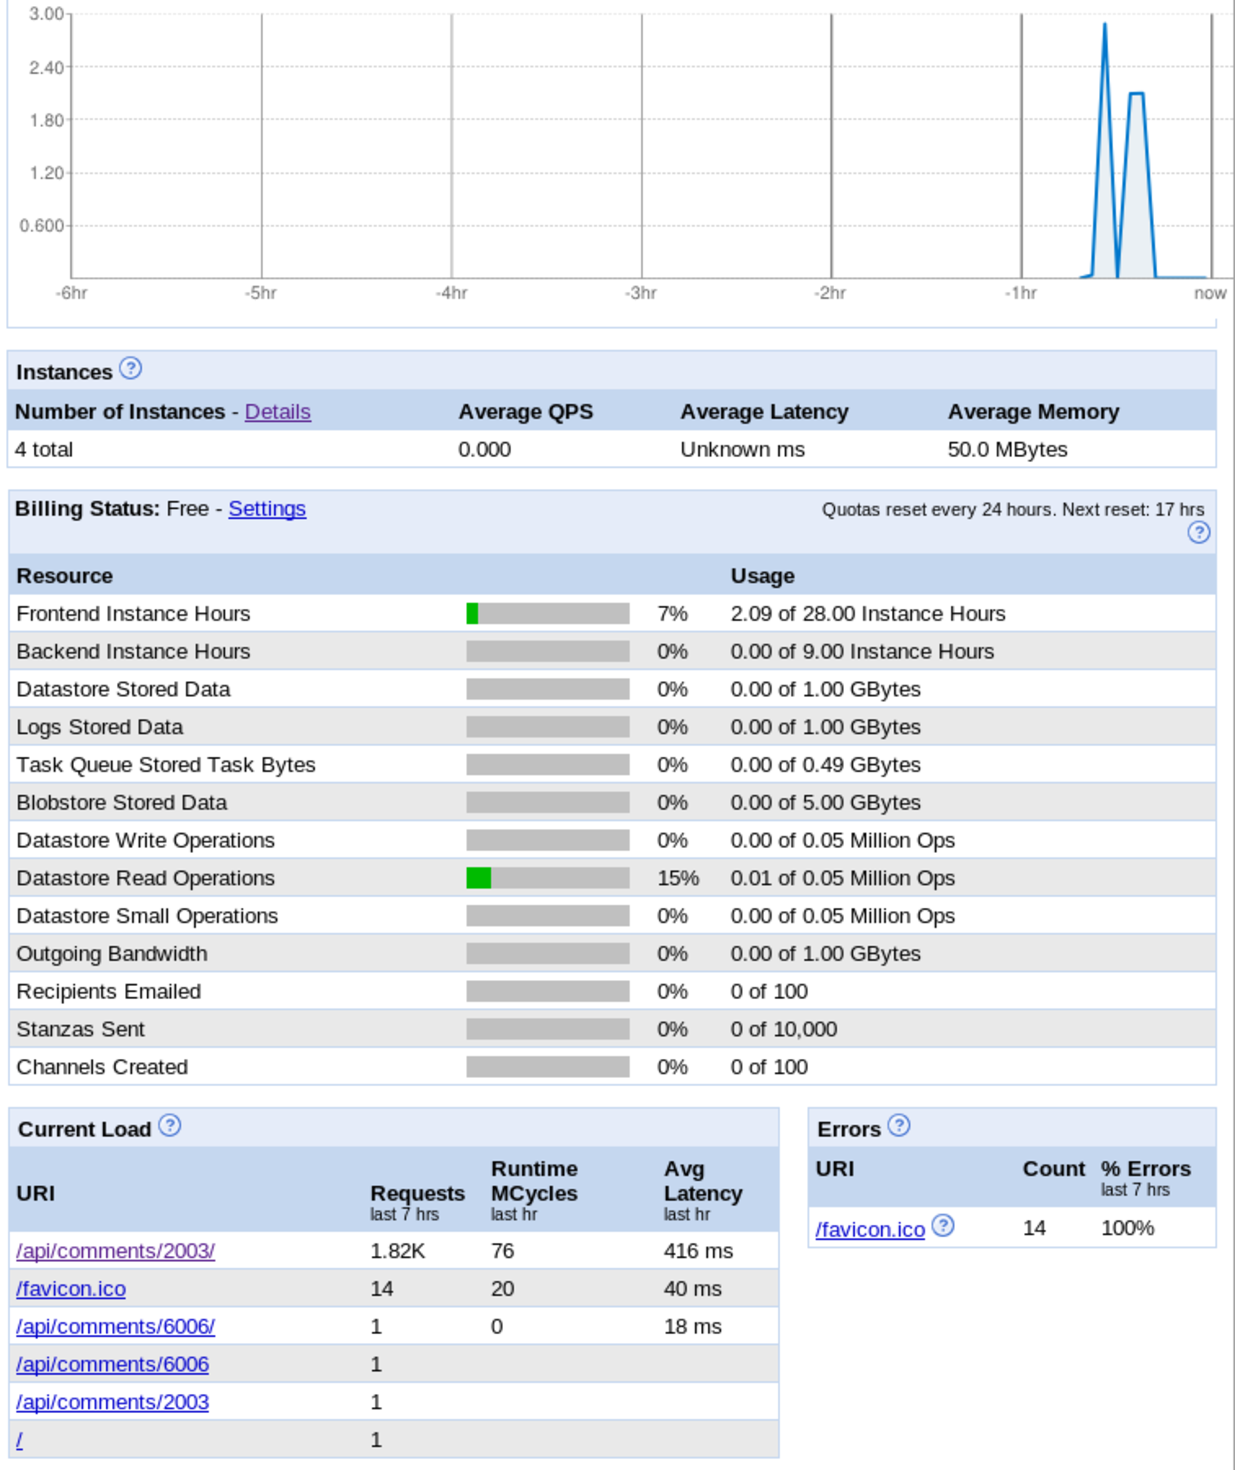
\includegraphics[scale=0.7]{gae_dashboard.pdf}
\label{fig:gae_dashboard}
\end{figure}

\section{Zarz�dzanie wydajno�ci� aplikacji na platformie \textit{GAE}}

Jak zosta�o om�wione we wst�pie w podrozdziale \ref{sec:rodzaje_chmur},  olbrzymi� zalet� rozwi�za� \textit{PaaS} jest mo�liwo�� kompleksowego zarz�dzania aplikacj� z poziomu przegl�darki i udost�pnionego interfejsu klienta. Rysunek \ref{fig:performance} pokazuje jak to wygl�da w praktyce. Za pomoc� listy dost�pnej w sekcji \textit{Frontend Instance Class} okre�lamy jak bardzo wydajnej instancji chcemy u�y� dla naszej aplikacji. Ka�da z instancji jest opisana za pomoc� umownego symbolu, cz�stotliwo�ci pracy procesora oraz maksymalnej dost�pnej pami�ci. Przy obecnym ustawieniu ka�da utworzona instancja serwera posiada� b�dzie parametry instancji \textit{F1}.

W celu zapewnienia wydajno�ci aplikacji na okre�lonym poziomie, wa�ne jest wywa�enie ustawie� dw�ch suwak�w, odpowiednio \textit{Max Idle Instances} oraz \textit{Min Pending Latency}. Pierwszy suwak okre�la pocz�tkow� ilo�� instancji dost�pn� zawsze (tak zwani \textit{rezydenci}). W wypadku kolejnych instancji, ich ilo�� jest warunkowana parametrami okre�lonymi przez  punkty brzegowe drugiego suwaka. Okre�la on jak d�ugo \textit{dyspozytor} ��da� poczeka, nim zadecyduje o odes�aniu ��dania do innej instancji serwera. Jest to bardzo logiczne za�o�enie, �e je�li ��danie wykonuje si� d�ugo, prawdopodobnie strona jest obci��ona, dlatego trzeba odci��y� serwery i roz�o�y� ruch na nowo dodane. 

\begin{figure}[htbp]
\caption{Kontrola wydajno�ci aplikacji w  \textit{GAE}}
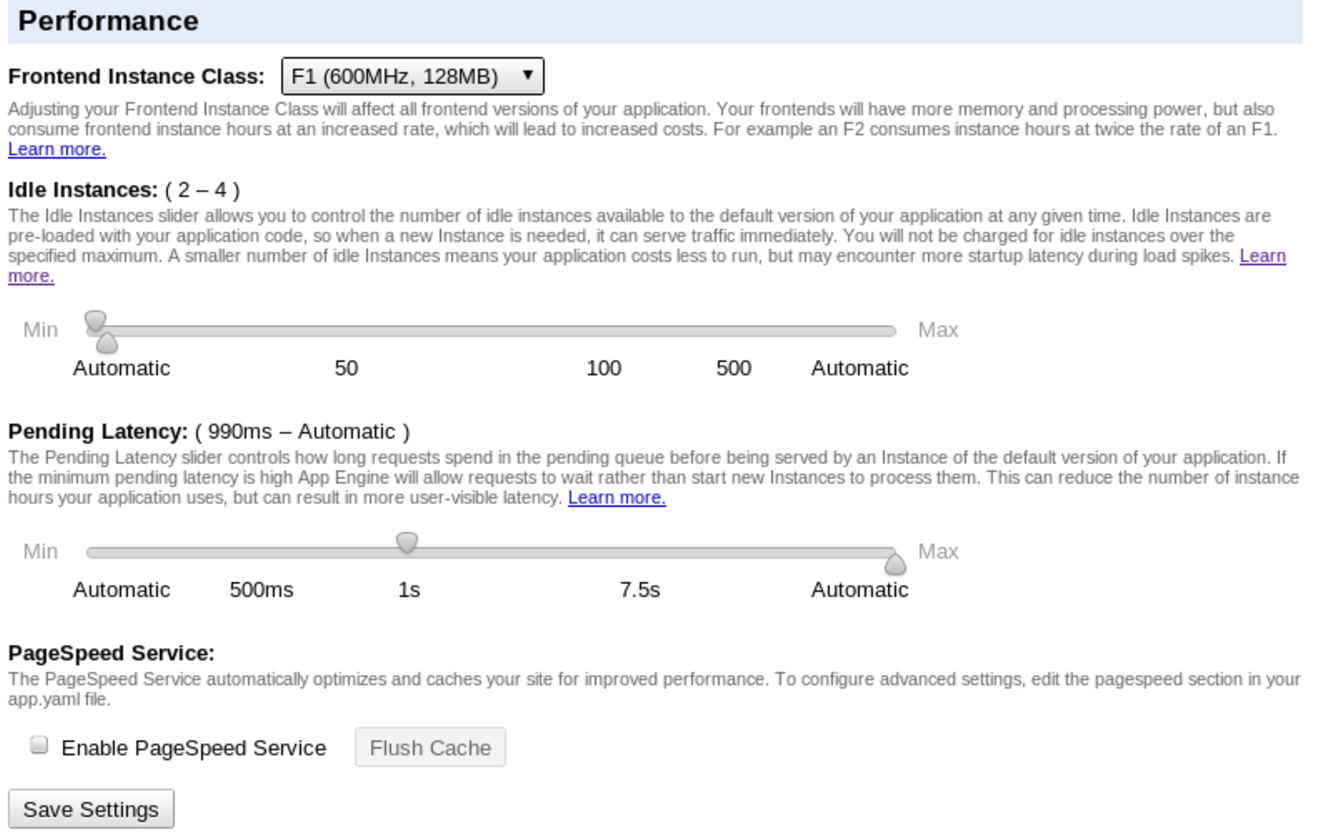
\includegraphics[scale=0.6]{performance.pdf}
\label{fig:performance}
\end{figure}

Je�li skonfigurowano serwer zgodnie z rysunkiem \ref{fig:performance}, w zak�adce \textit{Instances} powinny zosta� wy�wietlone wszystkie aktualnie wykorzystywane instancje serwer�w. Dwie z nich to instancje sta�e - rezydencji, wi�c ich czas pracy jest r�wny dobie. Dodatkowo widoczne s� r�wnie� instancje dynamiczne (Rys. \ref{fig:performance2}), czyli takie, kt�re u�ywane s� dora�nie. Zgodnie z ustawieniami, ��czna ilo�� instancji nie przekroczy g�rnego maksimum czyli czterech serwer�w. W wypadki instancji dynamicznych nale�y mie� na uwadze, �e na op�at� sk�ada si� sumaryczny czas pracy oraz 15-minutowy czas op�aty rozruchowej. Dla przyk�adu je�li dynamiczna instancja pracuje przez pi�� minut to koszt wynosi $0.08 / 60 \times  (15 + 5) = 2.6\cent$.

\begin{figure}[htbp]
\caption{Nadz�r i zarz�dzanie instancjami serwer�w w \textit{GAE}}
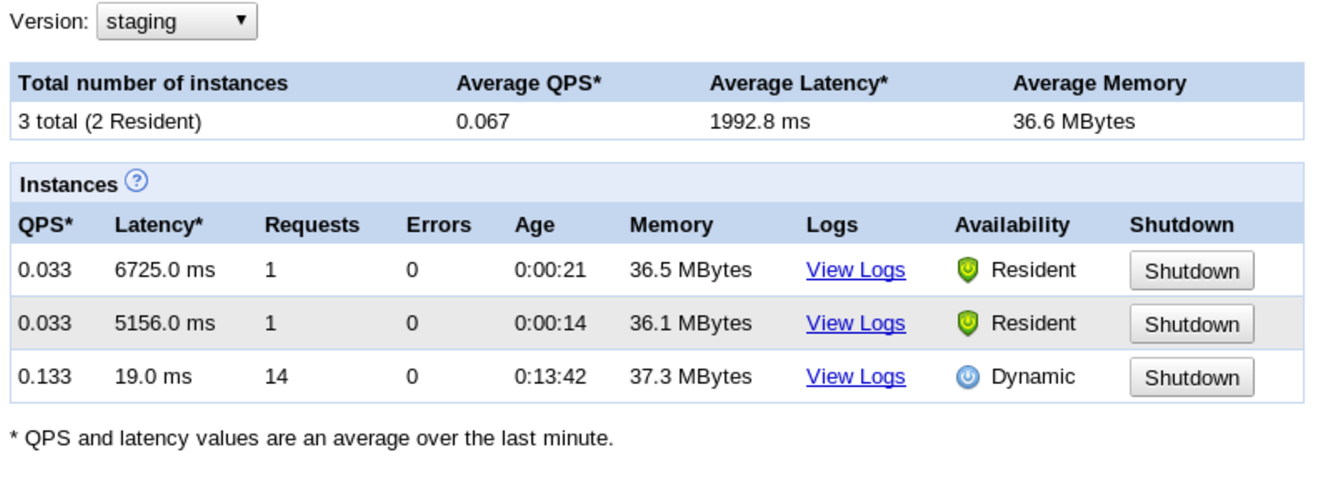
\includegraphics[scale=0.62]{performance2.pdf}
\label{fig:performance2}
\end{figure}

W zak�adce \textit{Instances} mo�na r�wnie� zobaczy� takie statystyki jak ilo�� operacji na minut� (\textit{Average QPS}), �rednie zu�ycie pami�ci (\textit{Average Memory}) czy �redni czas przetwarzania ��dania (\textit{Average Latency}). Dodatkowo je�li kt�ra� z instancji uleg�a przeci��eniu, w skutek czego nie reaguje, mo�na j� zamkn�� r�cznie, klikaj�c przycisk \textit{Shutdown}.

\section{Nierelacyjne bazy danych \textit{NoSQL}}

Od pocz�tku ery informatyzacji, informacja i jej przechowywanie by�o najwa�niejszym zadaniem powierzanym komputerom. Bazy danych musz� zar�wno przechowywa� dane (zapis), jak i udost�pnia� interfejs s�u��cy ich odczytowi, a nawet wyszukiwaniu w oparci o zadane kryteria. Dotychczas wykorzystywano g��wnie relacyjne bazy danych, kt�re ��czy�y pojedyncze tabele w r�nego rodzaju asocjacje. Wcze�niej jednak konieczne jest zdefiniowanie okre�lonego schematu bazy danych, kt�ry b�dzie obowi�zywa� i nak�ada� ograniczenia na dane.

Obecnie jednak bardzo popularne staj� si� bazy bez okre�lonej
struktury, niesamowicie skalowalne, a przy tym dost�p do niech
odbywa si� przy pomocy \textit{REST}owego API.
Wyr�niono kilka konwencji:
\begin{itemize}
\item{\textit{Key Value Stores} - HDOOP, BigData},
\item{\textit{Graph Databases} - Neo�tj, AllegroGraph},
\item{\textit{BigTables} - HBase, Cassandra},
\item{\textit{Document Database} - MongoDB, CoachDB, SimpleDB}
\end{itemize}

W projektach \textit{e-commerce} najwi�kszym zastosowaniem ciesz� si�
bazy dokumentowe, skupiaj�ce kolekcje obiekt�w - dokument�w.
Ka�dy z nich mo�e zawiera� odpowiednie metadane i s�owa
kluczowe. Ka�dy dokument posiada dowoln� definicj� i mo�e by�
dowolnie zagnie�d�any i ��czony z innymi dokumentami.\\

Wraz z wykorzystaniem nie-relacyjnych baz danych, zmieni� si� zupe�nie pomys� na organizacj� danych. Si�� baz danych NoSQL jest brak �ci�le okre�lonej struktury, przez co schemat danych mo�e si� dowolnie zmienia� w trakcie rozwoju aplikacji. Innym wa�nym powodem wykorzystania bazy \textit{Google Datastore}, oferowanej przez GAE jest szybko�� i skalowalno��. W odr�nieniu od zwyk�ego hostingu, baza danych w GAE mo�e by� rozproszona na dowoln� ilo�� instancji.\\

Pocz�tkowo osoby korzystaj�ce z baz nierelacyjnych zarzuca�y takiemu rozwi�zaniu nast�puj�ce wady:

\begin{itemize}
\item{problem z ponownym wykorzystaniem kodu dla innych rozwi�za� nie relacyjnym nawet kiedy implementacje s� podobne,}
\item{nie mo�na wykorzysta� kodu dla relacyjnej bazy danych, nawet je�li schemat pozosta�by nietkni�ty,}
\item{konieczno�� zarz�dzania indeksami, a tak�e problem denormalizacji,}

\item{konieczno�� samodzielnej implementacji ��czenia rezultat�w wielu zapyta�,}

\item{niekt�re z rozwi�za� s� zintegrowane ze specyficznym dostawc� (\textit{App Engine}, \textit{SimpleDB}), wi�c u�ytkownik nie ma mo�liwo�ci migracji na inn� platform� bez du�ego nak�adu pracy.}
\end{itemize}

W stworzonej aplikacji wykorzystano framework \textit{Django-nonrel} dodaj�cy obs�ug� baz NoSQL do frameworka \textit{Django}. W ten spos�b mo�liwe jest wykorzystanie abstrakcji bazodanowej i tworzenie rozwi�za� niezale�nie od technologii bazy. Wszystko to mo�liwe jest dzi�ki wbudowanemu narz�dziu \textit{ORM} (ang. \textit{Object-Relational Mapping}), kt�re udost�pnia obiektowy interfejs dost�pu do danych. W ten spos�b pisana logika nie jest zale�na od konkretnej platformy lub rozwi�zania sk�aduj�cego.\\

\subsection{Specyfika \textit{Google Datastore}}

\textit{Google App Engine} posiada swoj� wewn�trzn� baz� danych \textit{Datastore}, kt�ra przechowuje obiekty danych, znane jako \textit{encje}. Ka�da encja ma jedn� lub wi�cej p�l r�nego typu podobnie, jak w relacyjnych bazach. Ka�da encja jest identyfikowana po jej typie, ma to na celu katalogowanie ich z wzgl�du na pe�nion� funkcj� logiczn�. Jest to pewna analogia do tabel, ale raczej nale�y to postrzega� jako kontenery na lu�no powi�zane obiekty. Ka�da encja ma klucz, kt�ry unikalne identyfikuje zas�b niezale�nie od typu \cite{book:gae}.\\

\textit{Datastore} mo�e wykonywa� wiele operacji w pojedynczej transakcji. Z za�o�enia transakcja nie mo�e si� zako�czy� do czasu zako�czenia ostatniej operacji w jej ramach. Oczywi�cie w wypadku niepowodzenia transakcja zosta�aby wycofana, co jest szczeg�lnie przydatne w wypadku rozproszonych aplikacji webowych, gdzie wielu u�ytkownik�w mo�e mie� dost�p lub wykonywa� operacje na tym samym obiekcie.

W GAE g��wnym miejscem sk�adowania jest HRD (\textit{High Replication Datastore}). W skr�cie, jest to miejsce, gdzie dane s� replikowane do wielu centr�w danych wykorzystuj�c system oparty na algorytmie \textit{Paxos}. Taki zabieg zapewnia wysoki poziom dost�pno�ci dla operacji odczytu i zapisu. Jedyny problem mo�e wyst�powa� ze sp�jno�ci� danych ze wzgl�du na czas replikacji do poszczeg�lnych w�z��w.\\

W odr�nieniu od standardowych baz danych, GAE wykorzystuje architektur� rozproszon�, aby zapewni� automatyczne zarz�dzanie skalowaniem nawet w wypadku bardzo obszernych zbior�w danych. Pomimo podobie�stw w mechanizmach dost�pu do danych mi�dzy poszczeg�lnymi bazami, istotn� r�nic� jest spos�b opisywania relacji pomi�dzy obiektami. Na przyk�ad encje tego samego typu mog� mie� r�ne pola, z kolei r�ne encje mog� mie� w�a�ciwo�ci tej samej nazwy, ale przechowywa� warto�ci r�nego typu. Te unikalne cechy sprawiaj�, �e projektowanie i zarz�dzanie danymi r�ni si� znacz�co w wypadku tej platformy. Poniewa� GAE jest stworzone do skalowania, w wypadku wzmo�onego zapisu, \textit{Datastore} automatycznie rozproszy dane, je�li jest to konieczne na wi�cej instancji. R�wnie� operacje odczytu s� dostosowane do szybkiego dzia�ania, poniewa� jedyne dozwolone zapytania to takie, kt�re dzia�aj� niezale�nie od wielko�ci danych.

Oznacza to, �e wyszukiwanie w zbiorze 100 elementowym zajmie dok�adnie tyle samo czasu, co w zbiorze zawieraj�cym ich milion. \textit{Datastore} robi r�wnie� du�y u�ytek z indeks�w dla kolekcji danych. Istotn� cech� jest fakt, �e w procesie tworzenia aplikacji, biblioteka deweloperska bada, kt�re zapytania wymagaj� dodania nowych indeks�w i robi to za u�ytkownika w specjalnym pliku definicji indeks�w. W ten spos�b najwa�niejsze zapytania wykonywane przez aplikacj� posiadaj� dane uporz�dkowane w odpowiednich indeksach. Je�li w aplikacji wykonywane s� operacje sortowania danych po jakiej� kolumnie to w GAE wyniki sortowania rosn�cego i malej�cego b�d� przechowywane w zupe�nie r�nych indeksach, nawet je�li dotycz� tego samego pola. 

\section{Aplikacja zorientowana na us�ugi}

Inn� wa�n� cech� tworzonej aplikacji jest wyszczeg�lnienie us�ug (\textit{webservice�w}), kt�re pomog� w wykonywaniu operacji na modelu przy pomocy metod protoko�u HTTP. B�d� to wi�c popularne w dzisiejszych czasach us�ugi REST. Ze wzgl�du na specyfik� aplikacji i du�y udzia� j�zyka JavaScript w tworzonej logice, w wi�kszo�ci wypadk�w us�ugi te b�d� zwraca�y dane w notacji \textit{JSON}.\\

Zalet� takiego podej�cia, okre�lanego p�niej jako \textit{Service Oriented Architecture} jest wydzielenie pewnych us�ug, zawieraj�cych pewn� cz�� / zakres funkcjonalny. W ten spos�b aplikacja jest podzielona na grup� takich us�ug, z kt�rych ka�da realizuje tylko i wy��cznie swoje zadanie. Dzi�ki takiej dekompozycji, mo�liwym staje si� wykorzystanie wspomnianych us�ug, wsz�dzie tam gdzie jest to potrzebne. Inn� zalet� jest �atwo�� testowania takich us�ug, poniewa� nie jest konieczne stworzenie ca�ego zestawu wykonawczego, a jedynie test konkretnego dzia�ania, spe�niaj�cego okre�lone cele.

Poniewa� komunikacja mi�dzy \textit{front-endem} aplikacji, napisanym w j�zyku \textit{PHP}, a zapleczem umiejscowionym na platformie GAE odbywa si� poprzez webserwisy, istotne by�o wyr�nienie nast�puj�cych us�ug:

\begin{itemize}
\item{us�uga zwracaj�ca dost�pne kategorie, a tak�e kategorie dla danej podkategorii,}
\item{us�uga wy�wietlaj�ca ksi��ki z danej kategorii,}
\item{us�uga wy�wietlaj�ca komentarze do danej ksi��ki,}
\item{us�uga dodaj�ca komentarz z ocen� do ksi��ki,}
\item{us�uga wyszukuj�ca ksi��ki na podstawie s��w kluczowych, tytu�u lub kategorii}
\end{itemize}

Ka�da us�uga zwraca obiekt \textit{JSON}, kt�ry nast�pnie jest analizowany przez kod \textit{JavaScript}. Takie podej�cie czyni przetwarzanie strony niezwykle wydajnym, bo obci��enie jest dzielone na dwie aplikacje.

\subsection{AJAX, a restrykcje bezpiecze�stwa kodu \textit{JavaScript}}

Na pocz�tku projektowania zaistnia� jeden problem wynikaj�cy z komunikacji przy u�yciu technologii AJAX. Problem \textit{same origin policy} jest bardzo istotnym za�o�eniem bezpiecze�stwa dotycz�cym j�zyk�w interpretowanych po stronie przegl�darki, takich jak \textit{JavaScript}. Polityka bezpiecze�stwa zezwala skryptom uruchamianym w ramach tej samej strony na dost�p do metod i w�a�ciwo�ci powi�zanych obiekt�w \textit{JavaScript} bez specjalnych restrykcji. Z drugiej strony polityka ta odmawia dost�pu do wi�kszo�ci metod i w�asno�ci podczas takich pr�b na innych stronach (inna domena, subdomena).

Mechanizm ten odciska znacz�ce pi�tno na nowoczesnych aplikacjach internetowych, kt�re w znacznym stopniu polegaj� na przyk�ad na danych uwierzytelniaj�cych, zapisanych w sesji \textit{HTTP cookie}, jak r�wnie� wykorzystuj�cych technologi� AJAX do pobierania rezultat�w dzia�ania us�ug.

\subsubsection{\textit{JSONP} (\textit{JSON with padding})}

JSONP stanowi dope�nienie bazowego formatu danych \textit{JSON}. Jest sposobem na obej�cie problemu dost�pu do danych z r�nych domen zwi�zanych z \textit{same origin policy}. Zgodnie z zasad�, strona umieszcona pod adresem \texttt{server1.example.com} nie mo�e normalnie po��czy� si� lub komunikowa� z serwerem innym ni� \texttt{server1.example.com}. Jedynym wyj�tkiem od tej regu�y jest HTML-owy element \texttt{<script>}. 

Obchodz�c regu�� bezpiecze�stwa, mo�liwe jest pobranie zwracanego kodu \textit{JavaScript}, kt�ry operuje na dynamicznie wygenerowanych danych w formacie \textit{JSON}. Tak naprawd� takie ��danie nie zwraca wcale obiektu \textit{JSON}, tylko dynamicznie utworzony kod \textit{JavaScript} i odnosi si� do metod istniej�cych na stronie wykonuj�cej ��danie.\\

Przyk�adowy kod obrazuj�cy ten spos�b widoczny jest na listingach \ref{listing:jsonp} oraz \ref{listing:jsonpserver}. Pierwszy skrypt pokazuje \textit{front-endow�} cz�� rozwi�zania, drugi natomiast zwraca kod \textit{JavaScript}, kt�ry wykona metod� \texttt{parseJSON} z przetworzonym obiektem \textit{JSON}, zawieraj�cym wynik dzia�ania zapytania bazodanowego jako parametr funkcji. Nast�pnie metoda \texttt{parseJSON} iteruj�c w p�tli po elementach obiektu JSON (w j�zyku \textit{JavaScript} obiekty s� r�wnie� tablicami, wi�c mo�na stosowa� iteratory tablicowe), wy�wietli po kolei warto�� dla ka�dego klucza obiektu w ramach poszczeg�lnych wierszy wyniku zapytania.

Oczywi�cie omawiane zagadnienie sprawia troch� problem�w w praktyce, ale korzystaj�c z wewn�trznej implementacji oferowanej przez \textit{jQuery}, ca�a praca wykonywana jest za programist�. Dodatkowo, opr�cz standardowych zapyta� typu \texttt{GET}, mo�na wykonywa� r�wnie� inne metody protoko�u \textit{HTTP}.\\

W p�niejszym etapie projektowania aplikacji okaza�o si�, �e \textit{JSONP} pomimo wielu zalet, ma r�wnie� kilka wad. Z za�o�enia jest on umieszczany przy pomocy znacznik�w HTML, przez co jedyna obs�ugiwana przez niego metoda, to \textit{HTTP GET}. Jest to niewystarczaj�ce do realizacji bardziej z�o�onej logiki obs�ugi webserwis�w, dlatego zastosowano dodatkowo technologie \textit{CORS} (ang. Cross-origin resource sharing).\\

Dzi�ki wsp�lnej pracy WAWG (\textit{Web Applications Working Group}), wsp�lnie z W3C (\textit{World Wide Web Consortium}), uda�o si� opracowa� now� rekomendacj� standardu \textit{Cross-Origin Resource Sharing}. W ten spos�b mo�liwe jest kontrolowanie dost�pu do poszczeg�lnych stron. Dzi�ki odpowiednim nag��wkom HTTP mo�liwe jest zezwolenie obiektowi \textit{XMLHTTPRequest} na dost�p do aplikacji, udost�pniaj�cych odpowiednie nag��wki (Listing \ref{listing:cors}). W ten spos�b udost�pniaj�c poprzez serwer WWW poni�sze nag��wki, mo�na zezwoli� jednej aplikacji (dost�pnej pod adresem \textit{http://foo.example}) na dost�p do tej, kt�ra przy u�yciu nag��wk�w \texttt{Access-Control-Allow-Origin} oraz \texttt{Access-Control-Allow-Methods} deklaruje wsp�prac�.

\begin{lstlisting}[caption=Realizacja \textit{CORS} w praktyce, label=listing:cors]
Access-Control-Allow-Origin: http://foo.example  
Access-Control-Allow-Methods: POST, GET, OPTIONS  
\end{lstlisting}

\begin{lstlisting}[language=HTML, caption=Kod JavaScript realizuj�cy JSONP, label=listing:jsonp]
<html>
<head>
<script src="http://someserver.com/jsonService?category_id=5"></script>
</head>
<body>
<script>

function parseJSON(object)
{
 for(key in row)
 {
 	document.write('Wiersz zapytania nr' + key + 1);
 	for(subkey in row) {
	 	document.write(key + " = " + row[subkey]);
 	}
 }
}

</script>
</body>
</html>
\end{lstlisting}

\begin{lstlisting}[language=PHP, caption=Logika po stronie zewn�trznego serwera, label=listing:jsonpserver]
<?php

$categoryId = (int) $_GET['category_id'];

$sql = sprintf('SELECT * from category where category_id = %d', $categoryId);

$stmt = $con->query($sql); // dla uproszczenia pomini�to ��czenie si� z baz� danych

$results = array();

while(false !== $row = $stmt->fetch())
{

	$results[] = $row;

}


echo sprintf("parseJSON(%s);",  json_encode($results));


\end{lstlisting}

Podsumowuj�c, za�o�eniem tworzonej aplikacji jest uzyskanie jak najwi�kszej separacji logiki na zbi�r wyspecjalizowanych us�ug. Us�ugi te zostan� opakowane w webservisy w architekturze \textit{REST}, co zapewni mo�liwo�� komunikacji z wykorzystaniem kodu \textit{JavaScript}. W ten spos�b aplikacja zosta�a podzielona na cz�ci, z kt�rych ka�da ma zapewnion� skalowalno�� dzi�ki architekturze \textit{Google Application Engine}.




\chapter{Optymalizacja kodu klienta}

Poniewa� g��wnym medium komunikacji w Internecie jest przegl�darka, konieczna jest odpowiednia optymalizacja kodu klienta. Na pocz�tku warto zacz�� od wyboru odpowiedniego no�nika informacji. Jak wiadomo, no�nikiem informacji w wypadku stron internetowych jest j�zyk znacznik�w \textit{HTML} (ang. \textit{HyperText Markup Language}). Obecnie najbardziej popularne s� trzy wersje standardu, okre�lane jako \textit{HTML 4}, \textit{XHTML 1.0} oraz nowy standard \textit{HTML 5}. Ka�da wersja ma swoj� specyfik�, jednak nale�y nadmieni�, �e tylko HTML 5 pozbawiony jest starych nalecia�o�ci tego j�zyka (znaczniki zwi�zane z formatowaniem, a nie semantyk�, r�na implementacja specyfikacji) i powoli staje si� standardem na rynku.\\

W�r�d przeciwnik�w wykorzystywania nowego standardu dominuj� opinie, �e nie jest on wspierany we wszystkich przegl�darkach. Warto jednak okre�li� kilka istotnych fakt�w, zwi�zanych z obecnie wykorzystywanymi przegl�darkami. Wed�ug statystyk na 5 lutego 2012, udzia� przegl�darek Internet Explorer 6 i 7 w rynku wynosi odpowiednio \textbf{0,69\%} oraz \textbf{2,34\%}. O ile przegl�dark� w wersji 7 i powy�ej nale�y mie� jeszcze na uwadze, to IE6 mo�na uzna� ju� za przestarza�� i stopniowo ogranicza� ilo�� czasu po�wi�canego na implementacj� kompatybilnej wstecz witryny internetowej.\\

Dobrym zwyczajem jest jednak zapewnienie witrynie jak najlepszego dostosowania do obecnych na rynku przegl�darek, dlatego rewolucyjnym pomys�em wykaza� si� Nicolas Gallagher, Paul Irish oraz Divya Manian, czyli czo�owi projektanci, programi�ci takich firm, jak Twitter, Opera, Chrome. Stworzyli oni bibliotek� \textit{HTML5 Boilerplate}. Stanowi ona fundament tworzenia dokument�w HTML/CSS/JS, wykorzystuj�c najnowsz� wiedz� w dziedzinie optymalizacji \textit{front-endu} aplikacji. Wykorzystanie tej biblioteki zapewni znormalizowanie wygl�du, zachowania oraz wydajno�ci ka�dej aplikacji, chc�cej u�ywa� technologie HTML5 i nie tylko. Biblioteki zapewniaj� kompatybilno�� z innymi przegl�darkami (nawet IE6), zbi�r regu� optymalizuj�cych czas reakcji strony, dzi�ki kompresji i buforowaniu zasob�w. Mo�liwo�� ukrywania pewnych komponent�w strony, kt�re nie s� wspierane przez niekt�re przegl�darki, na przyk�ad znacznik \texttt{<canvas>} lub nowe znaczniki do prezentacji plik�w multimedialnych. Biblioteka zawiera r�wnie� wiele udogodnie� zwi�zanych z wy�wietlaniem stron na ekranie telefon�w kom�rkowych.

Stworzona w ramach pracy aplikacja wykorzystuje udogodnienia oferowane przez \textit{HTML5 Boilerplate}. Dodatkowo, aplikacja wykorzystuje bibliotek� \textit{Twitter Bootstrap}, kt�rej celem jest zapewnienie funkcjonalnych komponent�w, kt�re mo�na wykorzysta� do �atwej i sp�jnej prezentacji tre�ci. Jedn� z zalet wykorzystania tego rozwi�zania, jest oparcie szablonu strony na \textit{siatce} (ang. \textit{grid}). W ten spos�b wszystkie elementy s� wymiarowane w spos�b jednakowy. Dodatkowo, udost�pniana jest mo�liwo�� tworzenia dynamicznych szablon�w, kt�re adaptuj� si� do rozdzielczo�ci lub po prostu wielko�ci okna. Jest to cenne udogodnienie dla posiadaczy telefon�w kom�rkowych, poniewa� nie trzeba po�wi�ca� dodatkowego czasu na adaptacj� do wersji mobilnej.

\textit{Twitter Bootstrap} zawiera zbi�r element�w graficznych i funkcjonalnych, takich jak przyciski, okienka informacyjne, dynamicznie animowane galerie, komponenty autouzupe�niania tre�ci p�l, komponenty nawigacyjne i wiele innych typowych dla specyfiki aplikacji webowych element�w. Ca�o�� jest sp�jna i pozwala na zapewnienie jednolitego interfejsu na ca�ej stronie. Dodatkowo, podobnie jak w wypadku \textit{HTML5 Boilerplate}, u�ytkownik ma zapewnion� kompatybilno�� wstecz dla prawie wszystkich dost�pnych na rynku rozwi�za�.\\

Poniewa� biblioteka realizuje za�o�enia semantyczne j�zyka \textit{HTML5}, ilo�� kodu potrzebna do stworzenia strony jest naprawd� niewielka. W ten spos�b dokumenty s� lekkie i szybciej si� wczytuj�. Dodatkowo, dzi�ki mo�liwo�ciom CSS (kaskadowe arkusze styli) w wersji 3, mo�liwe jest tworzenie atrakcyjnych wizualnie efekt�w bez konieczno�ci tworzenia przez projektant�w dodatkowych grafik W ten spos�b ilo�� ��da� jest redukowana do niezb�dnego minimum.

Rysunek \ref{fig:frontend} przedstawia wygl�d interfejsu u�ytkownika po zastosowaniu wspomnianych wcze�niej technologii. Jak wida� strona dostosowuje si� do r�nych szeroko�ci przegl�darki, dzi�ki wykorzystaniu p�ynnych szablon�w (ang. \textit{fluid templates}).

\begin{figure}[htbp]
\caption{Ekran przedstawiaj�cy interfejs u�ytkownika stworzonej ksi�garni internetowej} 
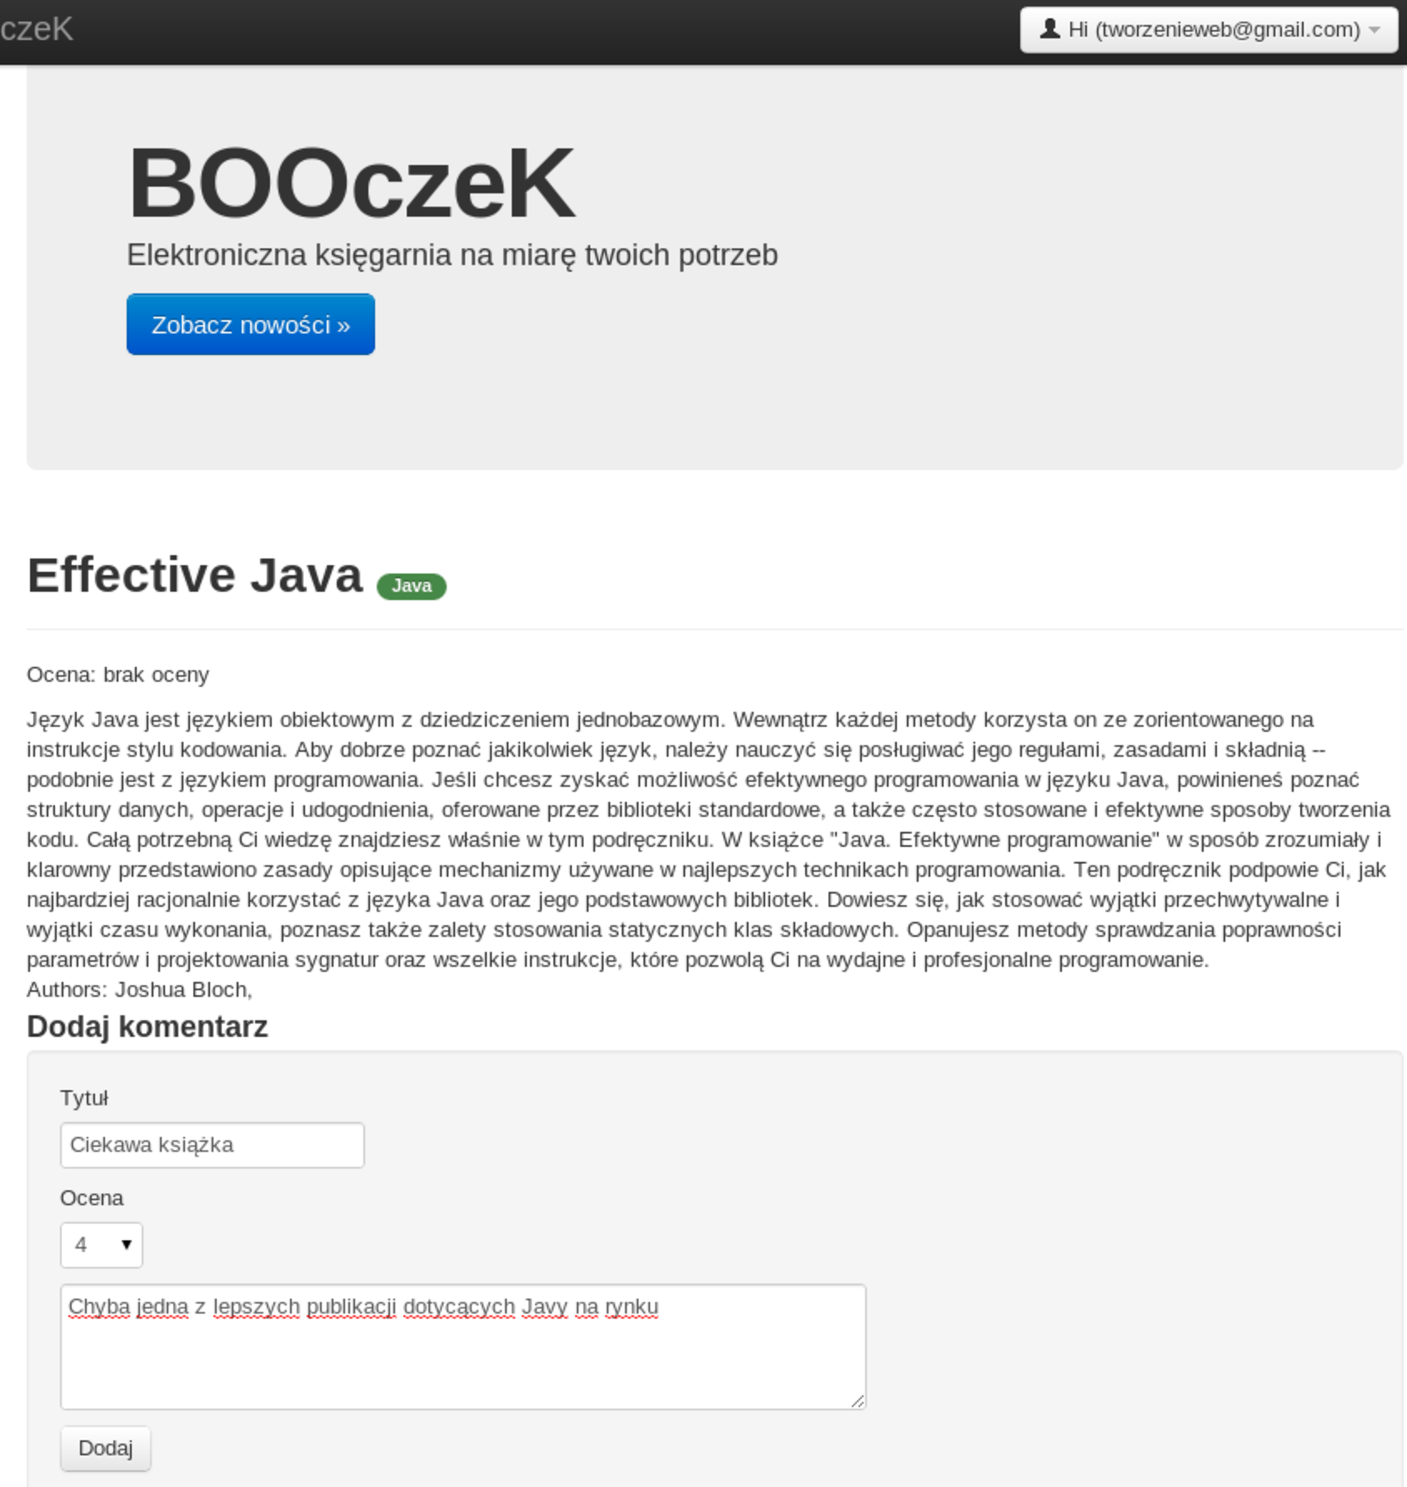
\includegraphics[scale=0.6]{frontend.pdf}
\label{fig:frontend}
\end{figure}

\section{Przetwarzanie danych pochodz�cych z \textit{webserwis�w}}

W celu rozszerzenia mo�liwo�ci j�zyka \textit{JavaScript} zastosowano framework \textit{jQuery}. Pomaga on w zapewnieniu kompatybilno�ci tworzonego kodu dla r�nych przegl�darek. Oczywi�cie w��czaj�c przegl�dark� IE6. Framework \textit{jQuery} jest szczeg�lnie przydatny ze wzgl�du na zaawansowane funkcjonalno�ci do obs�ugi zapyta� asynchronicznych AJAX. Jest to szczeg�lnie wa�ne, poniewa� razem z ��daniem i jego specyfikacj� konieczne jest, by wys�a� r�wnie� zahaszowane dane autoryzacyjne. Ca�o�� opiera si� na pierwszym zalogowaniu, podczas kt�rego do sesji u�ytkownika trafia kod autoryzacyjny u�yty do pomy�lnego zalogowania. W ten spos�b us�ugi wiedz�, �e dost�p do nich zosta� zweryfikowany. Jego brak poskutkowa�by b��dem autoryzacji - kod 401. W przysz�o�ci mo�na t� funkcjonalno�� rozszerzy� o autoryzacj� wykorzystuj�c standard \textit{OAuth 2.0}, zaimplementowany mi�dzy innymi w Twitterze lub w \textit{Facebook Graph API}.\\

Listing \ref{listing:js} przedstawia implementacj� logiki realizuj�cej wysy�anie komentarzy do webserwisu, odpowiedzialnego za dodawanie komentarzy. Do poprawnego dzia�ania konieczna jest znajomo�� nag��wka autoryzacyjnego, wi�c musi on by� przekazany do obiektu \textit{XMLHTTPRequest} jeszcze przed wys�aniem zapytania. Dodatkow� funkcjonalno�ci� jest wy�wietlanie uaktualnionych komentarzy zaraz po zapisaniu danych. Odpowiedzialna jest za to funkcja \texttt{reloadComments()}, kt�ra dodatkowo wykorzystuje now� mo�liwo�� j�zyka \textit{JavaScript}, mo�liw� dzi�ki odpowiednim wtyczkom. Polega ona na tworzeniu szablon�w, kt�re s� p�niej ��czone z danymi, tak jak to odbywa si� na przyk�ad w innych technologiach po stronie serwera. Mowa tu o \textit{Jquery Templates}, kt�re mog� w przysz�o�ci trafi� do standardu j�zyka \textit{JavaScript}.


\begin{lstlisting}[language=html, caption=Kod odpowiedzialny za realizacj� dodawania komentarzy, label=listing:js]
<script id="commentTemplate" type="text/x-jquery-tmpl"> 
    <div class="row-fluid">
          <h4>${title} {{html $item.getStars()}}</h4>
           <p>${content}</p>
          <p>${date}${user.first_name} ${user.last_name} (${user.username})</p>
    </div>
</script>

<script>
    var url = "<?php echo sfConfig::get('app_gae') . 'comments/' . $book['id'] . '/'; ?>";
    
    var reloadComments = function() {
        $("#comments").html('');
        $.getJSON(url, function(data) {
           
           /* Render the template with the data */
           $( "#commentTemplate" ).tmpl( data, { 
    getStars: function( ) {
        var str = '';
        for(i=0; i < this.data.grade; i++) {
            str += '<i class="icon-star"></i>'
        }
        
        for(j=i; j < 5; j++) {
            str += '<i class="icon-star-empty"></i>'
        }
        
        return str;
    }
}).appendTo( "#comments" );
           
       });
        
    }
    
    $(function() {
       
       reloadComments();
       
       
       $('#commentForm').submit(function (e){
           e.preventDefault();
           
           $.ajax({
               url: url,
               data: $(this).serialize(),
               xhrFields: {
                   withCredentials: true
                   
               },
               type: 'POST',
               
               beforeSend: function(xhr) {
                    xhr.setRequestHeader("Authorization", "<?php echo $sf_user->getAttribute('user_authorization', null, 'sfGuardSecurityUser') ?>");
               },
               
               success: function(data) {
                   reloadComments();
               }
           });
           
       });
       
    });
</script>
\end{lstlisting}

Jak wynika z listingu \ref{listing:js}, metoda \texttt{reloadComments()} odpowiedzialna jest za przetwarzanie danych komentarzy powi�zanych z konkretn� ksi��k� i wy�wietlenie odpowiedniej ilo�ci "gwiazdek" na podstawie oceny u�ytkownika. Jest to przyk�ad odci��enia \textit{back-endu} aplikacji, na rzecz przetwarzania po stronie klienta.

Podobny spos�b przetwarzania danych wykorzystany jest do pobierania listy kategorii dost�pnych dla ksi��ek (\ref{listing:js_cat}). Do prezentacji pojedynczego wpisu stworzono szablon. W ten spos�b w miejsca oznaczone symbolami \texttt{\${title}} i podobnymi, wstawiane s� dane z obiektu \textit{JSON}.

\begin{lstlisting}[language=html, caption=Kod odpowiedzialny za wy�wietlanie kategorii, label=listing:js_cat]
<script id="categoryTemplate" type="text/x-jquery-tmpl"> 
    <li>
        <a href="${$item.url()}">${name}
            <span class="badge badge-success">${count}</span>
        </a>
    </li>
</script>


<script>
    var urlCat = "<?php echo sfConfig::get('app_gae'); ?>categories/";
    var link = "<?php echo url_for('@category_slug?slug=' . 'slug'); ?>";
    $(function() {
        
        $.getJSON(urlCat, function(data) {
            
           /* Render the template with the movies data */
           $( "#categoryTemplate" ).tmpl( data, {
               url: function() {
                   
                   return link.replace('slug', this.data.slug);
                   
               }
           }).appendTo( "#category" );
            
        });
        
    });
    
</script>
\end{lstlisting}

\section{Optymalizacja kodu \textit{HTML} oraz zasob�w}

Optymalizacja kodu \textit{HTML} ma na celu zapewnienie szybkiego przetwarzania odpowiedzi serwera przez przegl�dark�. Jedn� z wa�niejszych optymalizacji jest usuni�cie definicji styli zawartych w znacznikach, na rzecz ujednoliconych definicji w arkuszu styli. Optymalizacja ta wprowadza uporz�dkowanie do tworzonego kodu, zmniejsza rozmiar kodu HTML oraz przyspiesza renderowanie strony przez przegl�dark�. �atwiej jest bowiem wczyta� wszystkie regu�y dekoracji znacznik�w w jednym miejscu ni� sprawdza� ka�dy znacznik z osobna \cite{book:yahoo}. 

Kolejna wa�na optymalizacja polega na redukcji ilo�ci ��da� jakie wykonuje przegl�darka. Aby to osi�gn�� nale�y wykorzysta� narz�dzia s�u��ce do kompresji kodu wynikowego \textit{JavaScript} oraz \textit{CSS}. Je�li z��czymy wszystkie arkusze styli w jeden plik, podobnie jak kod \textit{JavaScript}, ilo�� ��da� ulegnie zmniejszeniu, przyspieszaj�c jednocze�nie czas wczytywania strony. Zgodnie z \cite{book:yahoo}, dobrze jest wykorzysta� osobne serwery do sk�adowania plik�w statycznych. Poj�cie to znane jako CDN (ang. Content Delivery Network) jest szczeg�lnie rozpowszechnione w wypadku popularnych bibliotek JavaScript. Kod frameworka \textit{jQuery} umieszczony jest w�a�nie na jednym z takich serwer�w (\textit{google apis}), podobnie jak biblioteka \textit{jQuery Validate}, dokonuj�ca weryfikacji danych formularza.

Jednym z przydatnych dodatk�w do frameworka \textit{Symfony}, jest wtyczka \textit{sfCombine}, oferuj�ca du�e mo�liwo�ci w zakresie optymalizacji zasob�w. Za jej pomoc� mo�liwe jest skompresowanie i z��czenie wszystkich zasob�w \textit{JavaScript} w jeden plik, podobnie jak arkuszy \textit{CSS}. Dodatkowo wtyczka kontroluje nag��wki \textit{HTTP} wysy�ane do przegl�darki. W ten spos�b przegl�darka pobiera now� wersj� zasob�w, tylko w sytuacji, kiedy te uleg�y zmianie, w przeciwnym wypadku korzysta z lokalnej wersji. My�l�, �e nie trzeba nadmienia� jak du�o mo�na w ten spos�b osi�gn��.

\begin{figure}[htbp]
\caption{Analiza ilo�ci ��da� aplikacji ksi�garni elektronicznej bez w��czonych optymalizacji} 
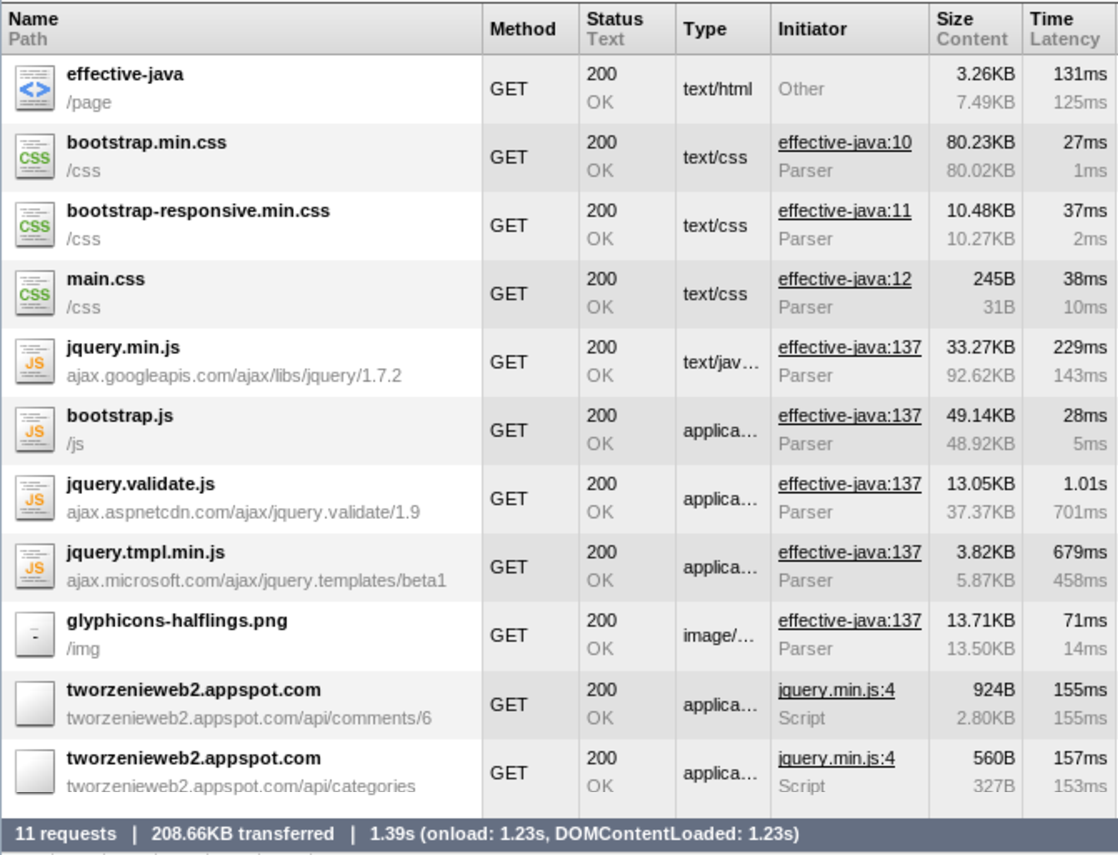
\includegraphics[scale=0.72]{minify_no.pdf}
\label{fig:minify_no}
\end{figure}

Na rysunku \ref{fig:minify_no} wida� czas oczekiwania oraz ilo�� ��da� wysy�anych do serwera w celu pobrania strony. S� to statystyki bez w��czonej wtyczki kompresuj�cej. Oczywi�cie w wypadku naszej aplikacji mamy tylko trzy arkusze styli i jeden plik \textit{Javascript} nie pochodz�cy z \textit{CDN} i przechowywany lokalnie. Korzy�ci przy w��czeni wtyczki nie powinny by�, wi�c tak znaczne, jak w przypadku aplikacji z�o�onej z kilkunastu plik�w z zasobami. Dane zawarte na rysunku \ref{fig:minify_yes}, pokazuj� jednak, �e nawet w wypadku prostej aplikacji, warto kompresowa� zawarto��. Przewidywana redukcja ��da� do 9 nie mo�e, a� jest tak imponuj�ca, jak fakt, �e ��czny czas oczekiwania uda�o si� zredukowa� o 50\%, a transfer danych zmniejszy� si� 50 razy. Jak wida�, wszystkie zasoby zwracaj� status \textit{304} okre�laj�cy, �e zasoby nie zosta�y zmodyfikowane, dzi�ki czemu serwer korzysta z lokalnej wersji.


\begin{figure}[htbp]
\caption{Analiza ��da� aplikacji ksi�garni elektronicznej z w��czon� optymalizacj�} 
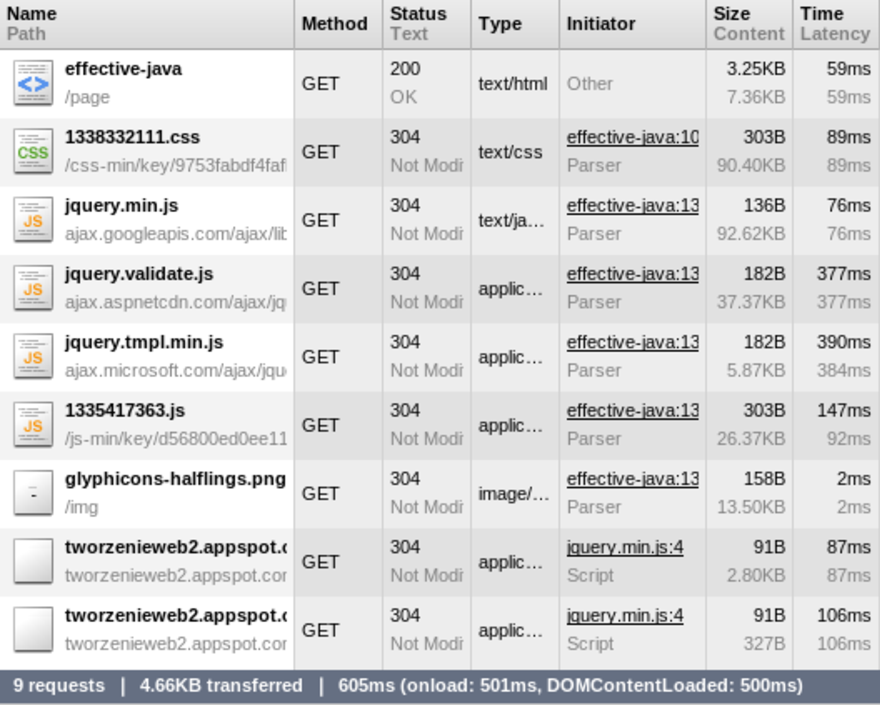
\includegraphics[scale=0.9]{minify_yes.pdf}
\label{fig:minify_yes}
\end{figure}

Optymalizacje po stronie klienta s� bardzo wa�ne, poniewa� bezpo�rednio wp�ywaj� na czas po jakim klient zobaczy stron�. Ka�dy kilobajt danych wi�cej do pobrania, odpowiednio wyd�u�a czas wczytywania strony, dlatego zastosowano kompresj� zasob�w oraz ich z��czenie. Dodatkowo dzi�ki wykorzystaniu nag��wk�w \textit{HTTP}, mo�liwe jest ograniczenie danych, kt�re pobiera przegl�darka w chwili pobierania strony.
\chapter{Optymalizacja aplikacji}
\label{cha:optymalizacja_aplikacji}

W ramach poprzednich rozdzia��w prze�ledzono szczeg�owo wszystkie istotne kwestie zwi�zane z optymalizacj� aplikacji webowych. Czas wi�c rozpocz�� praktyczn� implementacj� oprogramowania.

\section{Framework Django}
\label{section:django}

Framework \textit{Django} powsta� na bazie j�zyka Python i w nied�ugim czasie zrewolucjonizowa� proces tworzenia aplikacji internetowych w tym�e j�zyku. 

\textit{Django} posiada wszystkie cechy, kt�re charakteryzuj� narz�dzia do szybkiego tworzenia oprogramowania (\textit{ang. Rapid Application Development}). Podobnie, jak \textit{Ruby on Rails} lub \textit{Symfony}, posiada bibliotek� do mapowania obiektowo - relacyjnego. W ten spos�b definiuj�c obiektowe modele i ich metody, mo�na bez wiedzy z dziedziny baz danych wykonywa� na nich operacje. Oczywi�cie w niniejszej pracy, istotna jest kompleksowa znajomo�� zagadnie� bazodanowych, dlatego te� z jednej strony wykorzystano to narz�dzie w celu przyspieszenia procesu implementacji tworzonej aplikacji, a z drugiej strony trzeba mie� na uwadze wszystkie om�wione w poprzednich rozdzia�ach optymalizacje po stronie silnika bazodanowego.\\

Frameworki pokroju \textit{Ruby on Rails} posiadaj� atut w postaci \textit{scaffoldingu}, czyli zdolno�ci do generowania podstaw aplikacji przy u�yciu odpowiednich narz�dzi linii komend. \textit{Django} nie jest pod tym wzgl�dem wyj�tkiem, poniewa� umo�liwia generowanie zar�wno bazy aplikacji, jak r�wnie� kompletnego panelu administracyjnego, oferuj�cego zaawansowane funkcje, przydatne na przyk�ad do redagowania strony przez u�ytkownika ko�cowego bez znajomo�ci technologii.

W przypadku projektowanej ksi�garni, za pomoc� generator�w \textit{Django} mo�na w prosty spos�b zarz�dza� aplikacj� w oparciu o wcze�niej zdefiniowane modele. Oczywi�cie om�wione w poprzednim rozdziale rozszerzenie \textit{Django-Norel} umo�liwi� rozszerzenie zakresu dost�pnych baz danych o bazy nierelacyjne. 

\textit{Django-Norel} zapewnia r�wnie� narz�dzia, umo�liwiaj�ce �atwe wdro�enie tworzonego oprogramowania na platform� \textit{Google Application Engine}. Aby jednak mo�liwe by�o umieszczenie projektu na tej platformie nale�y zarejestrowa� darmowe konto. Po zweryfikowaniu jego poprawno�ci mo�liwe jest utworzenie do \textbf{10} darmowych aplikacji, ka�dej z w�asn� baz� \textit{Google Datastore} i zbiorem powi�zanych us�ug.

\section{Wystawienie us�ug jako webserwis�w}

Jednym z powod�w wyboru frameworka \textit{Django} jest �atwa mo�liwo�� tworzenia \textit{REST}owych us�ug w oparciu o istniej�ce modele. Zapewnia to wtyczka \textit{Django-Piston}, kt�ra dokonuje \textit{serializacji} do kilku popularnych format�w, w tym do notacji \textit{JSON}. Listing \ref{listing:webservice_handler} przedstawia implementacj� jednej z  us�ug (Komentarzy). Jak wida� implementacja takiej us�ugi jest dosy� prosta z wykorzystaniem wspomnianej wcze�niej wtyczki. Wystarczy stworzy� now� klas�, kt�ra dziedziczy po bazowej \texttt{BaseHandler}. Nast�pnie okre�lono dozwolone metody HTTP, odpowiedzialne za pobieranie danych, ich tworzenie, aktualizacj�, a ko�cz�c na usuwaniu. 

Piston oferuje mo�liwo�� zabezpieczania dost�pu do konkretnych zasob�w. W ten spos�b tylko osoba znaj�ca has�o mo�e doda� komentarz lub ocen�. Z drugiej strony mo�liwe jest stworzenie osobnej wersji us�ugi udost�pniaj�cej tylko okre�lone operacje. Jak wida� na listingu \ref{listing:webservice_handler}, odpowiedzialna jest za to klasa \texttt{AnonymousCommentHandler}. Wymieniona us�uga pozwala na dodanie komentarza lub ich podgl�d. Ostatnia czynno�� konieczna do wystawienia us�ugi, to jej zmapowanie na okre�lony adres zasobu. Odpowiedzialny jest za to kod z listingu \ref{listing:webservice_url}. Po wdro�eniu aplikacji mo�liwe jest sprawdzenie dzia�ania us�ugi na przyk�ad pod adresem \texttt{http://tworzenieweb.appspot.com\\/api/categories/}. Podany adres zasobu zwraca list� wszystkich kategorii, ��cznie z ilo�ci� przypisanych ksi��ek. Listing \ref{listing:webservice_response} przedstawia zwr�cony kod w notacji \textit{JSON}.

\begin{lstlisting}[language=python, caption=Implementacja us�ugi odpowiedzialnej za komentarze, label=listing:webservice_handler]
class AnonymousCommentHandler(AnonymousBaseHandler):
    model = Comment
    fields = ('title', 'content', ('user', ('id','first_name', 'last_name', 'username')), 'date', 'grade')

    def read(self, request, book_id):
        return self.model.objects.filter(book = book_id)

class CommentHandler(BaseHandler):
    anonymous = AnonymousCommentHandler
    allowed_methods = ('GET', 'PUT', 'DELETE', 'POST')
    model = Comment
    fields = ('title', 'content', ('user', ('id','first_name', 'last_name', 'username')), 'date', 'grade')   

    def read(self, request, book_id):
        
        self.anonymous.read(request, book_id)
    
    @validate(CommentForm)
    def create(self, request, book_id):
        data = request.data
        
        book = Book.objects.filter(id = book_id).exists()
        
        if not book:
            return rc.NOT_FOUND;
        
        em = self.model(
                        title=data['title'], 
                        content=data['content'], 
                        grade = data['grade'], 
                        book_id = book_id, 
                        user_id = request.user.id
                        )
        em.save()
        
            
        return rc.CREATED


\end{lstlisting}

\begin{lstlisting}[language=python,label=listing:webservice_url, caption=Wystawienie us�ugi komentarzy do publicznego dost�pu]
comment_handler = Resource(CommentHandler, authentication = auth)

urlpatterns = patterns('',
   url(r'^comments/(?P<book_id>\d+)/', comment_handler, { 'emitter_format': 'json' }),
)
\end{lstlisting}

\begin{lstlisting}[language=python,label=listing:webservice_response, caption=Rezultat zwr�cony przez us�ug� kategorii]
[
    {
        "count": 0, 
        "id": 3003, 
        "name": "Bazy Danych", 
        "slug": "bazy-danych"
    }, 
    {
        "count": 2, 
        "id": 4005, 
        "name": "Java", 
        "slug": "java"
    }, 
    {
        "count": 1, 
        "id": 13004, 
        "name": "PHP", 
        "slug": "php"
    }
]
\end{lstlisting}

\section{Uruchomienie panelu administracyjnego aplikacji}

Zgodnie z om�wionymi w podrozdziale \ref{section:django} mo�liwo�ciami frameworka \textit{Django}, po utworzeniu odpowiednich modeli, mo�liwe jest dodanie opcji administracyjnych. Rysunek \ref{fig:django_backend} pokazuje wygl�d zaplecza administracyjnego. Natomiast rysunek \ref{fig:django_backend2} pokazuje przyk�adowy formularz dodawania ksi��ki. Ciekawym udogodnieniem jest wykorzystanie biblioteki \textit{SelectMultiple} napisanej dla frameworka \textit{jQuery}, w celu wygodniejszej pracy z polami list wielokrotnego wyboru. W ten spos�b po lewej stronie umieszczone s� kategorie, autorzy niewybrani, natomiast po prawej autorzy aktualnie zaznaczeni.

\begin{figure}[htbp]
\caption{Wygl�d zaplecza administracyjnego stworzonej aplikacji}
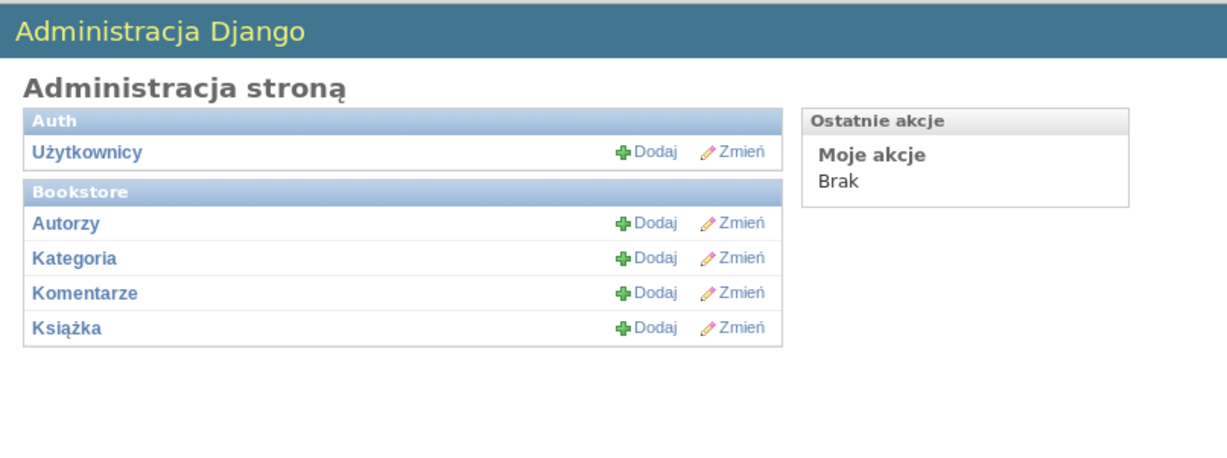
\includegraphics[scale=0.6]{django_backend.pdf}
\label{fig:django_backend}
\end{figure}

\begin{figure}[htbp]
\caption{Wygl�d zaplecza administracyjnego stworzonej ksi�garni internetowej}
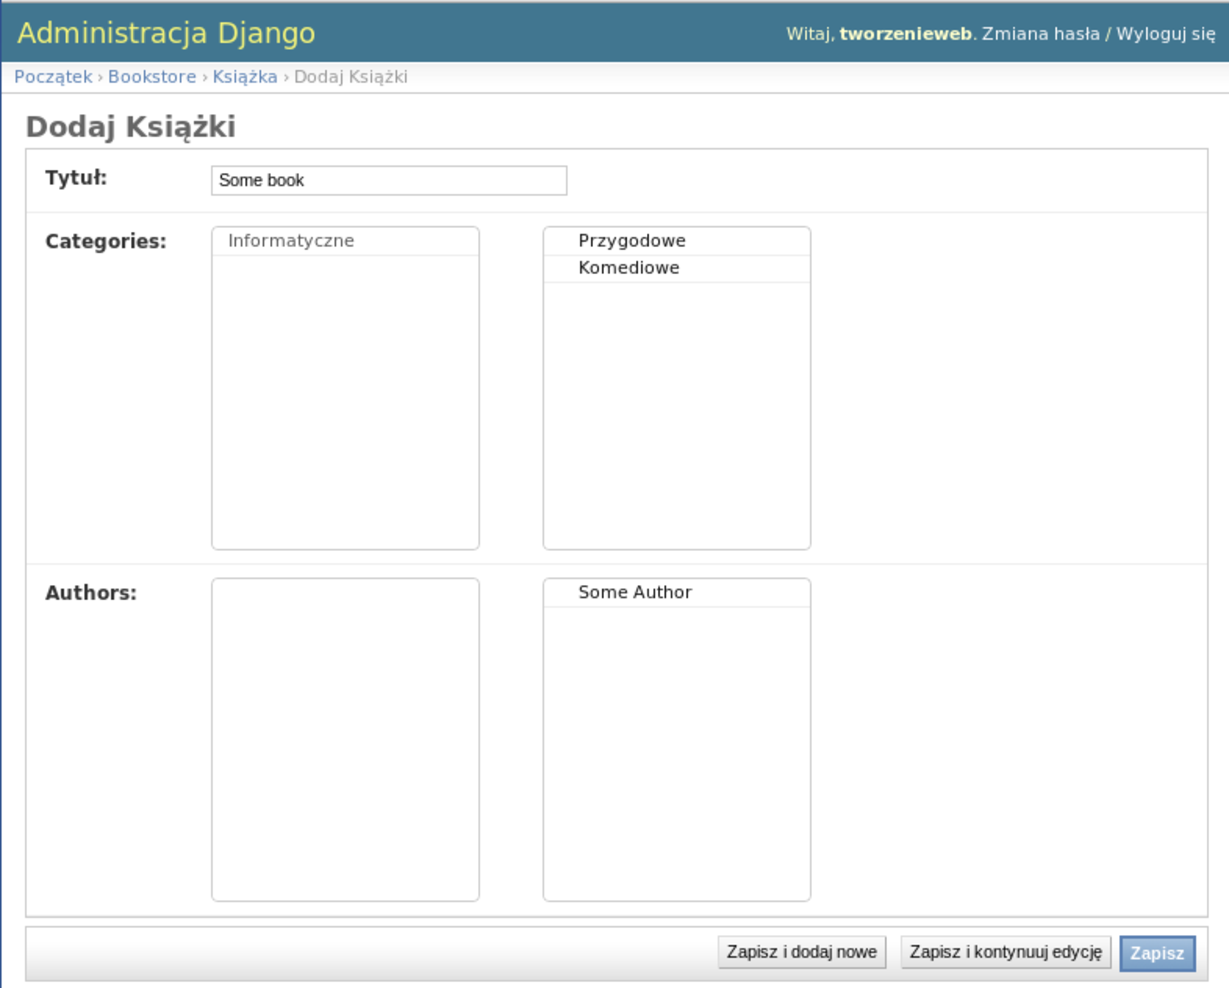
\includegraphics[scale=0.6]{django_backend2.pdf}
\label{fig:django_backend2}
\end{figure}

Jak zosta�o wykazane, framework \textit{Django} w du�ym stopniu przyspieszy� proces implementacji docelowej aplikacji na platformie \textit{Google Application Engine}. Jednym z ciekawych udogodnie� oferowanych przez GAE jest system numeracji wersji. Przyk�adowo dodano do aplikacji now� funkcjonalno��, kt�ra wymaga test�w akceptacyjnych, edytuj�c specjalny plik \texttt{app.yaml}. Parametr \texttt{version} pozwala na przyk�ad na wdro�enie aplikacji pod specjaln� subdomen� testow�. Przyk�adowo \texttt{version: staging} spowoduje, �e osobna wersja aplikacji dost�pna b�dzie pod adresem \texttt{staging.tworzenieweb.appspot.com}. Dodatkowo, w panelu administracyjnym mo�liwe jest ustawienie, kt�ra z wdro�onych aplikacji jest aplikacj� domy�ln� (Rys. \ref{fig:gae}). 

\begin{figure}[htbp]
\caption{Zarz�dzanie wersjami oprogramowania wdro�onego na platform� \textit{Google Application Engine}}
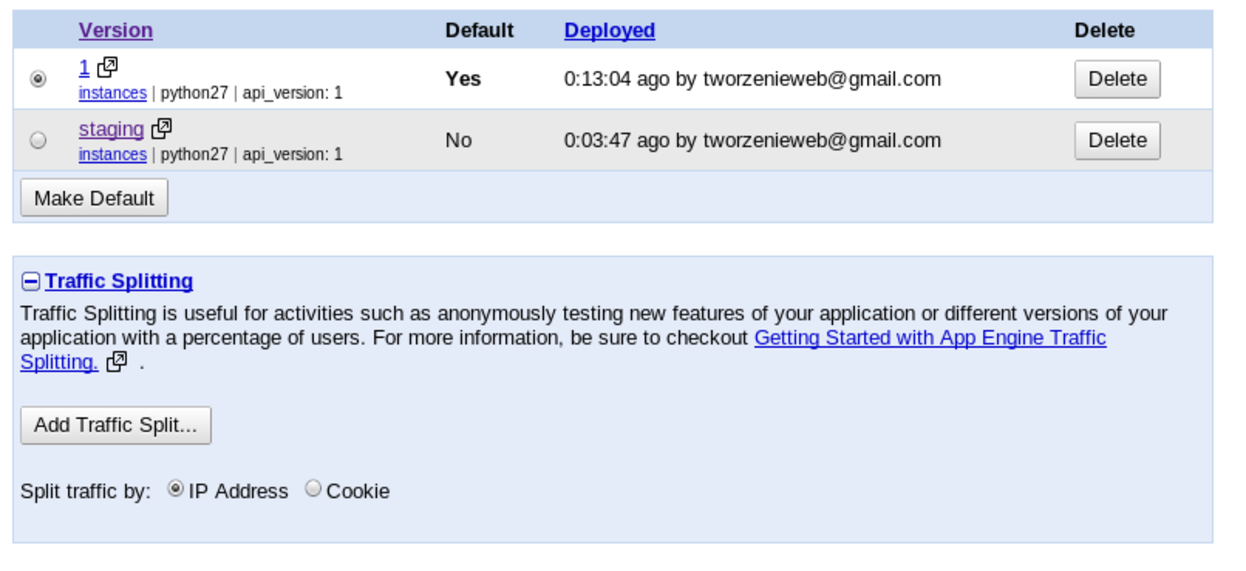
\includegraphics[scale=0.6]{gae.pdf}
\label{fig:gae}
\end{figure}


\section{Framework Symfony}

Front-end aplikacji zosta� napisany przy wykorzystaniu frameworka Symfony w wersji 1.4. Powodem wyboru tej technologii jest mo�liwo�� szybkiego tworzenia oprogramowania r�wnie� z wykorzystaniem generator�w i za�o�e� \textit{scaffoldingu}. Obecnie bardzo cz�sto daje si� zaobserwowa� ��czenie technologii w spos�b podobny do przedstawionego, czyli przyk�adowo zaplecze aplikacji i interfejs bazodanowy tworzony jest w jednej technologii na przyk�ad \textit{Django} albo \textit{Ruby on Rails}, natomiast prezentacja tre�ci jest wykonana przy u�yciu j�zyka \textit{PHP}. Dzieje si� tak, poniewa� PHP jest doskonale dostosowane do tworzenia dokument�w ko�cowych w j�zyku HTML.

Dla przyspieszenia tworzenia cz�ci przegl�dowej aplikacji, utworzono wykorzystuj�c \textit{Doctrine ORM}, schemat bazy danych to�samy z tym kt�ry znajduje si� w \textit{back-endzie}. Tak naprawd� jest on potrzebny wy��cznie do wygenerowania formularzy danych, poniewa� jak zosta�o wspomniane, operacje bazodanowe s� wykonywane wykorzystuj�c webserwisy.

Istotnym udogodnieniem w interfejsie u�ytkownika jest wykorzystanie wtyczki \textit{jQuery Validation}. Wykorzystuj�c t� bibliotek�, mo�liwe jest wykonanie sprawdzania poprawno�ci danych, wprowadzonych do poszczeg�lnych p�l.  Ca�o�� jest zintegrowana z klasami formularzy \textit{Symfony}, wi�c w momencie ustalenia przez aplikacj� rodzaju formularza, tworzony jest automatyczny plik regu� walidacji (Listing \ref{listing:reguly}), kt�ry jest nast�pnie do��czany do �r�d�a strony. Je�li kod \textit{JavaScript} jest w��czony w przegl�darce, to skrypt nie pozwoli na wys�anie formularza i b�dzie pokazywa� odpowiednie b��dy na stronie.

\begin{lstlisting}[language=java, caption=Przyk�adowy zbi�r regu� sprawdzania danych formularzy po stronie klienta, label=listing:reguly]
processForm = function(form) {
    form.submit();
}

jQuery(function($){
  
  $('#id').parents('form').validate({
    rules: {"first_name":{"maxlength":255},"last_name":{"maxlength":255},"email_address":{"required":true,"email":true},"username":{"required":true,"maxlength":128},"password":{"required":true,"maxlength":128},"password_again":{"maxlength":128}},
    messages: {"first_name":{"maxlength":function(a, elem){ return '\\\"' + $(elem).val() + '\\\" is too long (255 characters max).';}},"last_name":{"maxlength":function(a, elem){ return '\\\"' + $(elem).val() + '\\\" is too long (255 characters max).';}},"email_address":{"required":"Required.","email":"You should provide valid email address"},"username":{"required":"Required.","maxlength":function(a, elem){ return '\\\"' + $(elem).val() + '\\\" is too long (128 characters max).';}},"password":{"required":"Required.","maxlength":function(a, elem){ return '\\\"' + $(elem).val() + '\\\" is too long (128 characters max).';}},"password_again":{"maxlength":function(a, elem){ return '\\\"' + $(elem).val() + '\\\" is too long (128 characters max).';}}},
    onkeyup: false,
    wrapper: 'span class="help-inline"',
    errorElement: 'span',
    errorPlacement: function(error, element) 
    {
    
     element.parent().parent().addClass('error');
    
     if(element.parents('.radio_list').is('*') || element.parents('.checkbox_list').is('*'))
     {
       error.appendTo( element.parent().parent().parent() );
     }
     else
     {
       error.appendTo( element.parent() );
     }

   },
   submitHandler: function(form) {
     
    processForm(form);
     
   }
  
  });
  
  $('#password_again').rules('add', {"equalTo":"#password","messages":{"equalTo":"The two passwords must be the same."}});
      
});

/* for some reason the jQuery Validate plugin does not incluce a generic regex method */
jQuery.validator.addMethod(
  "regex",
  function(value, element, regexp) {
      if (regexp.constructor != RegExp)
          regexp = new RegExp(regexp);
      else if (regexp.global)
          regexp.lastIndex = 0;
      return this.optional(element) || regexp.test(value);
  },
  "Invalid."
);
\end{lstlisting}

Rysunek \ref{fig:register_validation} pokazuje rezultat dzia�ania walidacji formularza Dopiero kiedy wszystkie b��dy zostan� poprawione, skrypt pozwoli na wys�anie ��dania typu POST do docelowej us�ugi. Takie podej�cie w du�ym stopniu ogranicza ruch sieciowy w aplikacji. Oczywi�cie opr�cz walidacji danych po stronie klienta, nale�y r�wnie� bezwzgl�dnie sprawdza� dane po stronie serwera, poniewa� mo�e to prowadzi� do znacznych uchybie� w bezpiecze�stwie aplikacji.\\

Innym wa�nym udogodnieniem jest modyfikacja istniej�cej wtyczki, odpowiedzialnej za ochron� dost�pu do aplikacji. Wtyczka \textit{sfDoctrineGuardPlugin} z za�o�enia dzia�a�a z baz� danych, wi�c w punktach odpowiedzialnych za logowanie do aplikacji, pobieranie obiektu u�ytkownika lub tworzenie nowego profilu, nale�a�o zmodyfikowa� kod. W ten spos�b zamiast wykonywa� zapytania do bazy, serwer lub obiekt \textit{XMLHttpRequest} wysy�a ��danie do aplikacji na platformie GAE i przetwarza zwr�cony rezultat. W wypadku uwierzytelnienia konieczne jest zapisanie danych u�ytkownika do sesji, wi�c od tej pory aplikacja zapami�ta skojarzony obiekt u�ytkownika.

\begin{figure}[H]
\caption{Wynik dzia�ania wtyczki \textit{jQuery validation}}
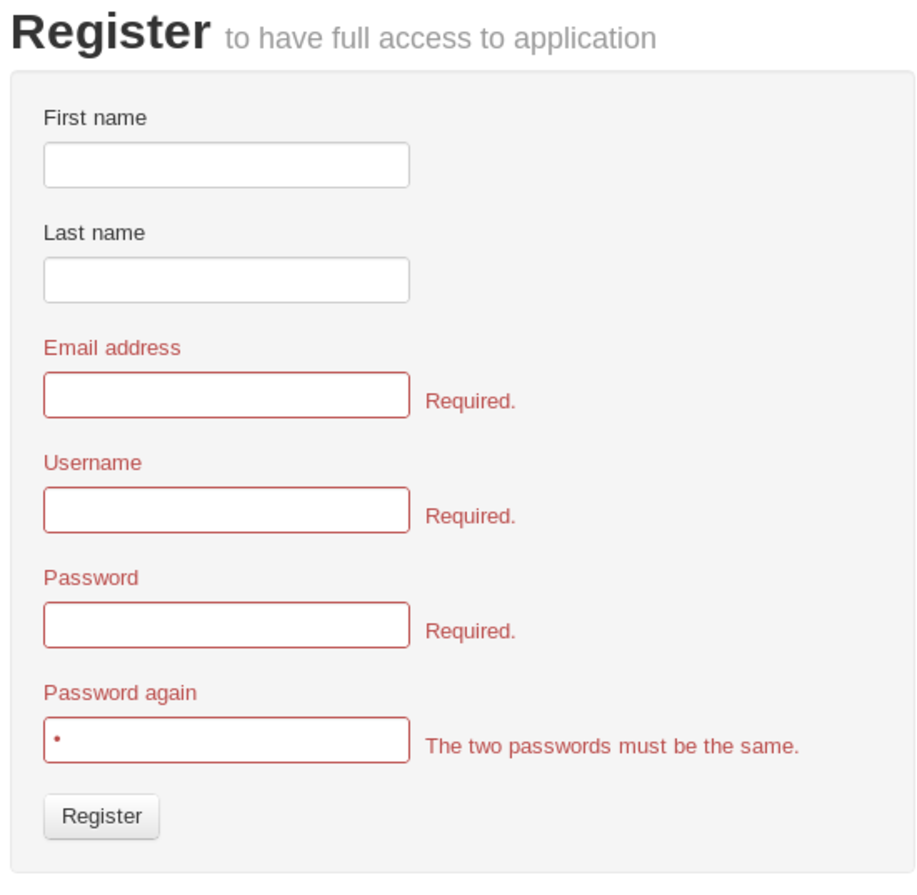
\includegraphics[scale=0.7]{register_validation.pdf}
\label{fig:register_validation}
\end{figure}


\section{Test wydajno�ci \textit{webserwis�w}}

W celu sprawdzenia faktycznej wydajno�ci us�ug, wykonano kilka test�w sprawdzaj�cych zar�wno dzia�anie operacji odczytu, jak r�wnie� zapisu.
Jak wida� na listingu \ref{listing:testgae}, test przeszed� bardzo sprawnie, osi�gaj�c liczb� prawie 60 ��da� na sekund�. Test by� przeprowadzany dla \textbf{100} u�ytkownik�w jednocze�nie. Nast�pnie zosta�a sprawdzona us�uga komentarzy (Listing \ref{listing:testkoment}). W wypadku komentarzy test wypad� troch� gorzej, ale zwi�zane jest to z wi�kszym skomplikowaniem tej us�ugi i wi�ksz� ilo�ci� danych do pobrania. Wynik \textbf{37.6} ��dania na sekund� jest bardzo wysok� warto�ci� i z pewno�ci� gwarantuje szybkie dzia�anie aplikacji.\\

Dodatkowo, w celu przyspieszenia operacji odczytu w encjach \textit{kategorii} oraz \textit{ksi��ek} przechowywane s� informacje o �redniej ocen pochodz�ce z komentarzy, jak r�wnie� ilo�� ksi��ek przechowywana w danej kategorii. Oznacza to pewn� nadmiarowo��, ale jest ona konieczna w tego typu rozwi�zaniach i powszechnie stosowana.\\

Jak wida� na listingu \ref{listing:testfrontend}, odci��enie \textit{front-endu} testowane na lokalnym komputerze r�wnie skutecznie radzi sobie z obs�u�eniem skokowym 100 u�ytkownik�w. W przysz�o�ci mo�na przenie�� kod \textit{front-endu} r�wnie� na jedno z rozwi�za� opartych na chmurze dla j�zyka \textit{PHP}. Oferuje to na przyk�ad hosting \textit{pagoda box} (\texttt{https://pagodabox.com/}). Na lokalnym �rodowisku testowym wykorzystano serwer \textit{Ngnix}, kt�ry cechuje si� du�o mniejszym narzutem pami�ci ni� np. serwer \textit{Http Apache}.

\begin{lstlisting}[label=listing:testgae, caption=Test wydajno�ci us�ugi pobierania kategorii w ramach stworzonej aplikacji]
Server Software:        Google
Server Hostname:        tworzenieweb2.appspot.com

Document Path:          /api/categories
Document Length:        0 bytes

Concurrency Level:      100
Time taken for tests:   1.721 seconds
Complete requests:      100
Failed requests:        0
Write errors:           0
Requests per second:    58.11 [#/sec] (mean)
Time per request:       1720.744 [ms] (mean)
Time per request:       17.207 [ms] (mean, across all concurrent requests)
Transfer rate:          12.20 [Kbytes/sec] received

Connection Times (ms)
              min  mean[+/-sd] median   max
Connect:       86  174  48.5    175     256
Processing:   294  765 297.3    796    1466
Waiting:      293  764 297.2    794    1465
Total:        379  939 328.0    931    1718

\end{lstlisting}


\begin{lstlisting}[label=listing:testkoment, caption=Test wydajno�ci us�ugi komentarzy]
Server Software:        Google
Server Hostname:        tworzenieweb2.appspot.com

Document Path:          /api/comments/6/


Concurrency Level:      100
Time taken for tests:   7.879 seconds
Complete requests:      100
Failed requests:        0
Write errors:           0
Total transferred:      243500 bytes
HTML transferred:       210200 bytes
Requests per second:    37.59 [#/sec] (mean)
Time per request:       27879.412 [ms] (mean)
Time per request:       278.794 [ms] (mean, across all concurrent requests)
Transfer rate:          8.53 [Kbytes/sec] received

Connection Times (ms)
              min  mean[+/-sd] median   max
Connect:       64 121 60     68   270
Processing:   270  761 332.0    723    1647
Waiting:      268  760 332.0    722    1646
Total:        339 1014 3563.3    847   16173


\end{lstlisting}

\begin{lstlisting}[caption=Test \textit{front-endu} aplikacji na lokalnym komputerze, label=listing:testfrontend]
Server Software:        nginx/1.1.19
Server Hostname:        thesis.web.dev
Server Port:            80

Document Path:          /
Document Length:        6621 bytes

Concurrency Level:      100
Time taken for tests:   2.747 seconds
Complete requests:      100
Failed requests:        0
Write errors:           0
Total transferred:      694500 bytes
HTML transferred:       662100 bytes
Requests per second:    36.40 [#/sec] (mean)
Time per request:       2747.185 [ms] (mean)
Time per request:       27.472 [ms] (mean, across all concurrent requests)
Transfer rate:          246.88 [Kbytes/sec] received

Connection Times (ms)
              min  mean[+/-sd] median   max
Connect:        2    3   0.8      3       5
Processing:    77 1496 801.5   1509    2742
Waiting:       77 1496 801.5   1509    2742
Total:         82 1499 801.7   1512    2746


\end{lstlisting}

Potencja� aplikacji wynikaj�cy z uzyskanych wynik�w, pokazuje, �e rozproszenie us�ug ma g��boki sens i przynosi wymierne rezultaty. Celem pracy nie by�o pokazanie wy��cznie korzy�ci zwi�zanych z wydajno�ci� aplikacji. Dzi�ki dekompozycji aplikacji na warstw� us�ugow� (webserwisy) i warstw� prezentacyjn� zyskujemy du�� elastyczno��. W ka�dej chwili mo�na podmieni� platform� \textit{GAE} na zupe�nie inne rozwi�zanie, maj�c na uwadze zachowanie struktury obiekt�w zwracanych przez webserwisy. Nie wp�ynie to w �adnym stopniu na dzia�anie cz�ci prezentacyjnej. Wa�ne jest jednak by obiekty \textit{JSON} pasowa�y do wcze�niej ustalonej struktury.

Opr�cz optymalizacji \textit{back-endu} aplikacji, nie bez znaczenia jest r�wnie� praca wykonana po stronie \textit{front-endu}. Implementacja pocz�tkowej walidacji danych z wykorzystaniem \textit{JavaScriptu}, pozwoli na szybsz� detekcje b��d�w w formularzach, co z pewno�ci� doceni� u�ytkownicy. Z drugiej strony moment wys�ania ��dania do serwera zostaje op�niony do momentu kiedy jest ju� du�a pewno�� prawid�owo�ci danych.

Asynchroniczne pobieranie komentarzy to kolejny krok poprawiaj�cy jako�� stworzonej aplikacji. W podej�ciu synchronicznym, na pocz�tku pobrano by z bazy dane o ksi��ce, nast�pnie dane o komentarzach powi�zanych ze stron�. Dzi�ki technologii \textit{AJAX}, te dwa zadania mog� by� wykonywane jednocze�nie. Serwer WWW generuje tylko absolutn� podstaw� strony, pozosta�e komponenty s� do��czane w mi�dzyczasie. Przek�adaj�c om�wione zagadnienie na bardziej �yciowe por�wnanie - o ile szybciej mo�liwe jest wybudowanie domu, je�li jednocze�nie kopane s� fundamenty, stawiane mury domu i k�adziony dach.
\chapter*{Podsumowanie}

Podsumowanie

\addcontentsline{toc}{chapter}{Spis rysunk�w}
\listoffigures
\addcontentsline{toc}{chapter}{Spis listing�w}
\lstlistoflistings

\addcontentsline{toc}{chapter}{Bibliografia}
\bibliographystyle{plabbrv}
\bibliography{bibliography.bib}

\addcontentsline{toc}{chapter}{Abstract}

\begin{abstract}
Nowadays Internet has been used as a wide range marketing and business tool. Most people use Internet in various fields of life. For this reason, sites and web applications becomes crowded and overloaded. Some times they can even stop working which will result in loss of money. That is why creating of high performance and stable applications is so important today. Also giving possibility to access page by huge amount of users can be cost-effective, when we put some commercials.\\

Last but not least web application architecture needs to be considered. It is very common that companies use expensive hosting solutions, that don't actually fit their needs. On the another hand,  when periodically massive traffic comes, their servers cannot handle this. That is why cloud service providers are considered to be a good alternative in this situations because companies pay only for resources actually used and nothing more.

This master thesis will cover the topic of efficiency optimization of web applications. It will be splitted into three main areas of optimizations. Firstly the optimization of application architecture will be considered and then other issues like frontend optimization as well as database and webserver tuning will be discussed. Also, this thesis needs to provide some useful tools and techniques that need to be used for mesuring of actual application performance and availability. Without this knowledge we cannot even start the main part of optimization because we do not find the typical bottlenecks.
\end{abstract}

\chapter*{P�yta CD}
\label{cha:plyta}
\thispagestyle{empty}
\pagestyle{empty}

Wraz z tre�ci� pracy dyplomowej do��czono r�wnie� p�yt� CD z kompletnym kodem �r�d�owym aplikacji. Dodatkowo kod mo�na pobra� z poni�szego repozytorium GIT: \texttt{https://github.com/tworzenieweb/Master-Thesis.git}


\end{document}
